\documentclass{beamer}
\usepackage{beamerthemeshadow}
\setbeamertemplate{headline}{}
\usefonttheme[onlymath]{serif}
\usepackage{tikz}
\usepackage{graphicx} 
\usepackage{tabularx}
\usepackage{adjustbox}

% \usepackage{media9}
% \usepackage{graphicx}
\usepackage{multimedia}
\usepackage[makeroom]{cancel}
\usetikzlibrary{arrows}
\usetikzlibrary{positioning}
% set arrows as stealth fighter jets
\tikzset{>=stealth}
% \usepackage{multicol}
% \setlength{\columnsep}{1cm}
% \usepackage[thinlines]{easytable}
% \begin{document}



\newtheorem{mydef}{Definition}
\newtheorem{mythm}{Theorem}
\newtheorem{myprop}{Proposition}
\newtheorem{lem}[mythm]{Lemma}
\newtheorem{rem}[mythm]{Remark}
\newtheorem{ex}{Example}
\newtheorem{cor}[mythm]{Corollary}

\def\Xint#1{\mathchoice
{\XXint\displaystyle\textstyle{#1}}%
{\XXint\textstyle\scriptstyle{#1}}%
{\XXint\scriptstyle\scriptscriptstyle{#1}}%
{\XXint\scriptscriptstyle%
\scriptscriptstyle{#1}}%
\!\int}
\def\XXint#1#2#3{{\setbox0=\hbox{$#1{#2#3}{%
\int}$ }
\vcenter{\hbox{$#2#3$ }}\kern-.6\wd0}}
\def\ddashint{\Xint=}
\def\dashint{\Xint-}



\DeclareMathOperator{\spn}{span}
\DeclareMathOperator{\rnk}{rank}
\DeclareMathOperator{\id}{id}
\DeclareMathOperator{\dom}{dom}
%\DeclareMathOperator{\dim}{dim}
\DeclareMathOperator{\Hom}{Hom}
\DeclareMathOperator{\Ima}{Im}
\DeclareMathOperator{\Alt}{Alt}
\DeclareMathOperator{\sign}{sign}
\DeclareMathOperator{\Img}{Img}
\DeclareMathOperator{\Diff}{Diff}
\DeclareMathOperator{\Aut}{Aut}
\DeclareMathOperator{\End}{End}
\DeclareMathOperator{\Der}{Der}
\DeclareMathOperator{\degr}{deg}

\DeclareRobustCommand\longtwoheadrightarrow
     {\relbar\joinrel\twoheadrightarrow}

% Probability symbols
\newcommand{\Pro}[2]{{\mathbb P}\left[ #1\,;\,#2\right]}
\newcommand{\CondPro}[4]{{\mathbb P}\left[ \,#1\,;\,#2\,\big|\,#3\,;\,#4\,\right]}
\newcommand{\ome}{\langle \boldsymbol \omega\rangle}
     
     

\newcommand{\red}[1]{{\color{red} #1}}
\newcommand{\green}[1]{{\color{green} #1}}

\newcommand{\lb}{\big[\!\!\big[}
\newcommand{\rb}{\big]\!\!\big]}
\newcommand{\expo}[1]{\text{e}^{#1}}
%\newcommand{\eqref}[1]{(\ref{#1})}
\newcommand{\partially}[2]{\frac{\partial #1}{\partial #2}}
\newcommand{\doublepartially}[3]{\frac{\partial^2 #1}{\partial #2\partial #3}}
\newcommand{\parOp}[1]{\frac{\partial}{\partial #1}}
\newcommand{\del}[1]{\partial_{#1}}
\newcommand{\dblul}[1]{\underline{\underline{#1}}}
\newcommand{\trpul}[1]{\underline{\underline{\underline{#1}}}}


\newcommand{\norm}[1]{\left\lVert#1\right\rVert}
% \usepackage{tagging}
% \usetag{St}
% \newcommand{\Start}{\begin{taggedblock}{St}}
% Note: A command including \end{taggedblock} produces errors

\beamertemplatenavigationsymbolsempty

\begin{document}


% \Start
\title{Gillespie Algorithm}  
\author{Leonhard Horstmeyer}
\date{\today} 

\frame{\titlepage} 

\section{Title Page}

\begin{frame}
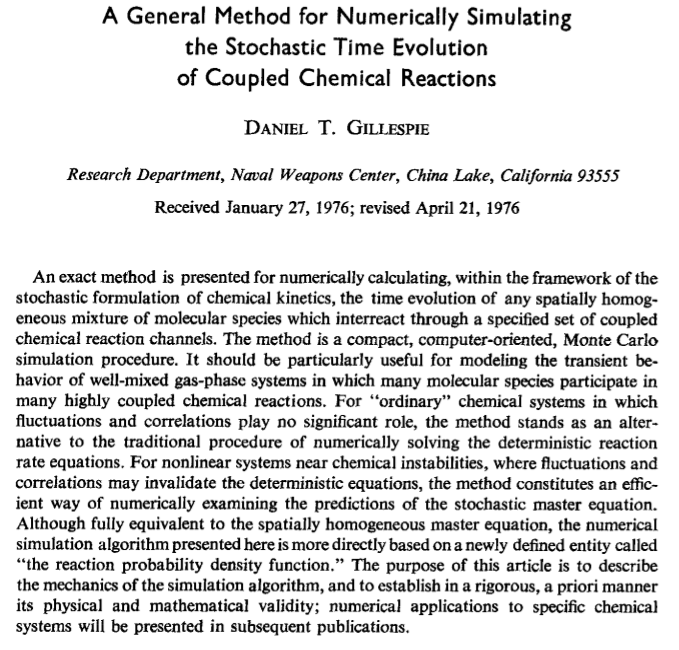
\includegraphics[width=\textwidth]{originalpapercropped.png}
\end{frame}

\begin{frame}
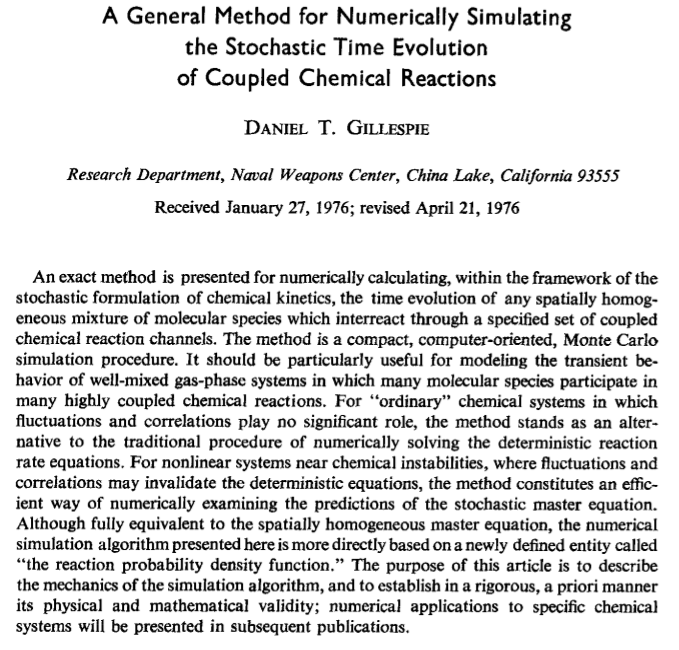
\includegraphics[width=\textwidth]{originalpapercropped.png}
\end{frame}


\section{Part I}
% 
% \begin{frame}
%  \frametitle{Gillespie's example}
% \end{frame}
% 

% \begin{frame}
%  Overview\\
%  Short note on how to find good articles on the Gillespie algorithm.
%  Gillespie for molecules als aufhaenger
%  Theory of Gillespie alg.
%  Gillespie for molecules in container
%  Gillespie for reactions
%  Gillespie for networks
%  My Gillespie implementation of the SIS w model.
% \end{frame}


\section{The Algorithm}

\begin{frame}
 \frametitle{Species}
\centering
\adjustbox{max height=\dimexpr\textheight-5.5cm\relax,
           max width=\textwidth}{
\begin{tabular}{rcccc}
\onslide<1-> \textbf{Species :} &     \begin{minipage}{.3\textwidth}
      \onslide<2->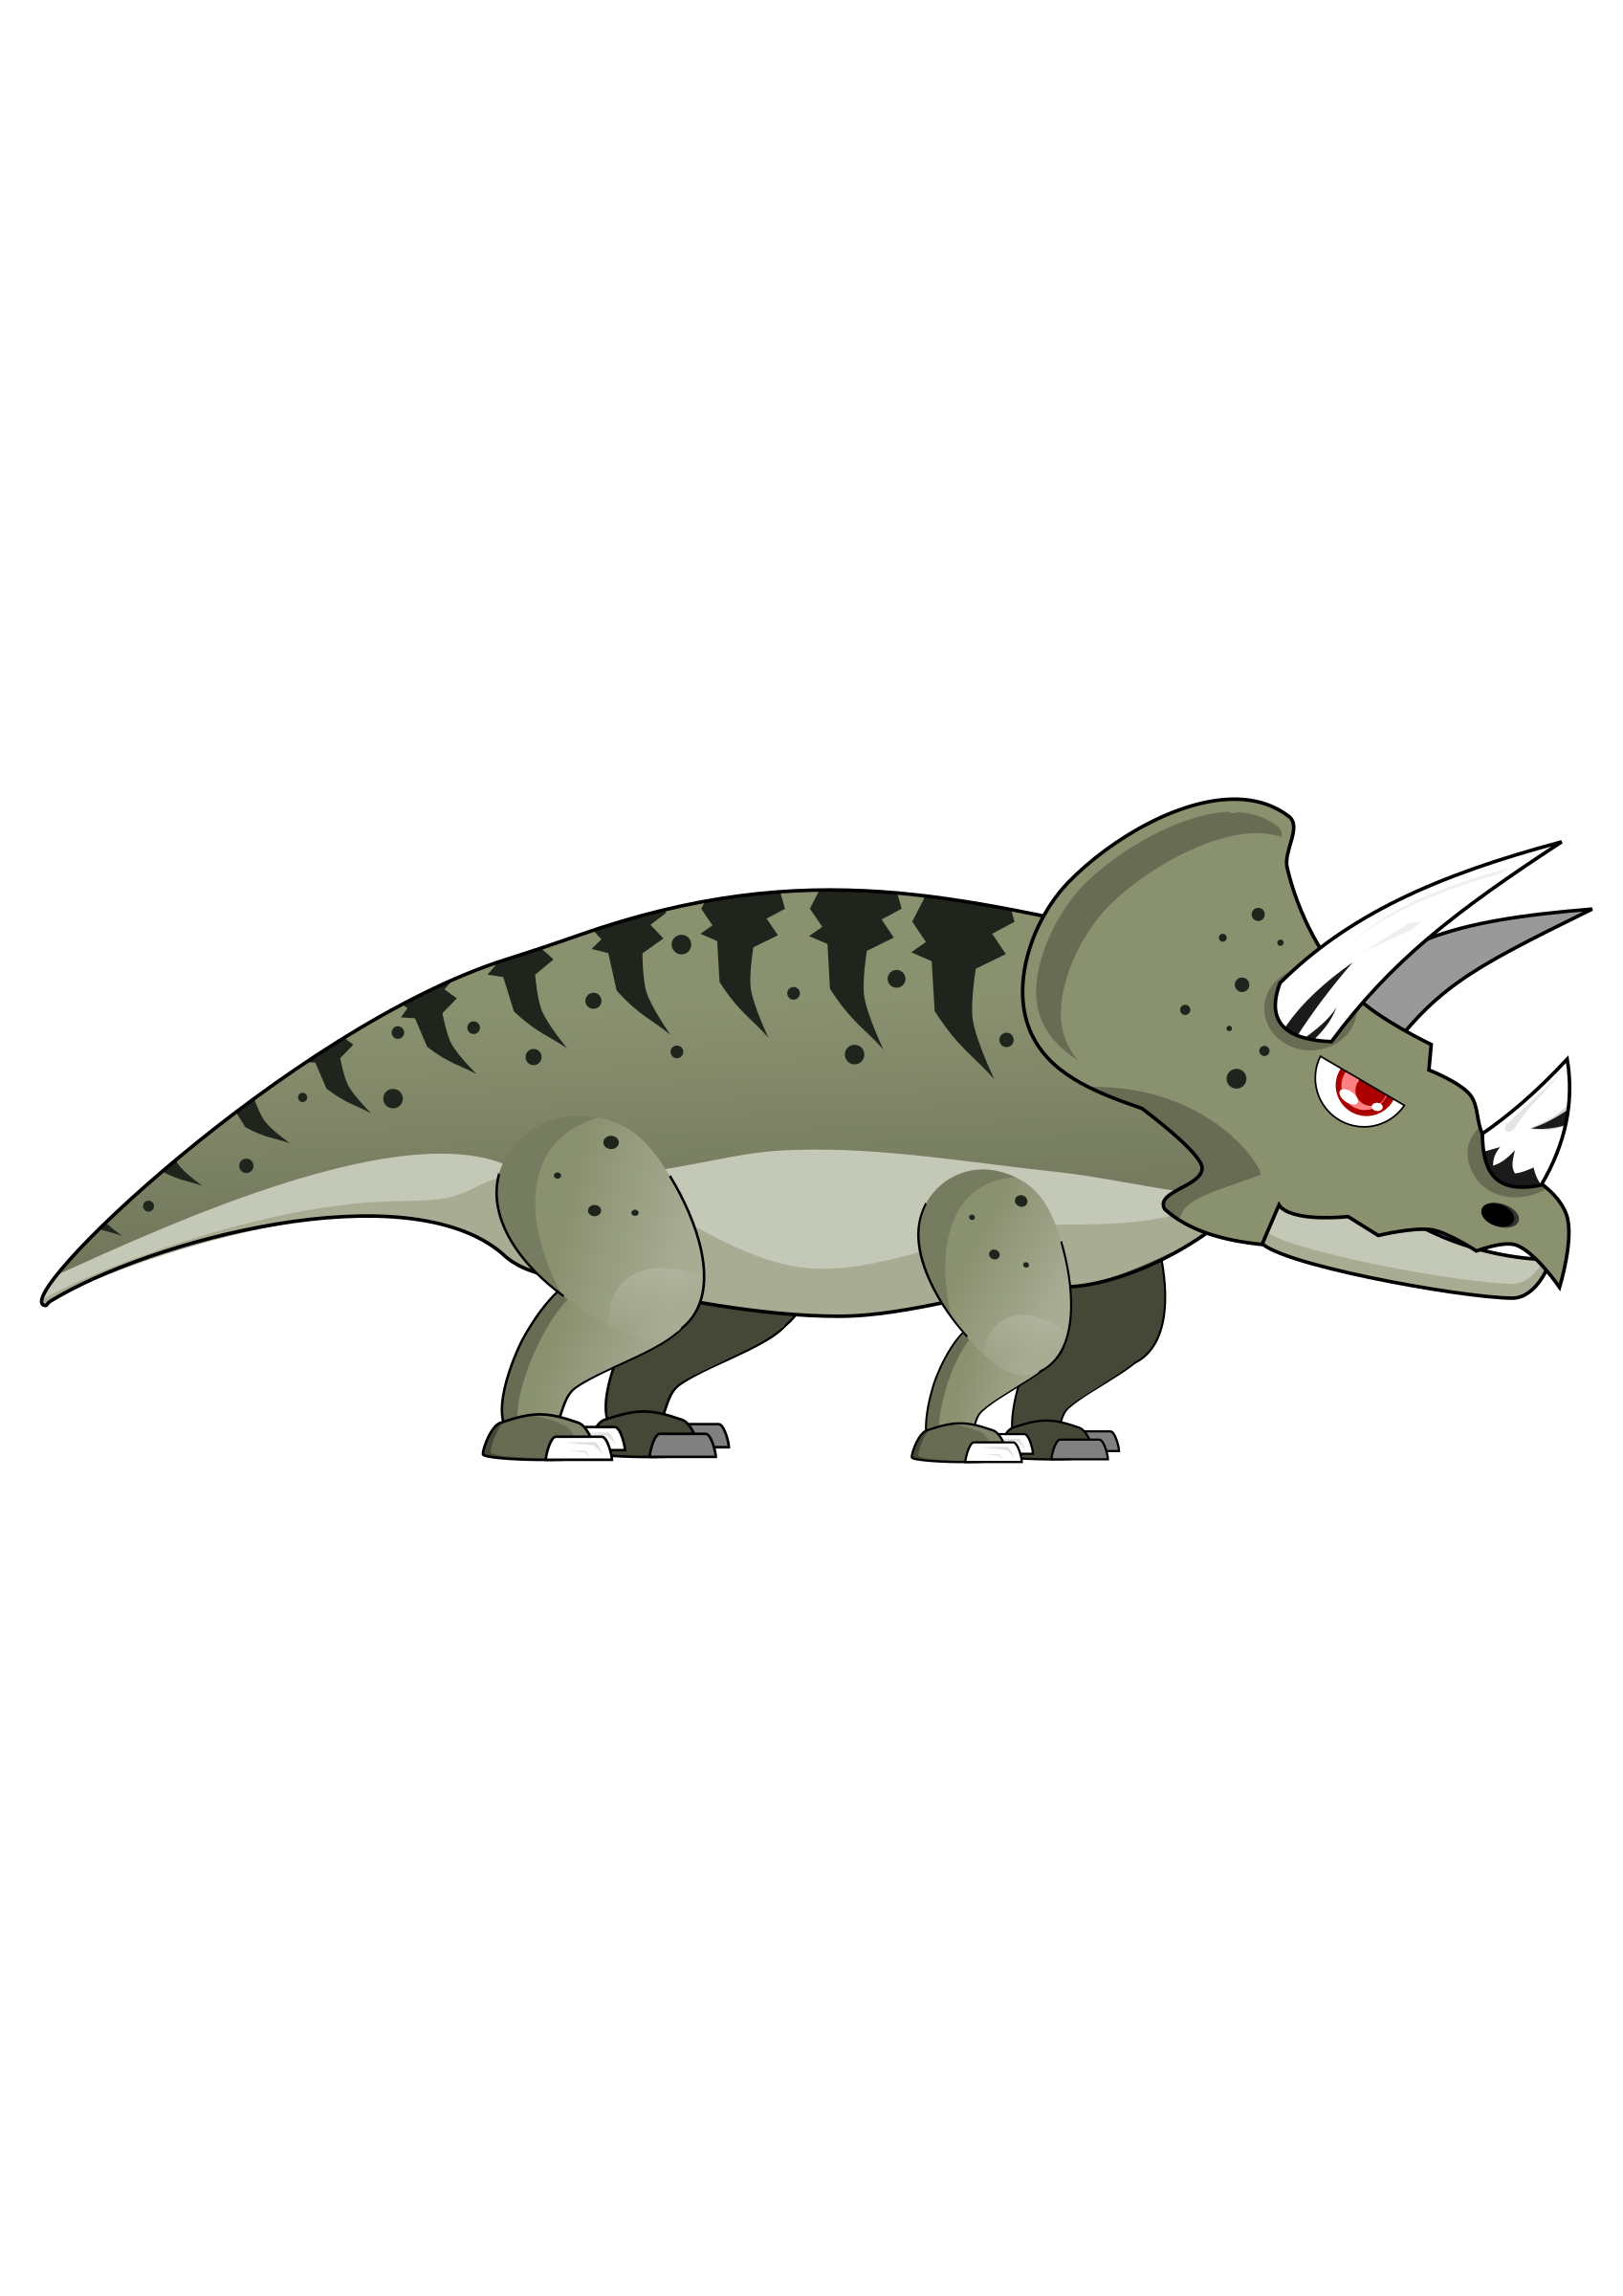
\includegraphics[width=\linewidth]{dinosaur2.png}
    \end{minipage} &  \begin{minipage}{.3\textwidth}
      \onslide<3->
\includegraphics[width=.6\linewidth]{tiger.png}
    \end{minipage} & \onslide<4-> $\dots$  & 
    \begin{minipage}{.3\textwidth}
      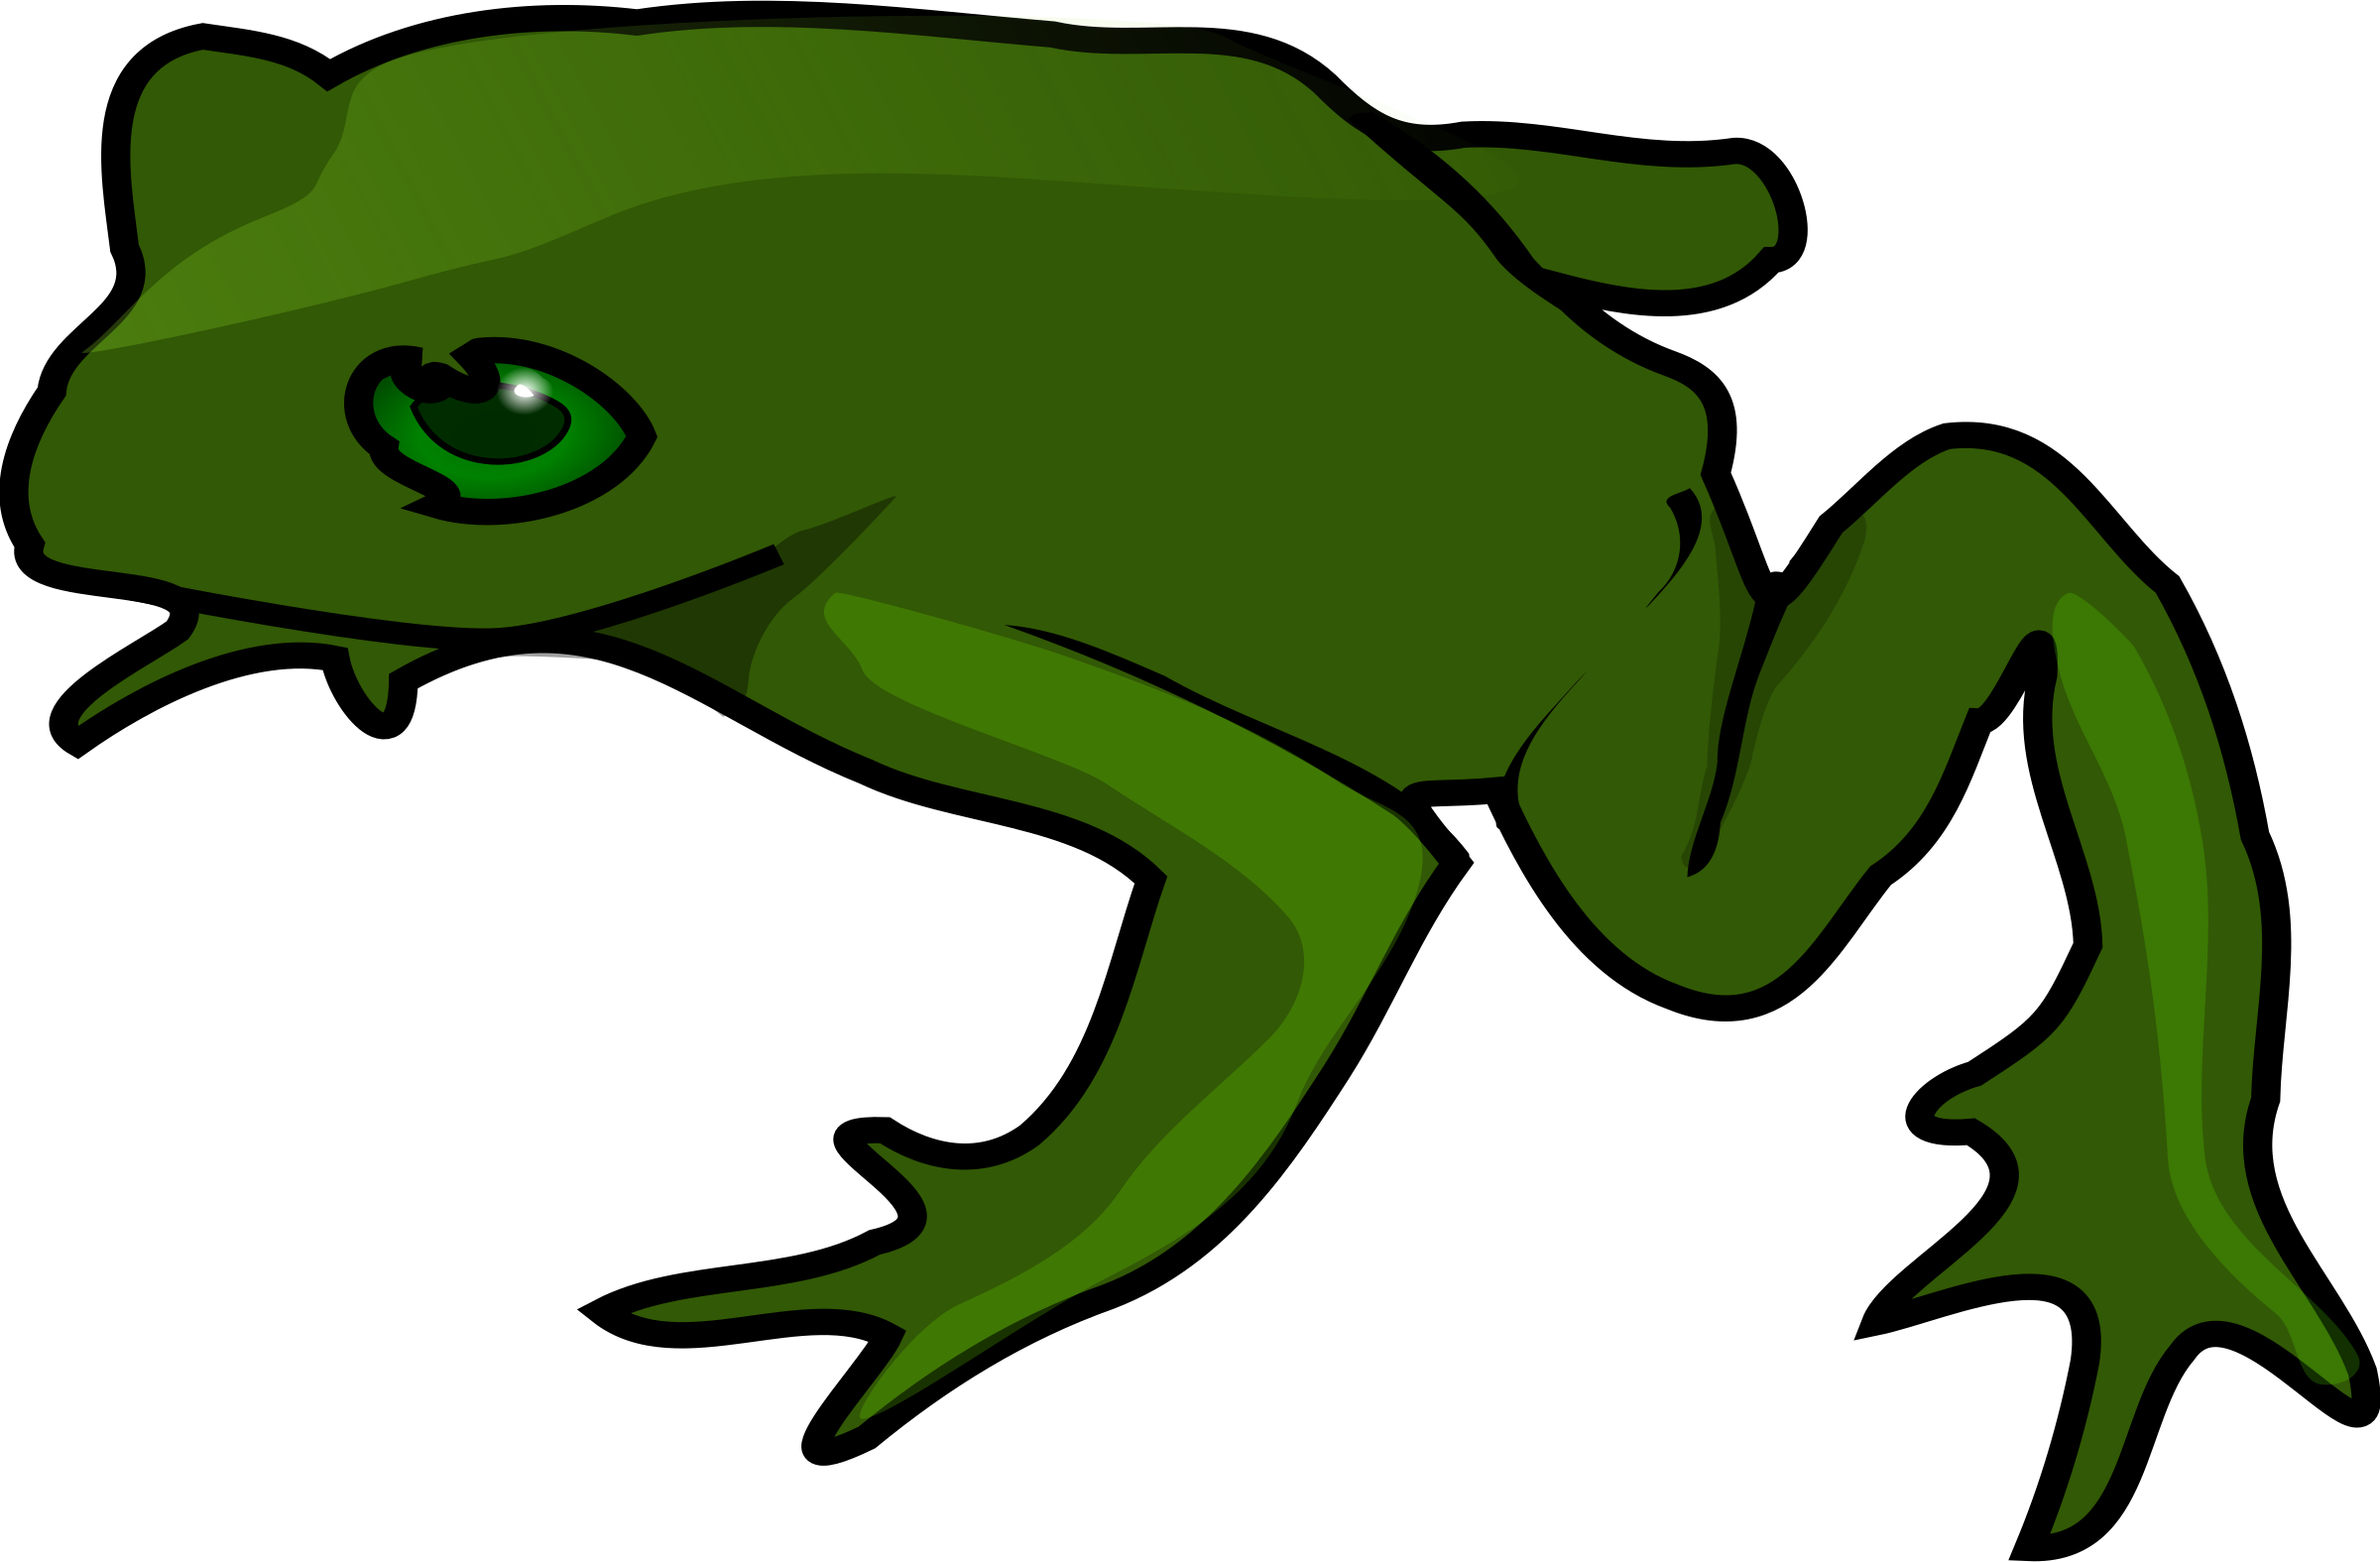
\includegraphics[width=.8\linewidth]{frog.png}
    \end{minipage}\\
 \onslide<5-> \textbf{Abundances :} & \onslide<6->$N_1$ & $N_2$ & $\dots$ & $N_S$  
\end{tabular}
}

\end{frame}

\begin{frame}
 \frametitle{Reactions}
\centering
\adjustbox{max height=\dimexpr\textheight-5.5cm\relax,
           max width=\textwidth}{
\begin{tabular}{rccccc}
   &     
    \begin{minipage}{.3\textwidth}
      \uncover<2->{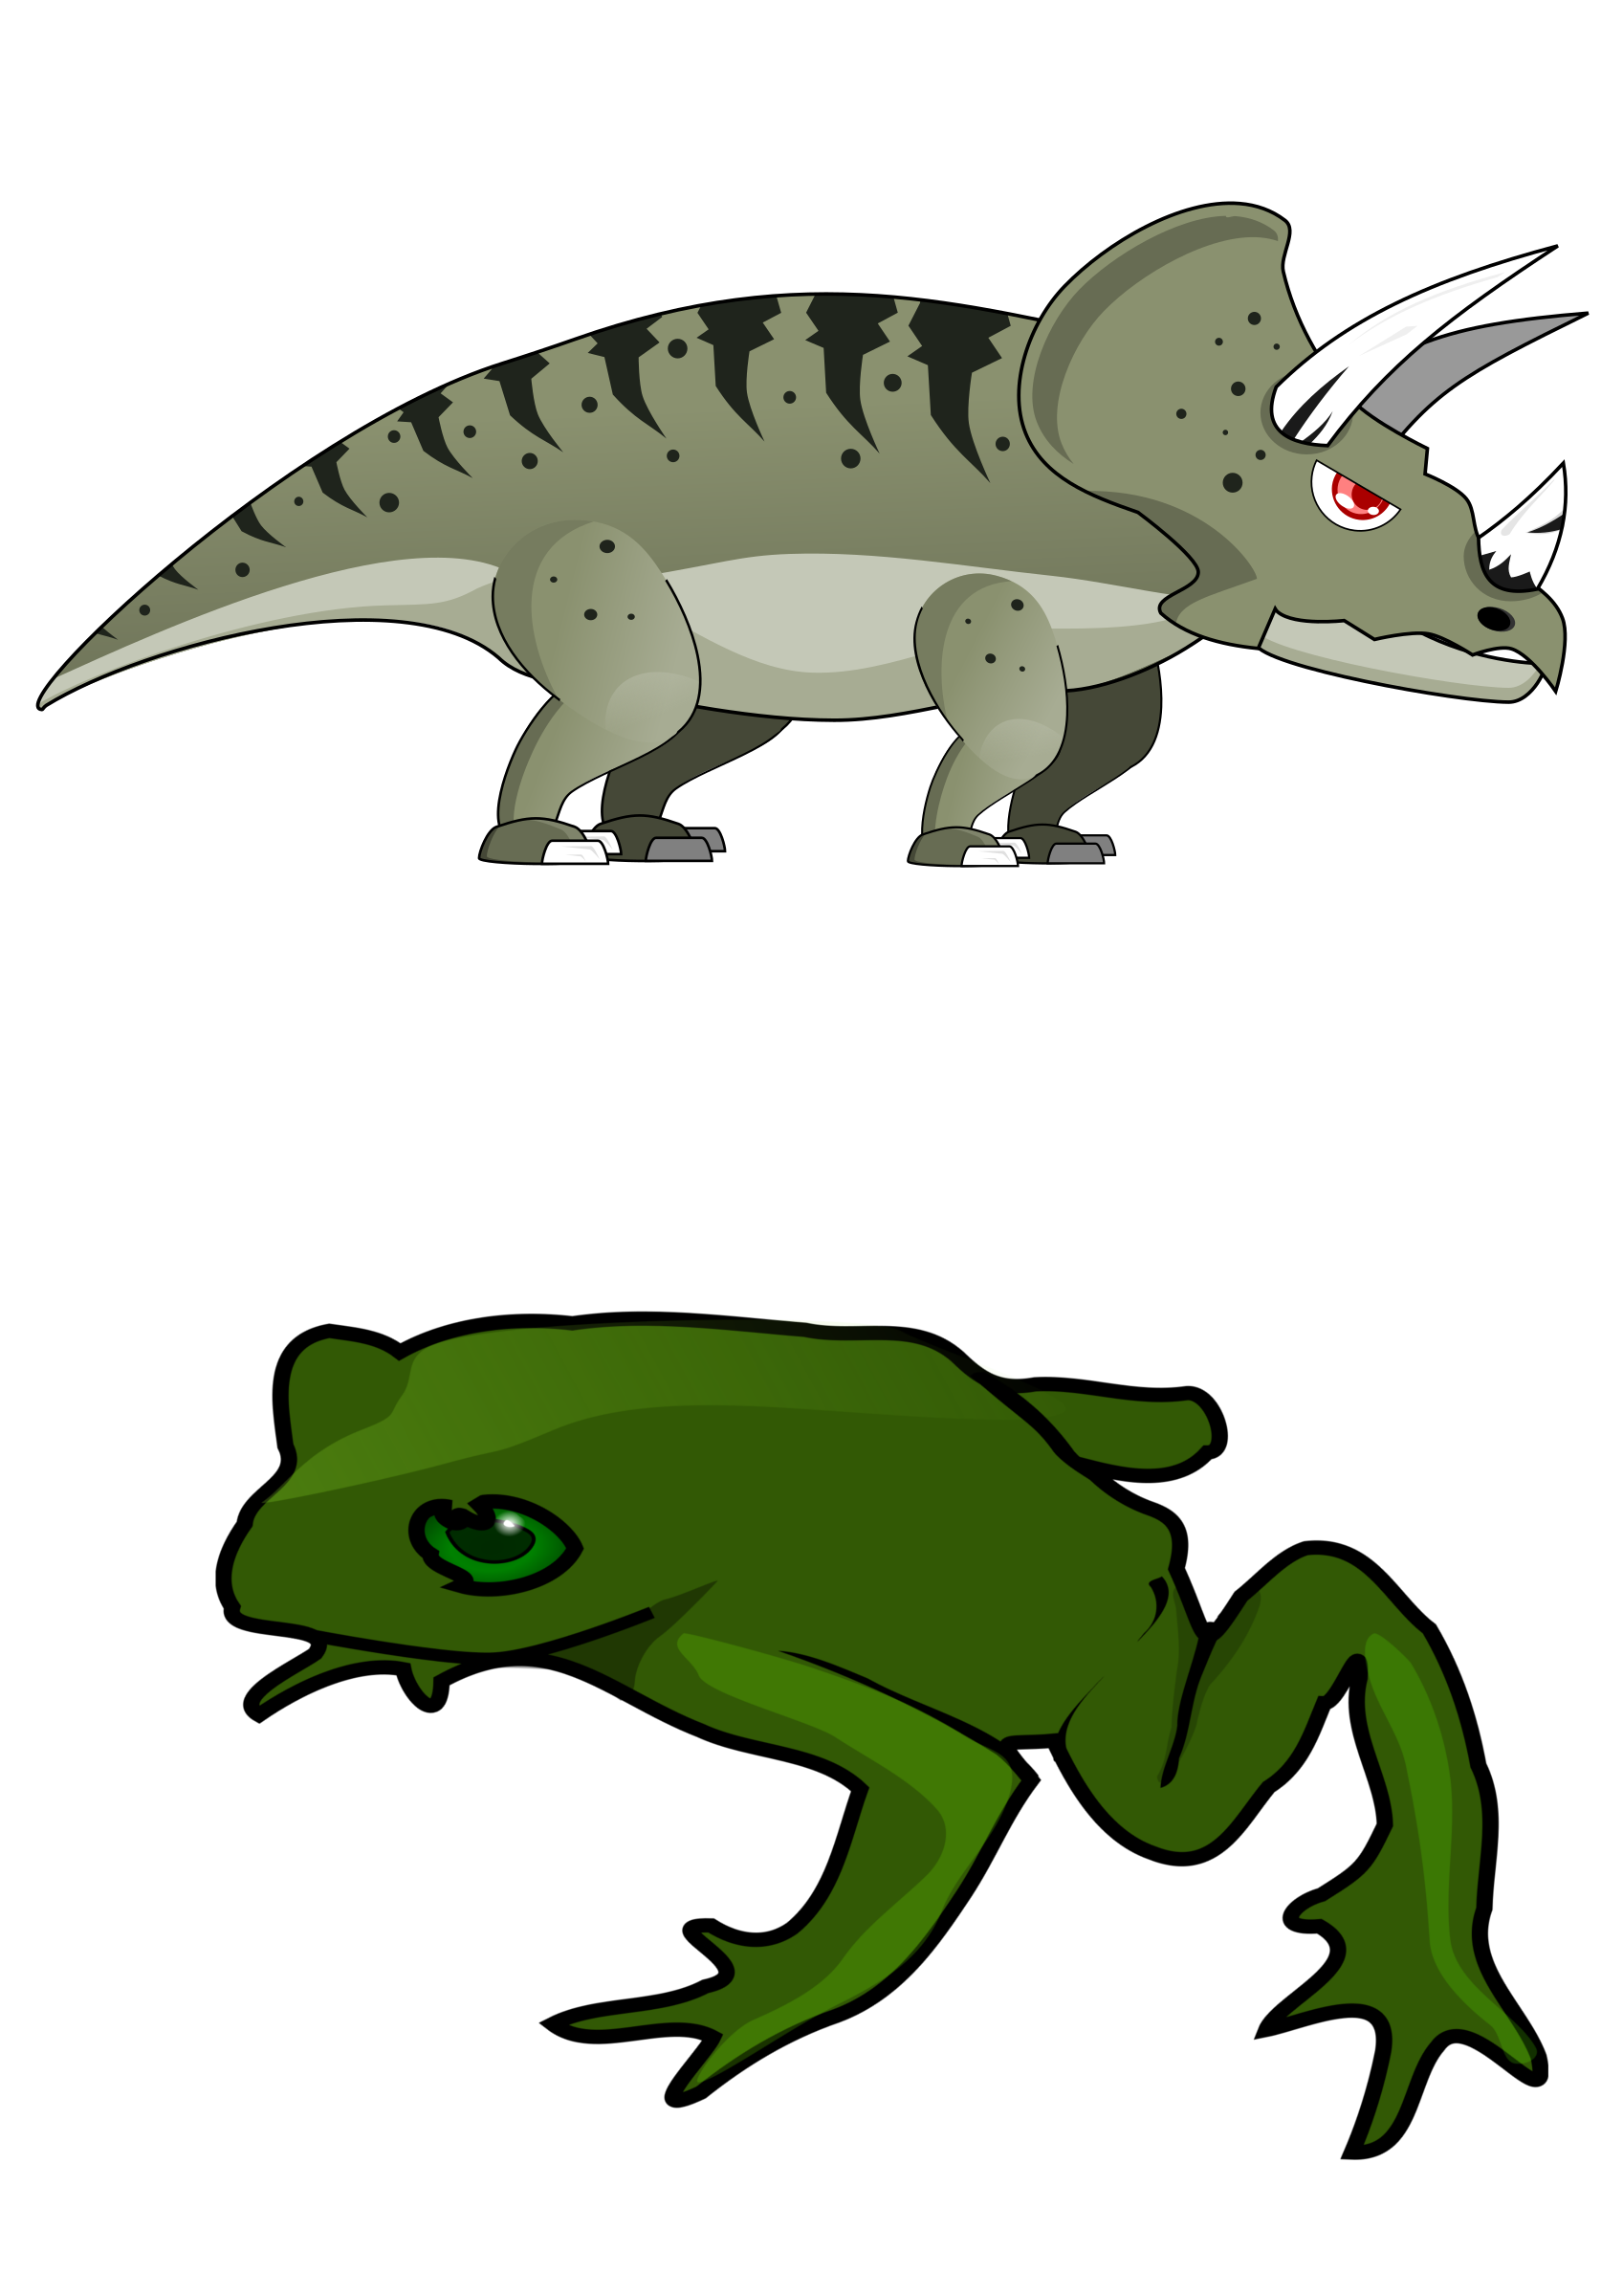
\includegraphics[width=\linewidth]{frogdinosaur.png}}
    \end{minipage} &
 \begin{minipage}{.3\textwidth}
      \uncover<4->{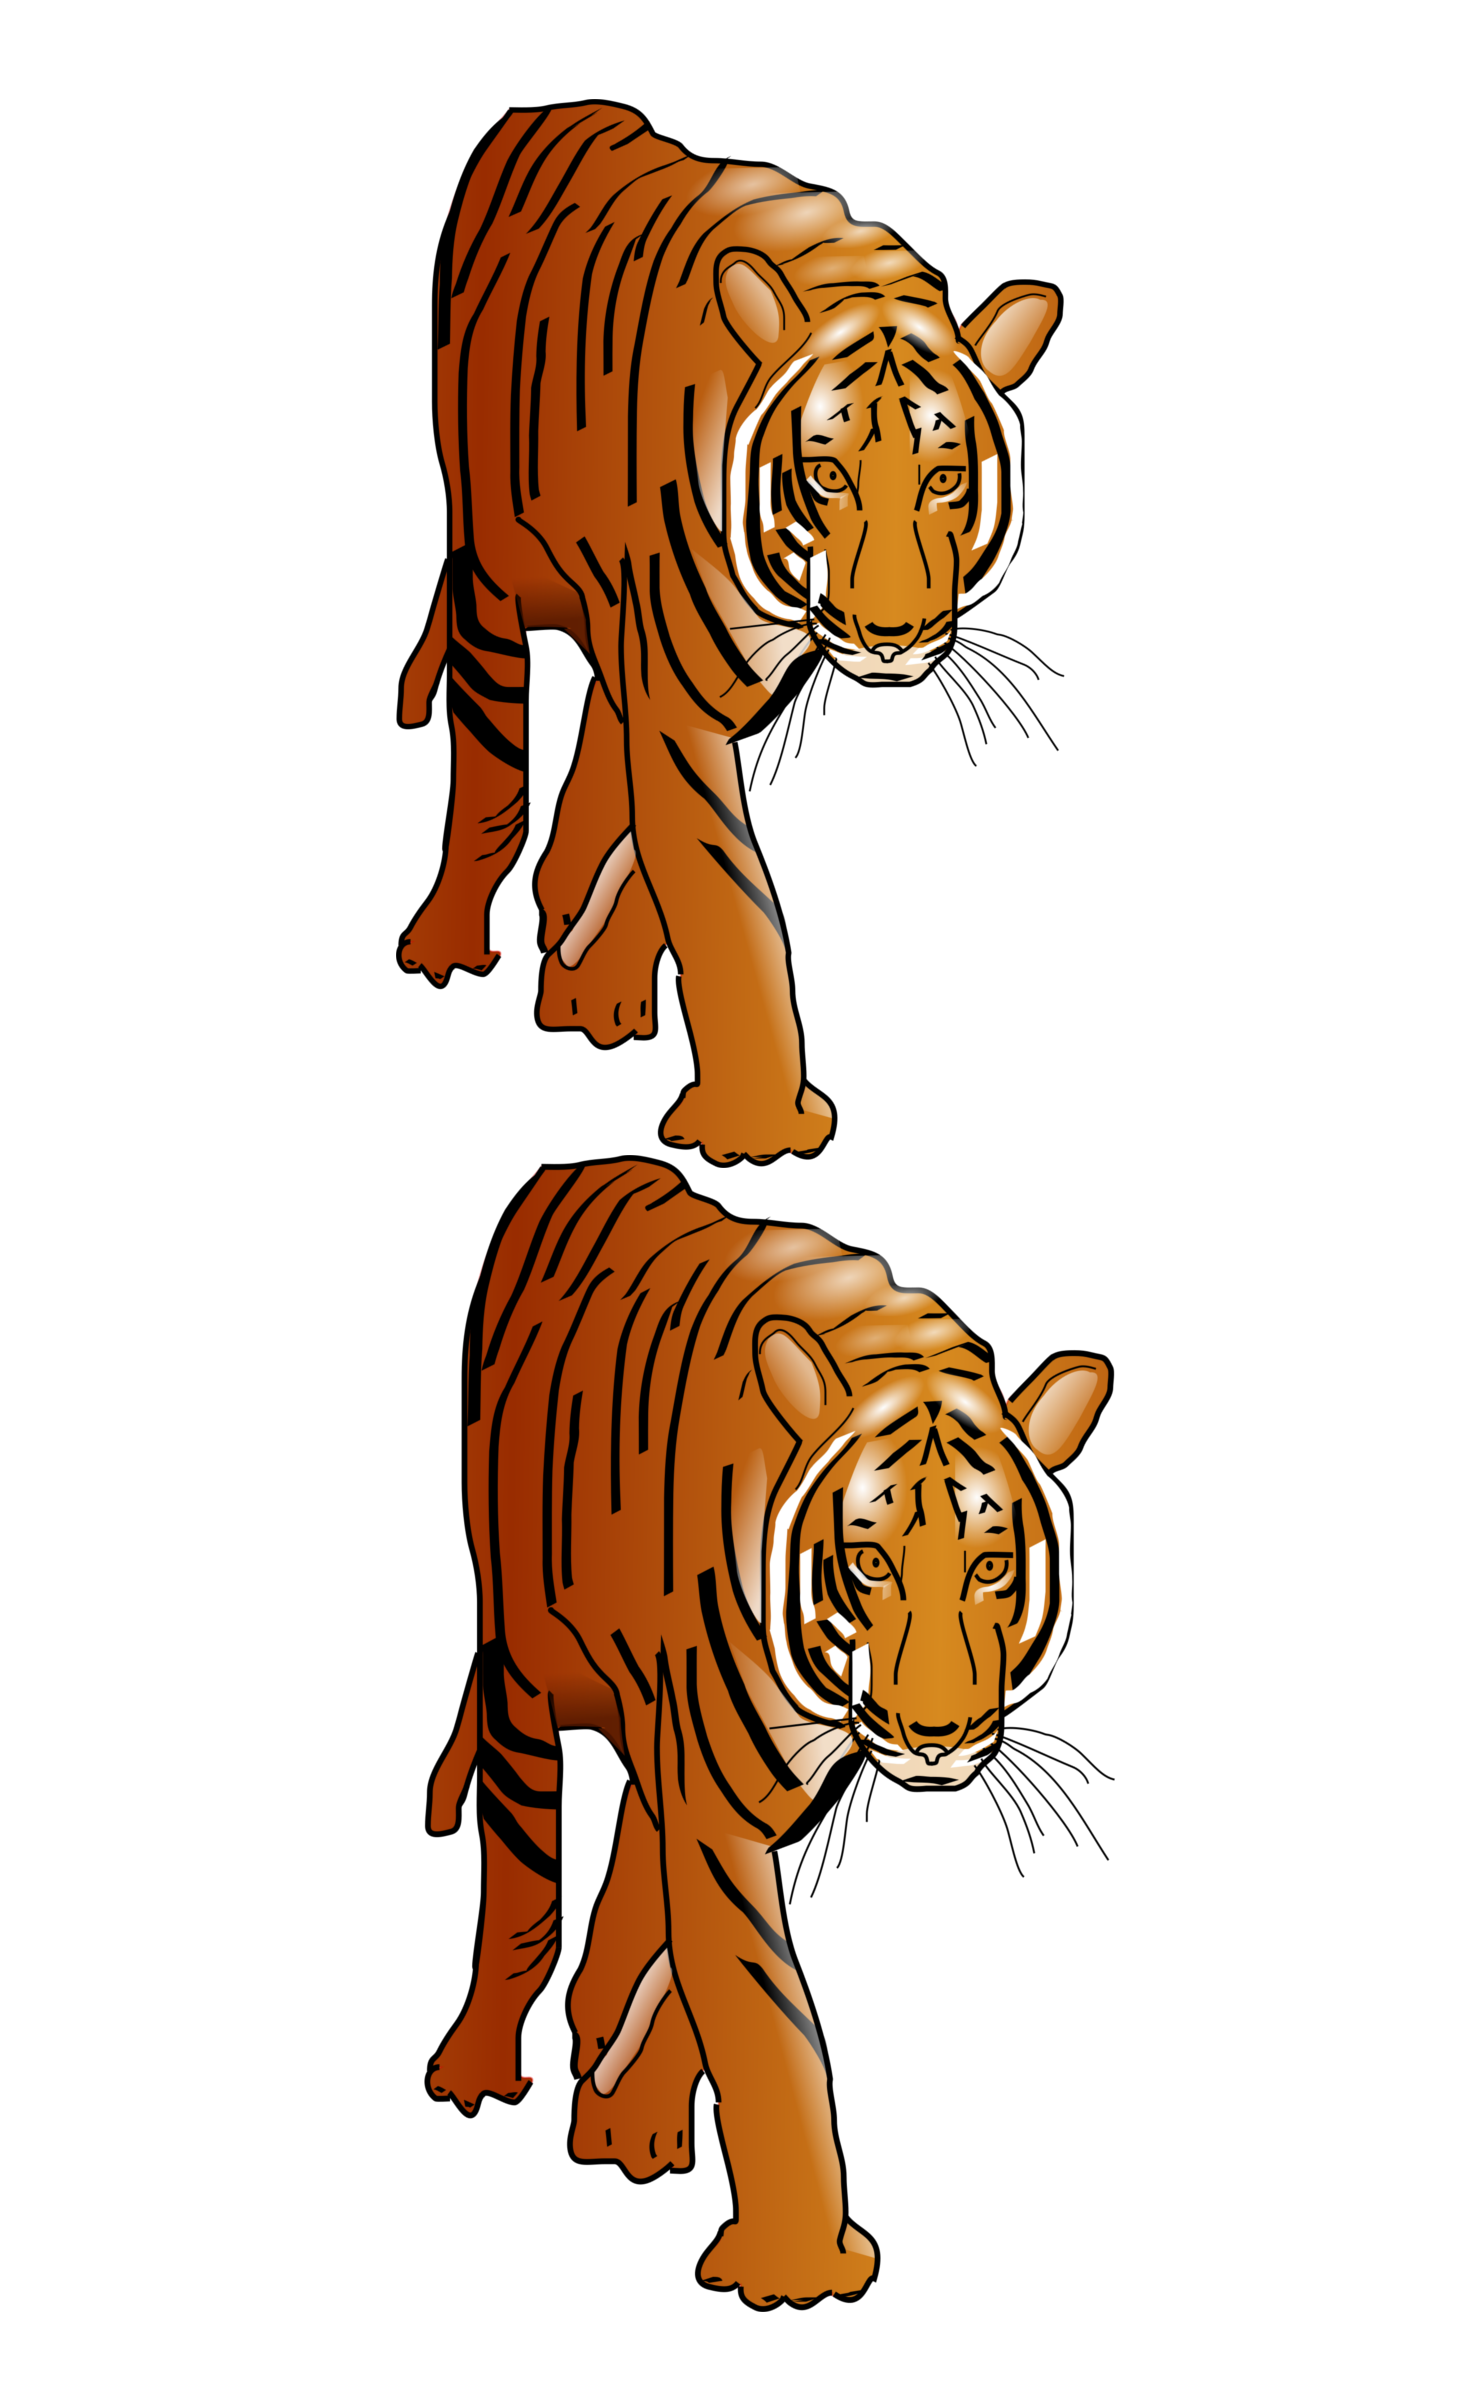
\includegraphics[width=.9\linewidth]{twotigers.png}}
    \end{minipage} & 
    \begin{minipage}{.3\textwidth}
      \uncover<6->{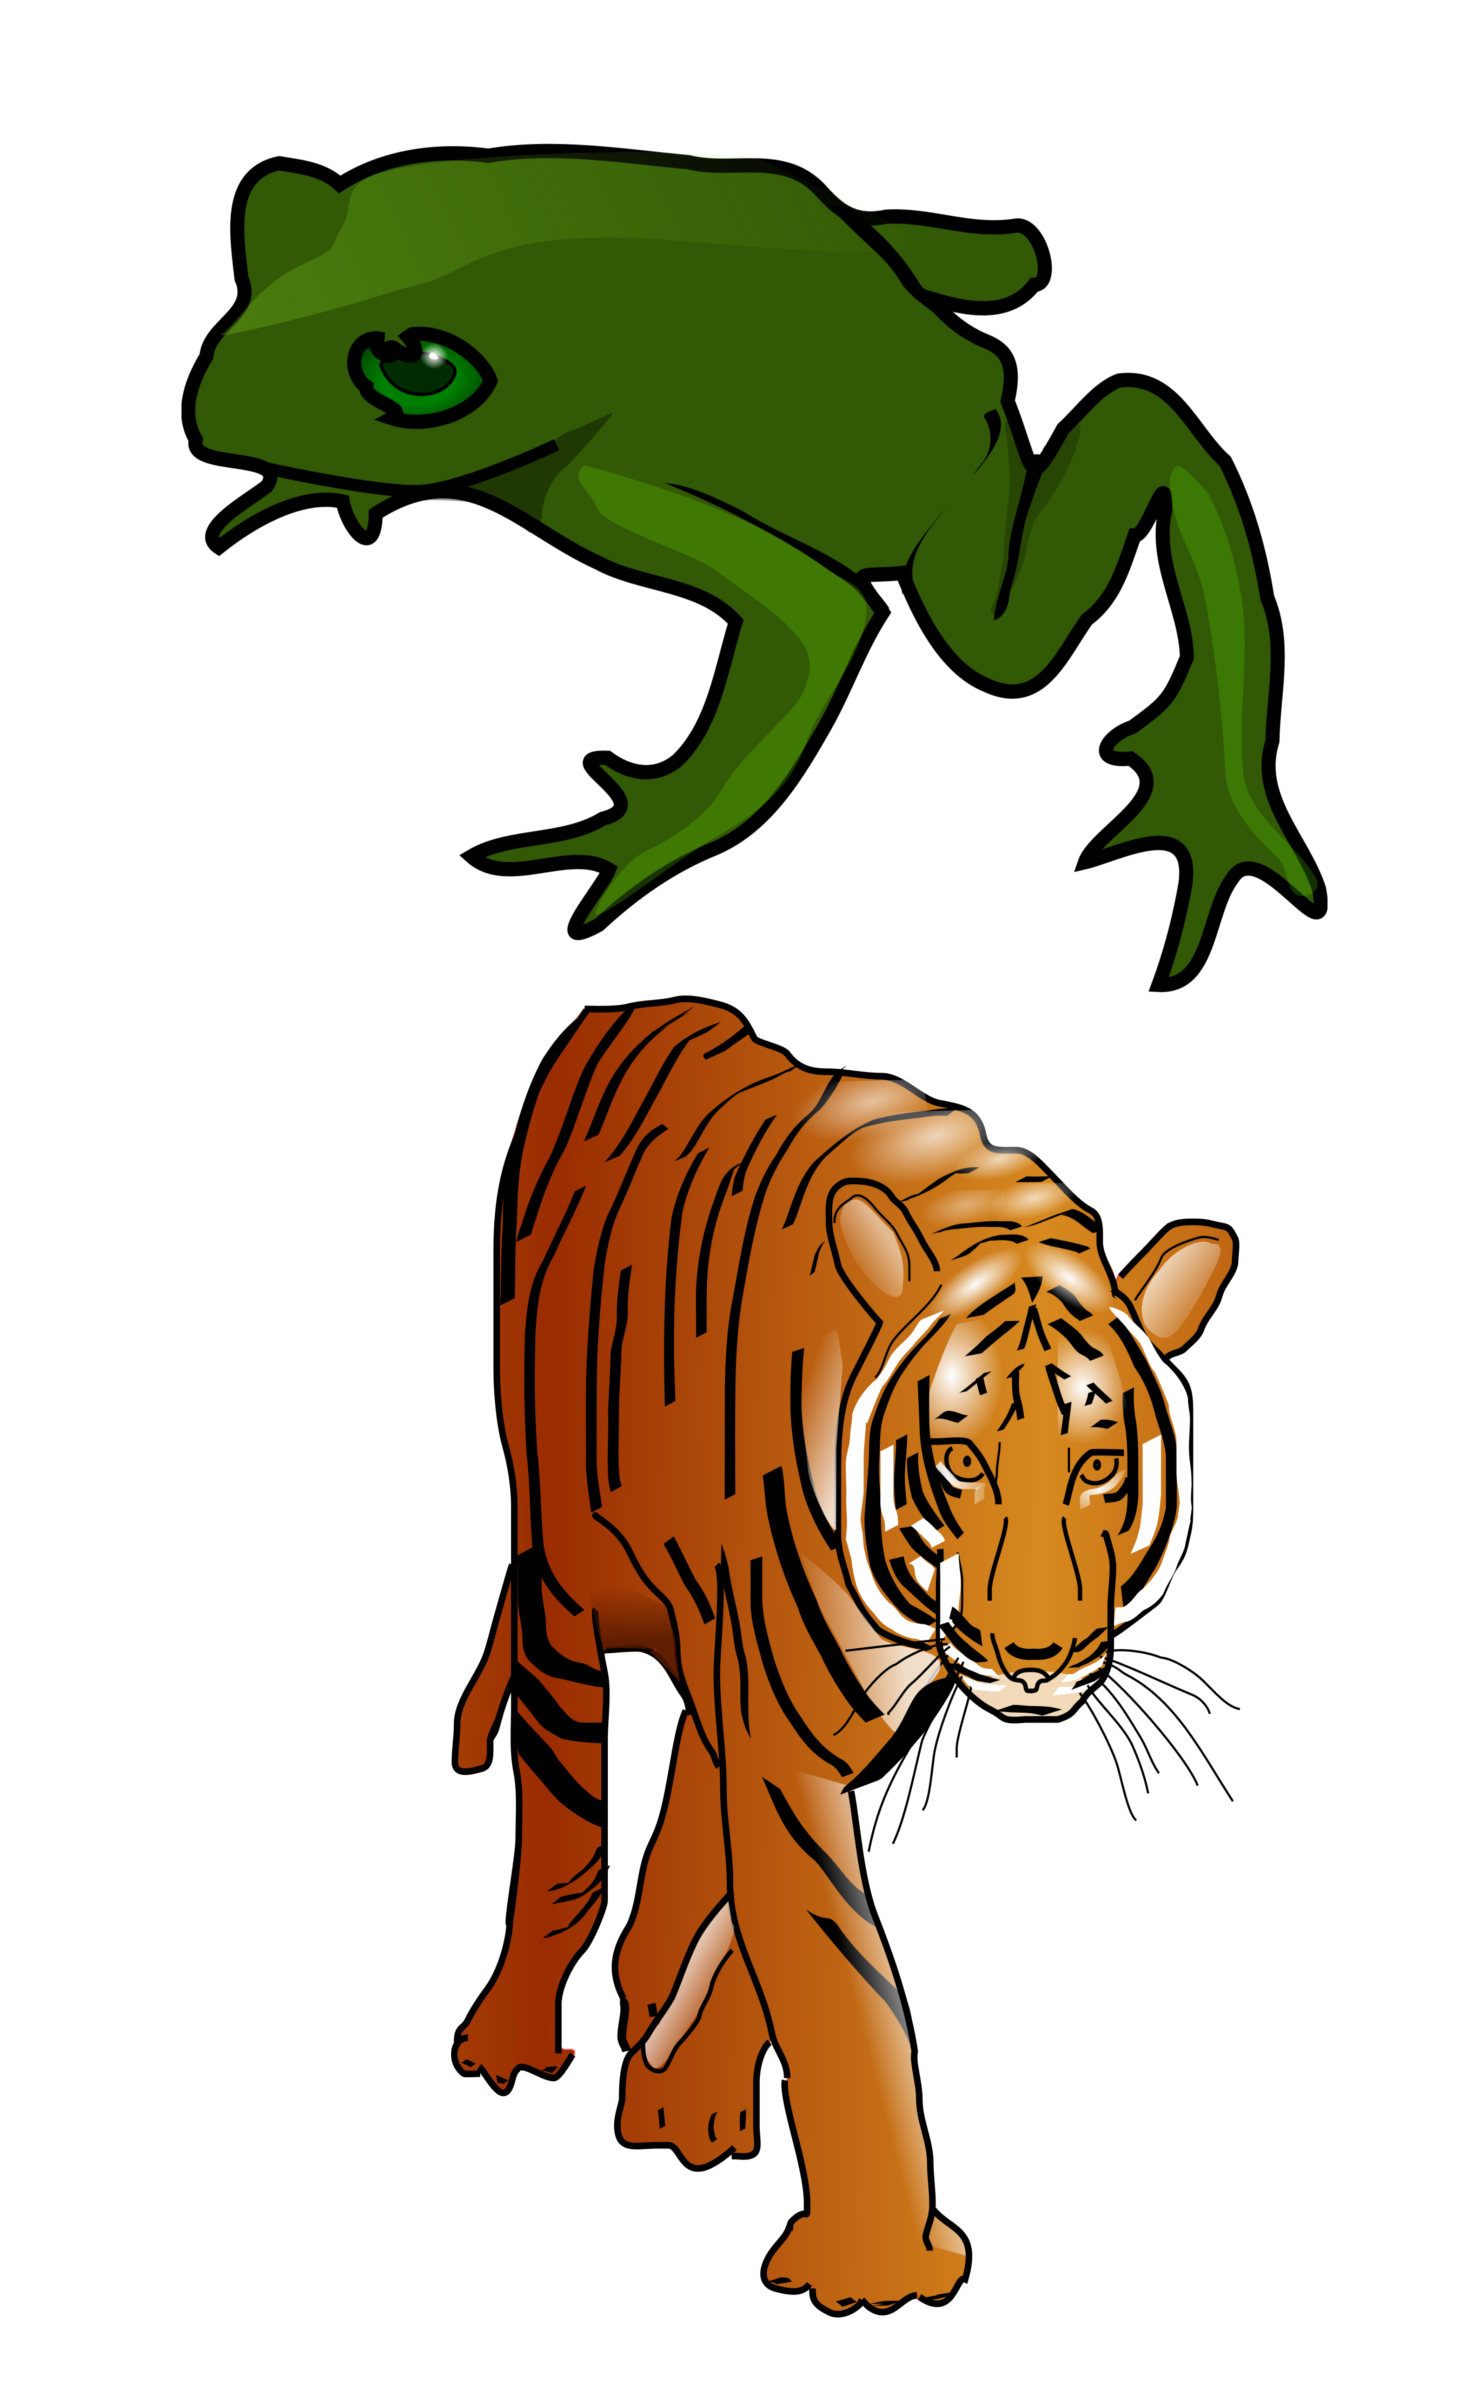
\includegraphics[width=.8\linewidth]{frogtiger.png}}
    \end{minipage} &
\uncover<8-> {$\dots$ } & 
    \begin{minipage}{.3\textwidth}
      \uncover<8->{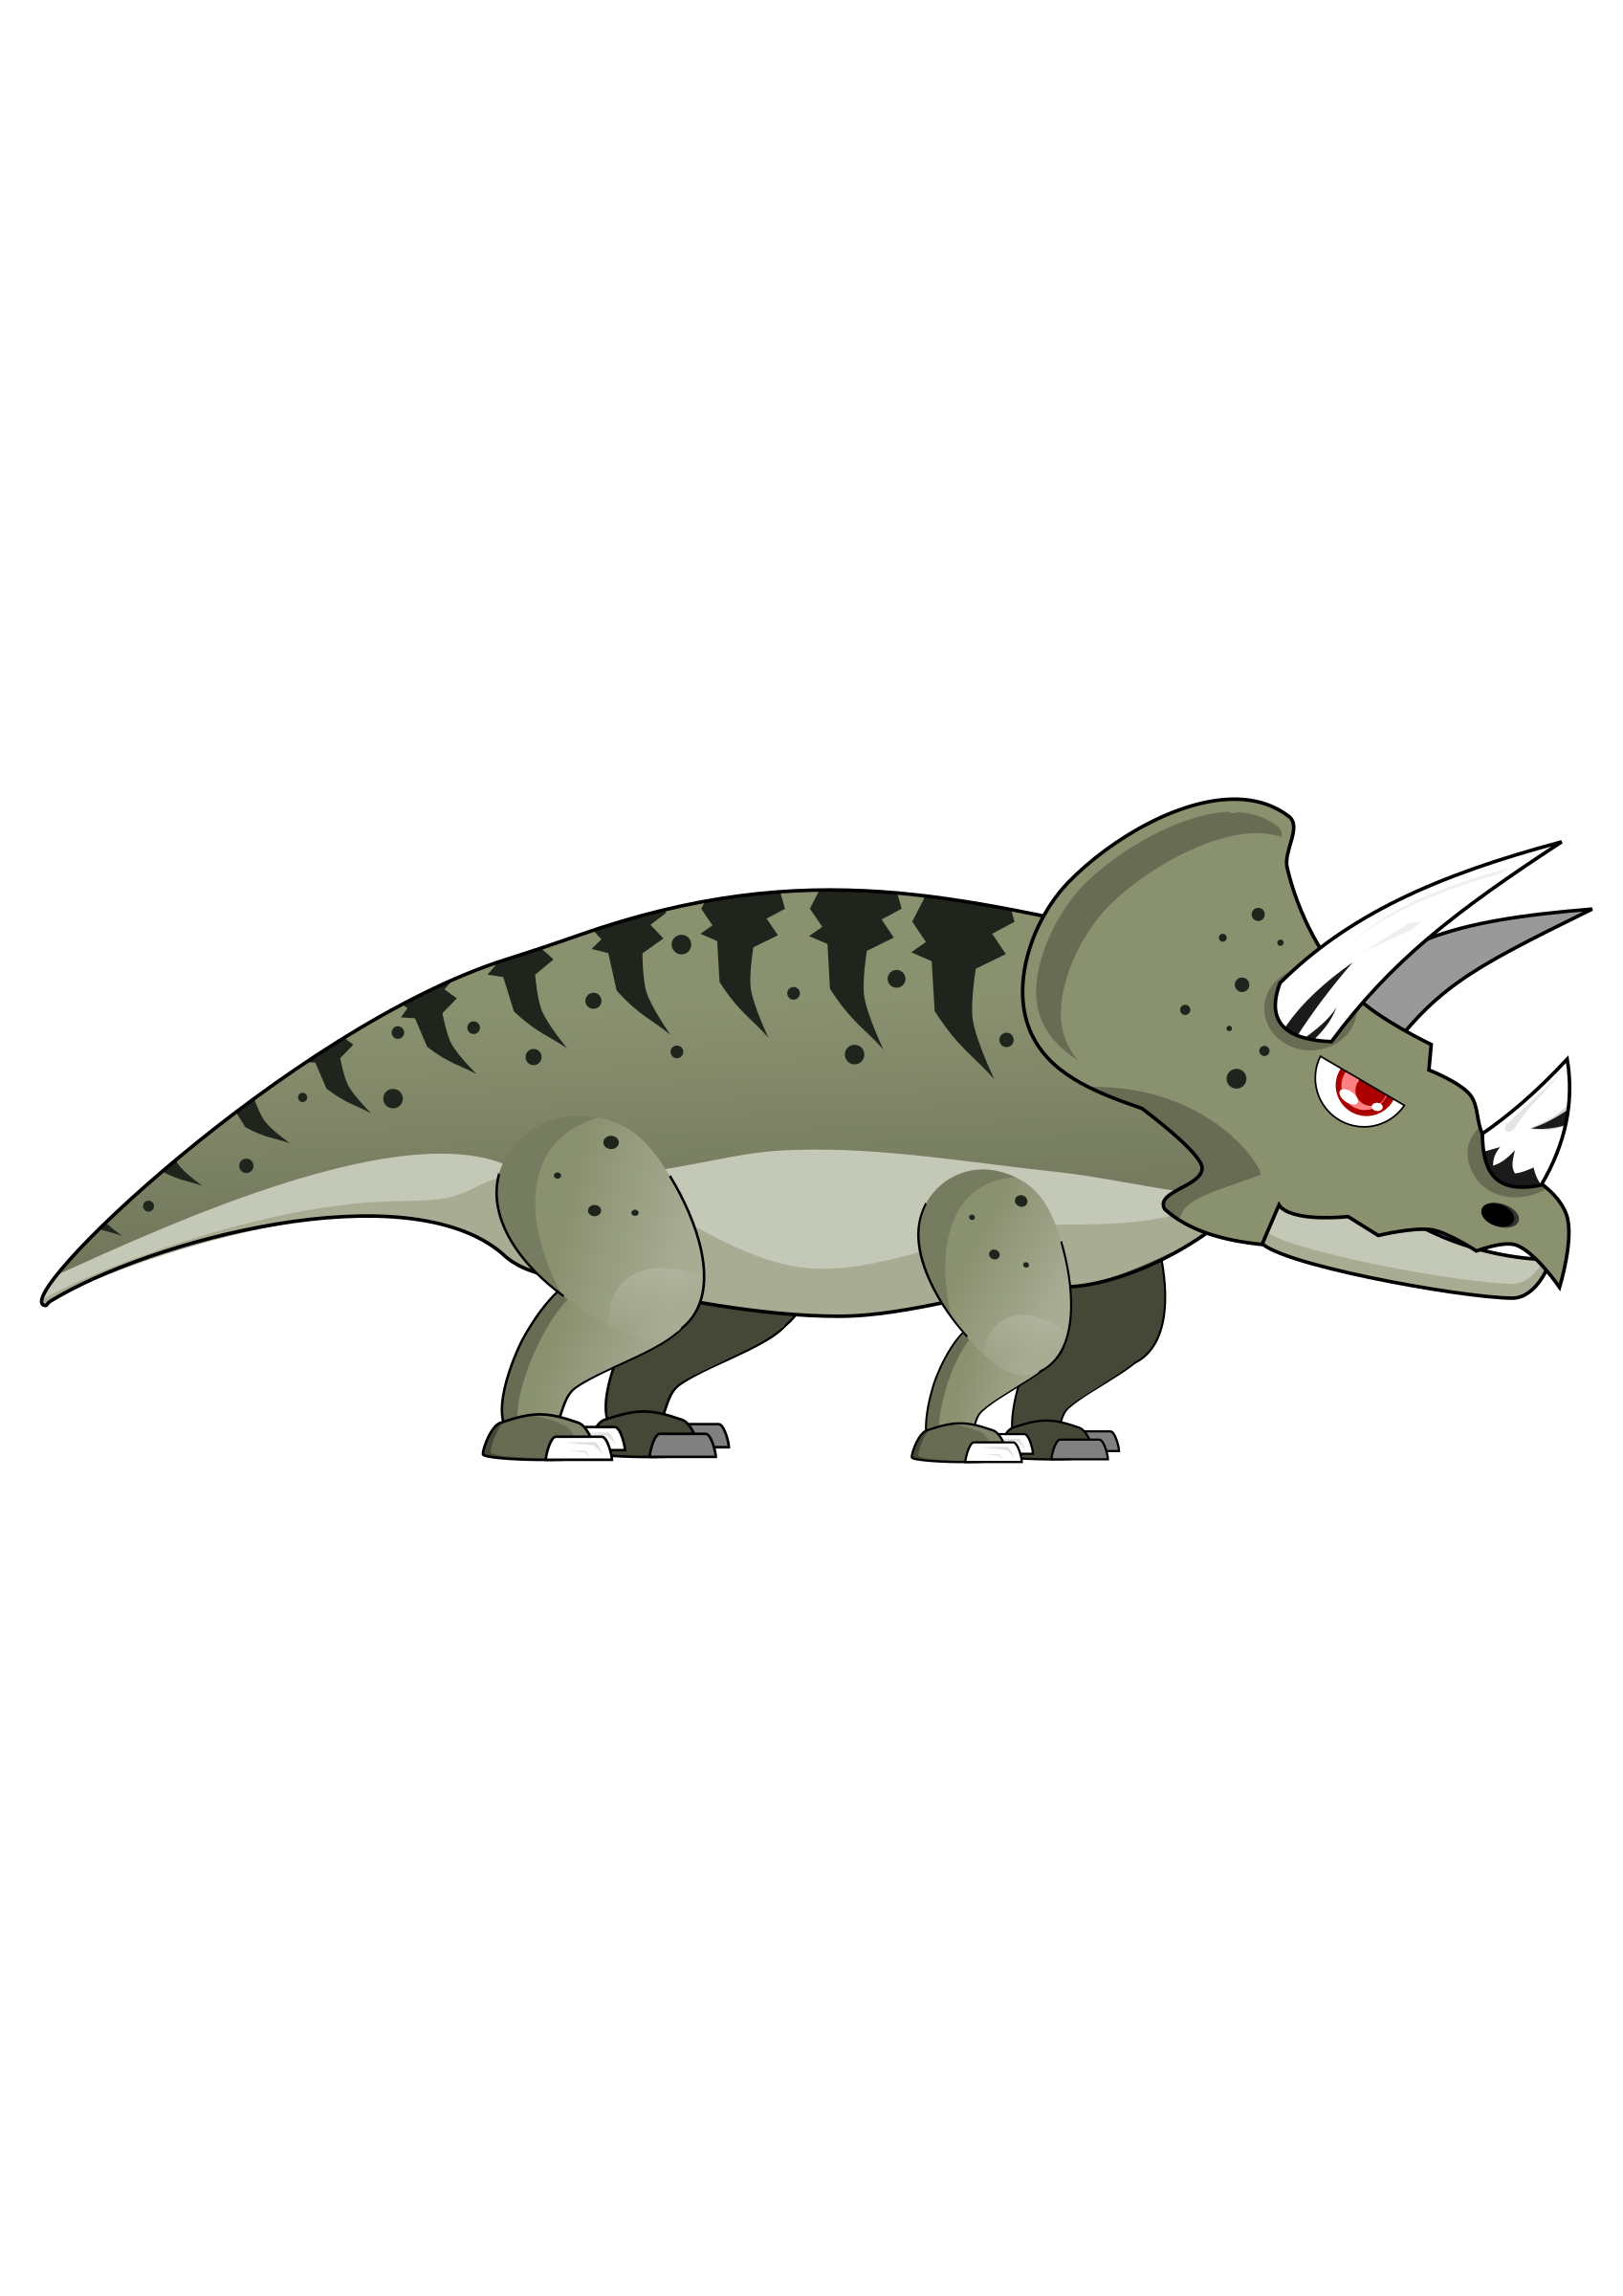
\includegraphics[width=.8\linewidth]{dinosaur2.png}}
    \end{minipage}
\\
\uncover<1->{\textbf{Reaction :}}   & 
\begin{minipage}{.3\textwidth}
\centering
\uncover<3->{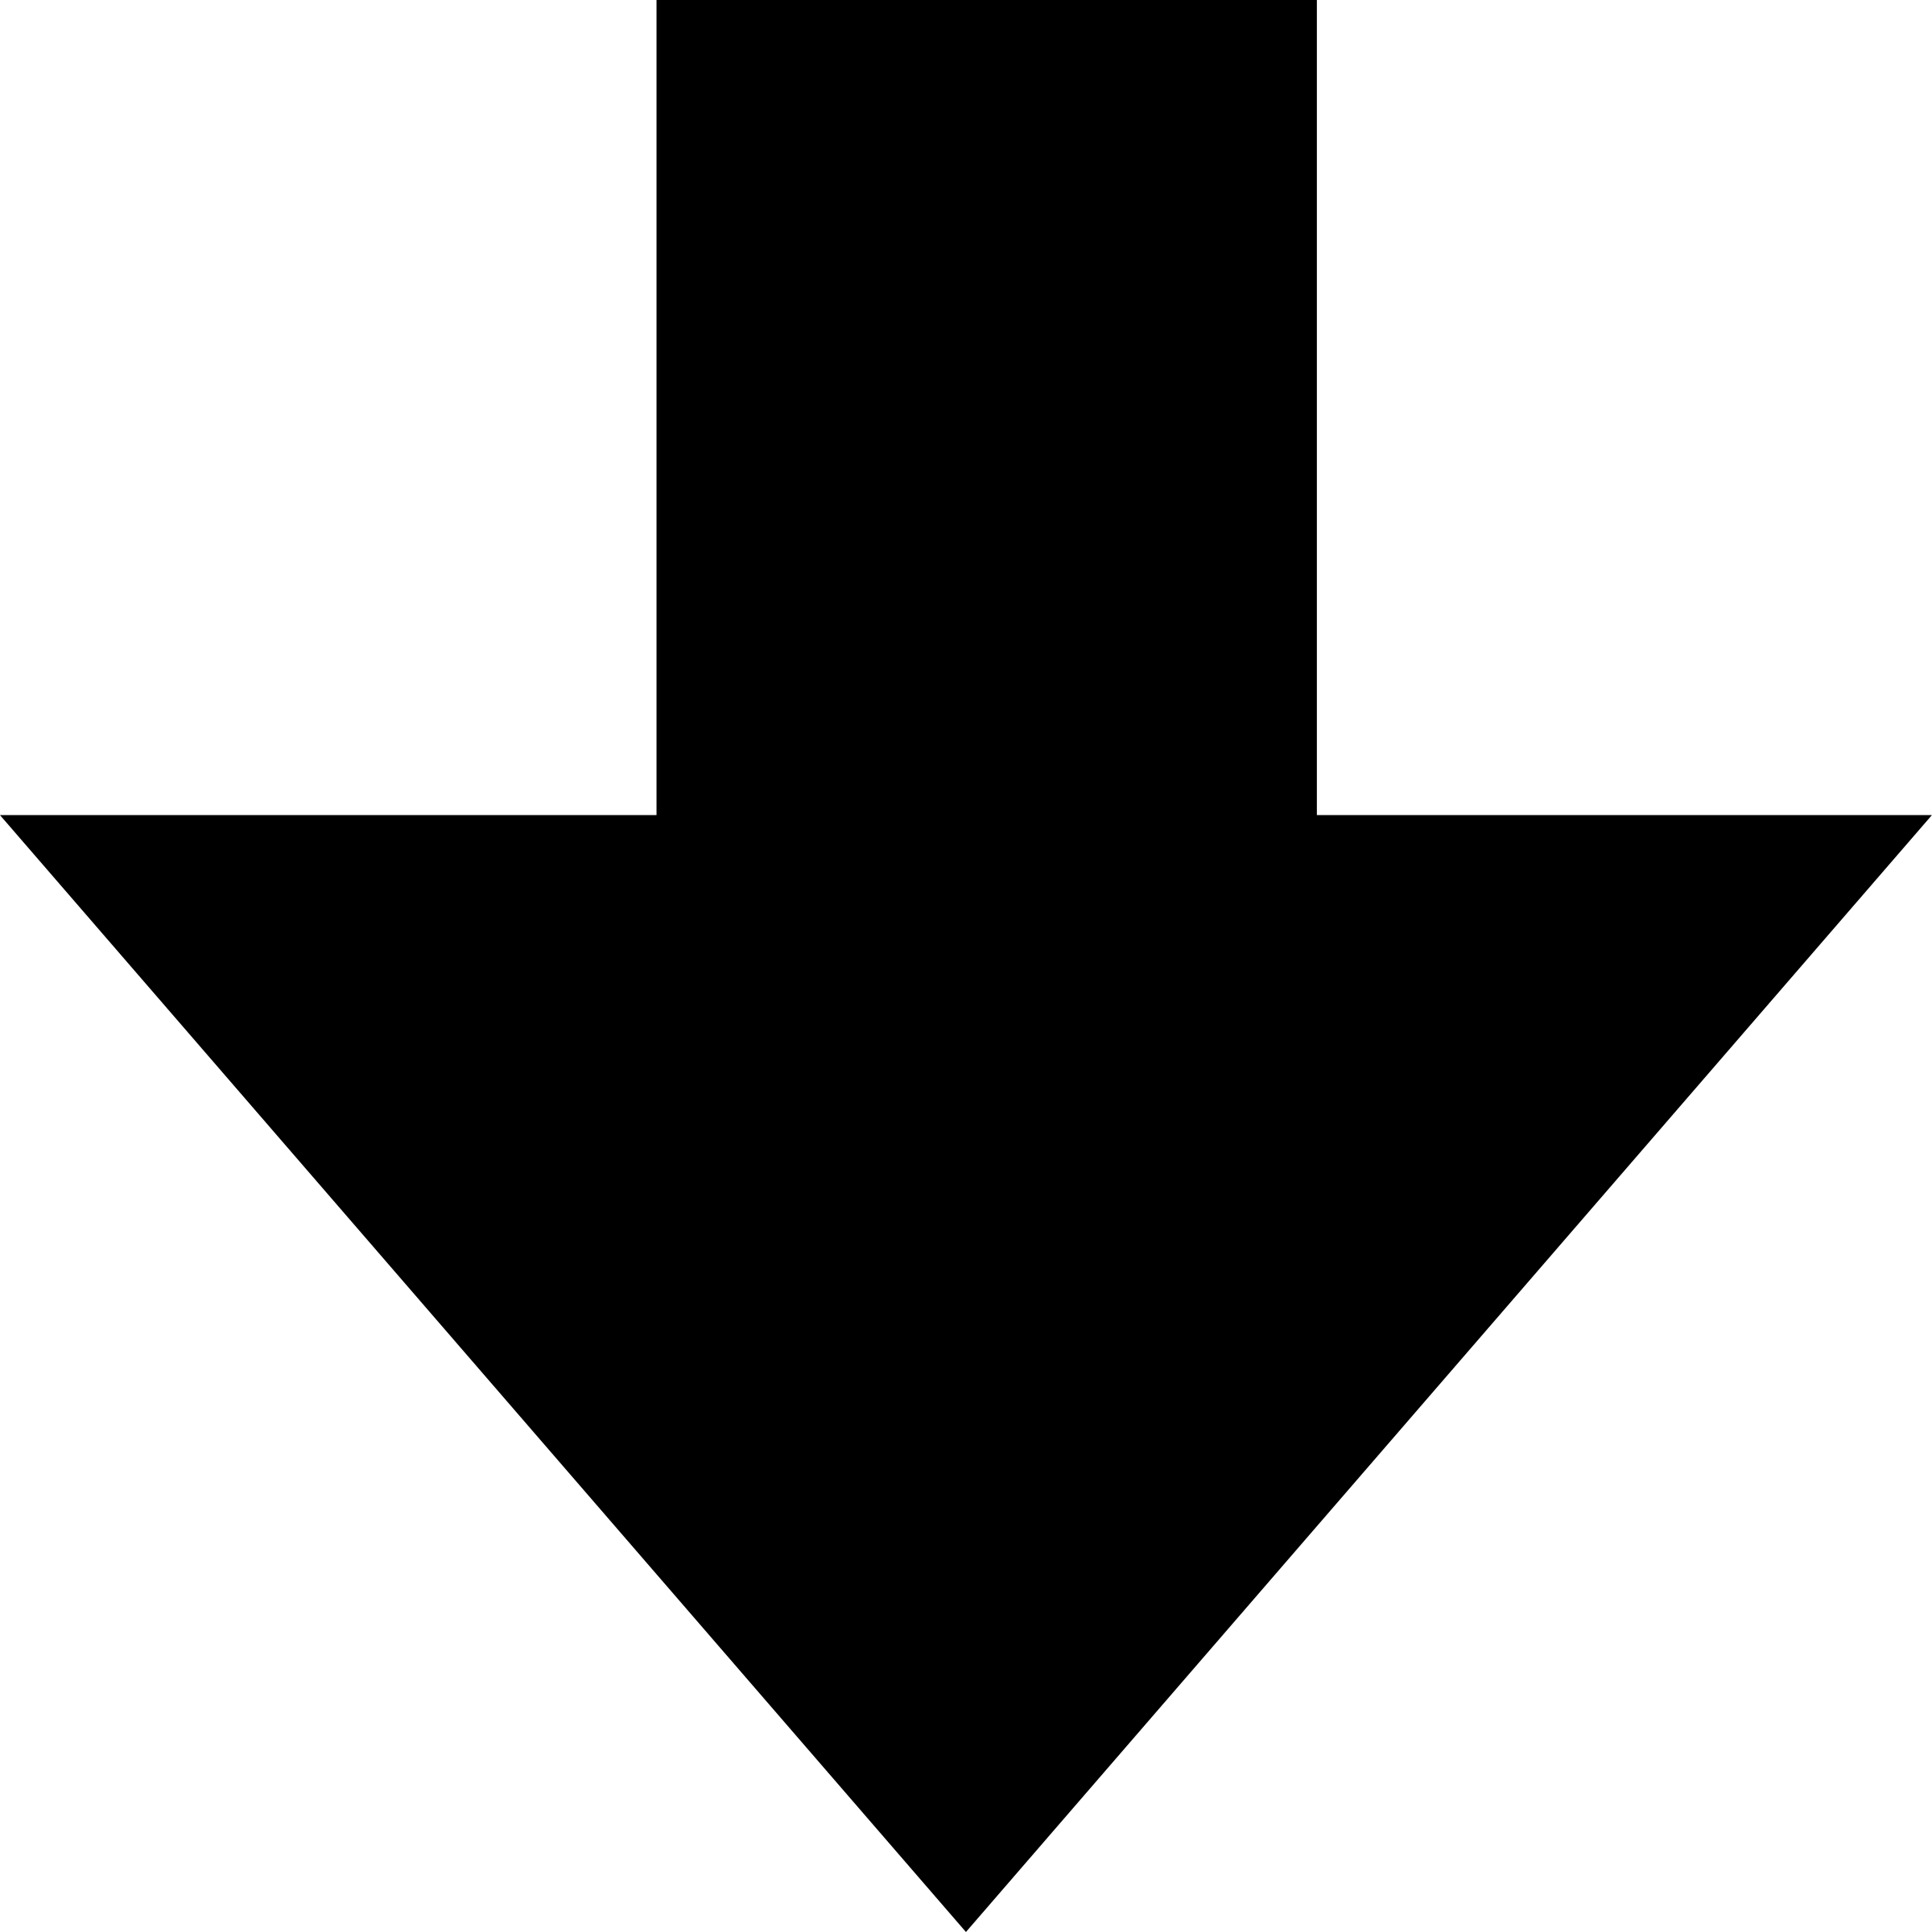
\includegraphics[width=0.2\linewidth]{downarrow.png}}
% \end{center}
    \end{minipage} 
  &     \begin{minipage}{.3\textwidth}
%       \begin{center}
\centering
\uncover<5->{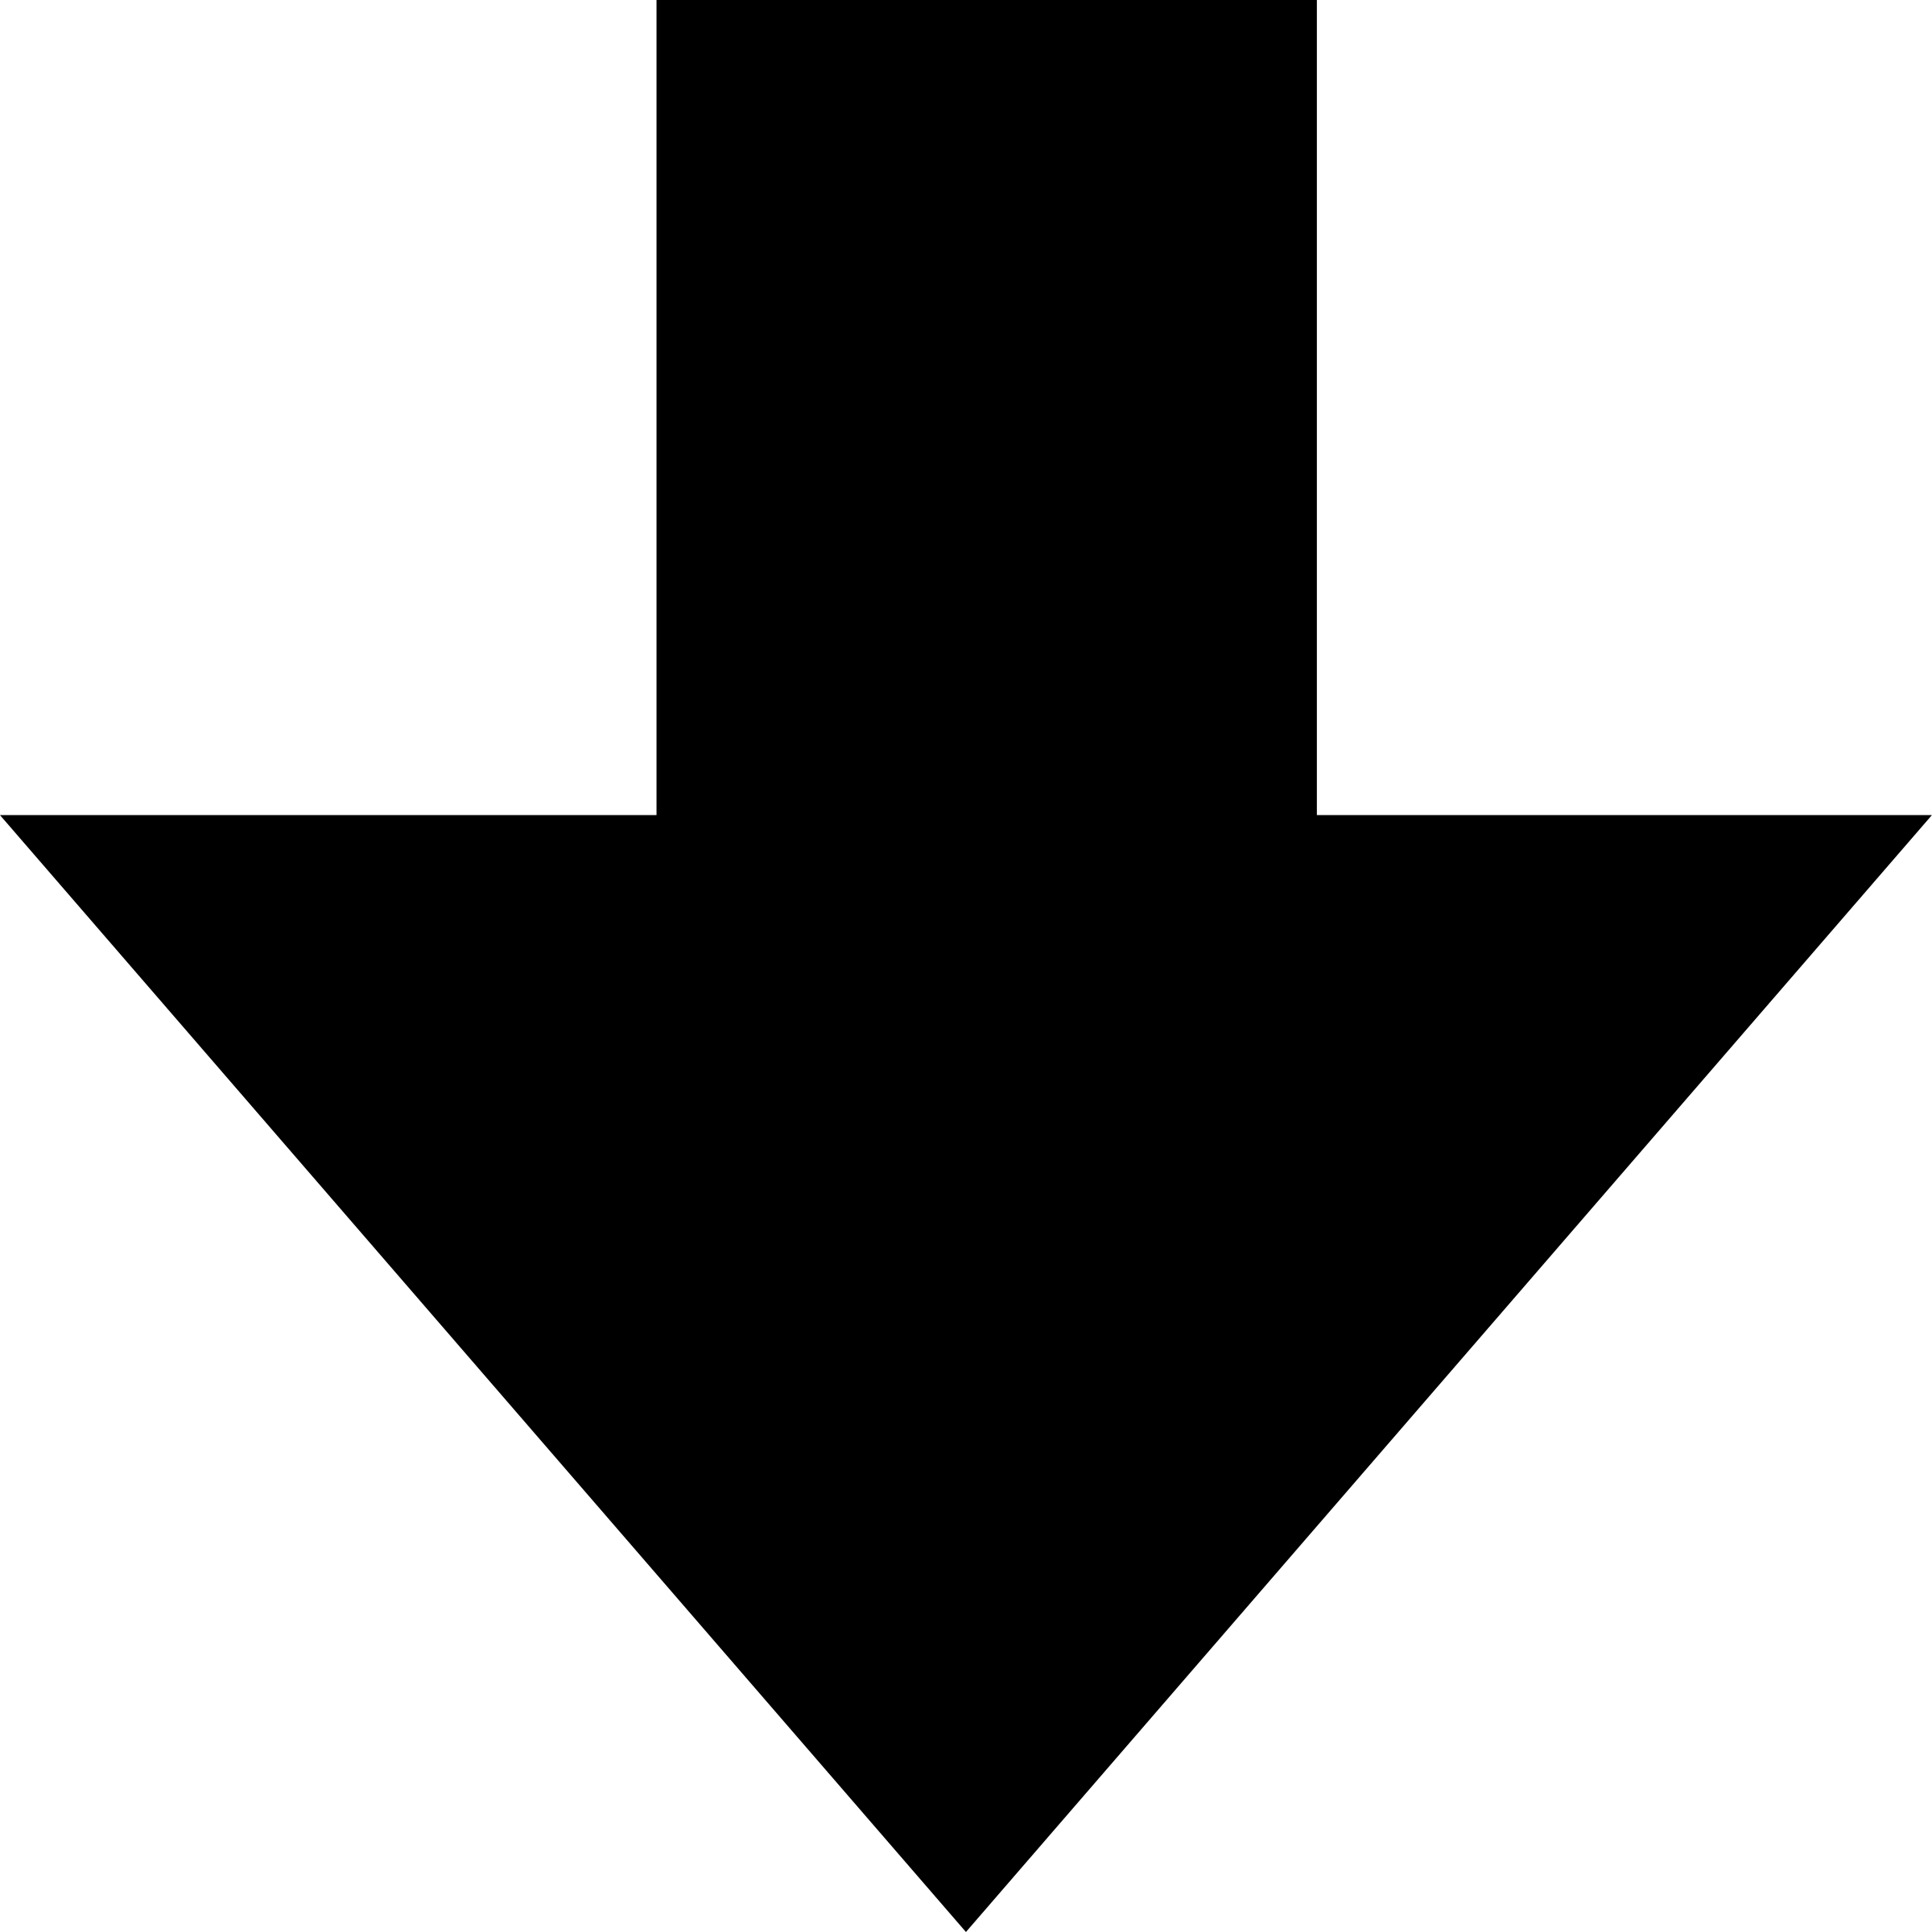
\includegraphics[width=0.2\linewidth]{downarrow.png}}
% \end{center}
    \end{minipage} 
  
% \begin{center}
% \end{center}
&     \begin{minipage}{.3\textwidth}
\centering
\uncover<7->{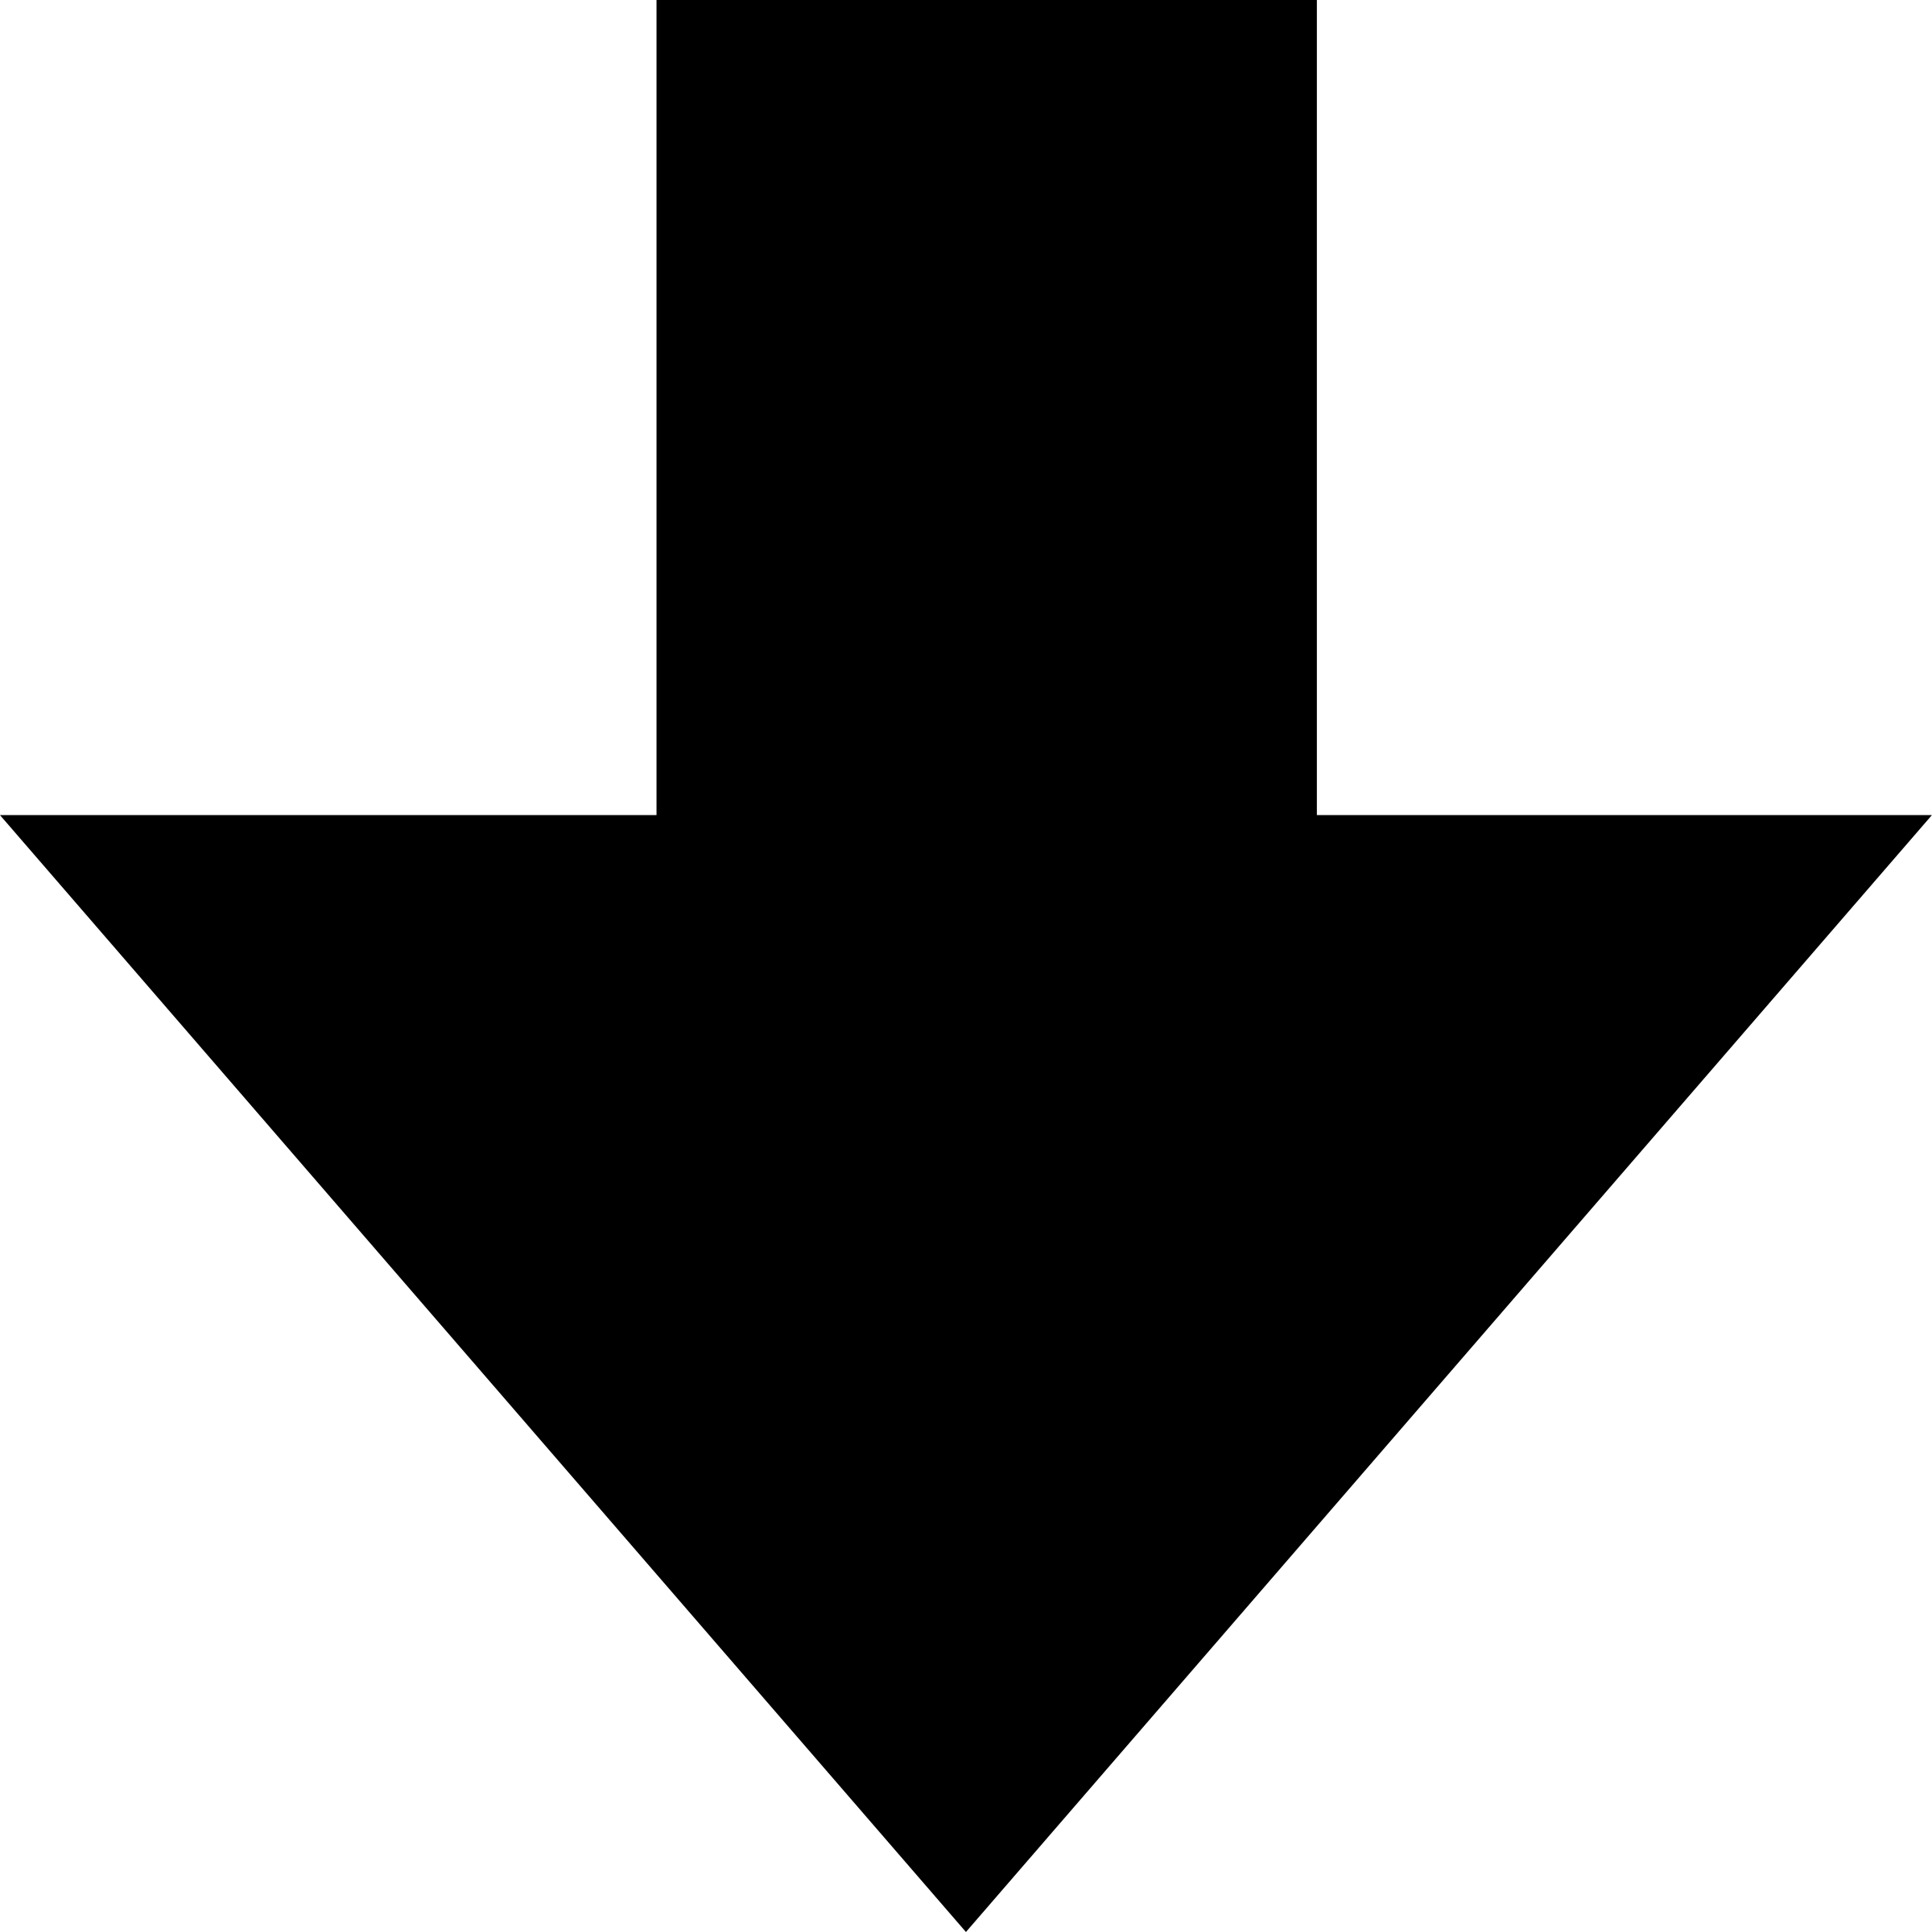
\includegraphics[width=0.2\linewidth]{downarrow.png}} 
% \end{center}
    \end{minipage} 
&
% \centering
\uncover<9->{$\vdots$}
&
\begin{minipage}{.3\textwidth}
\centering
\uncover<9->{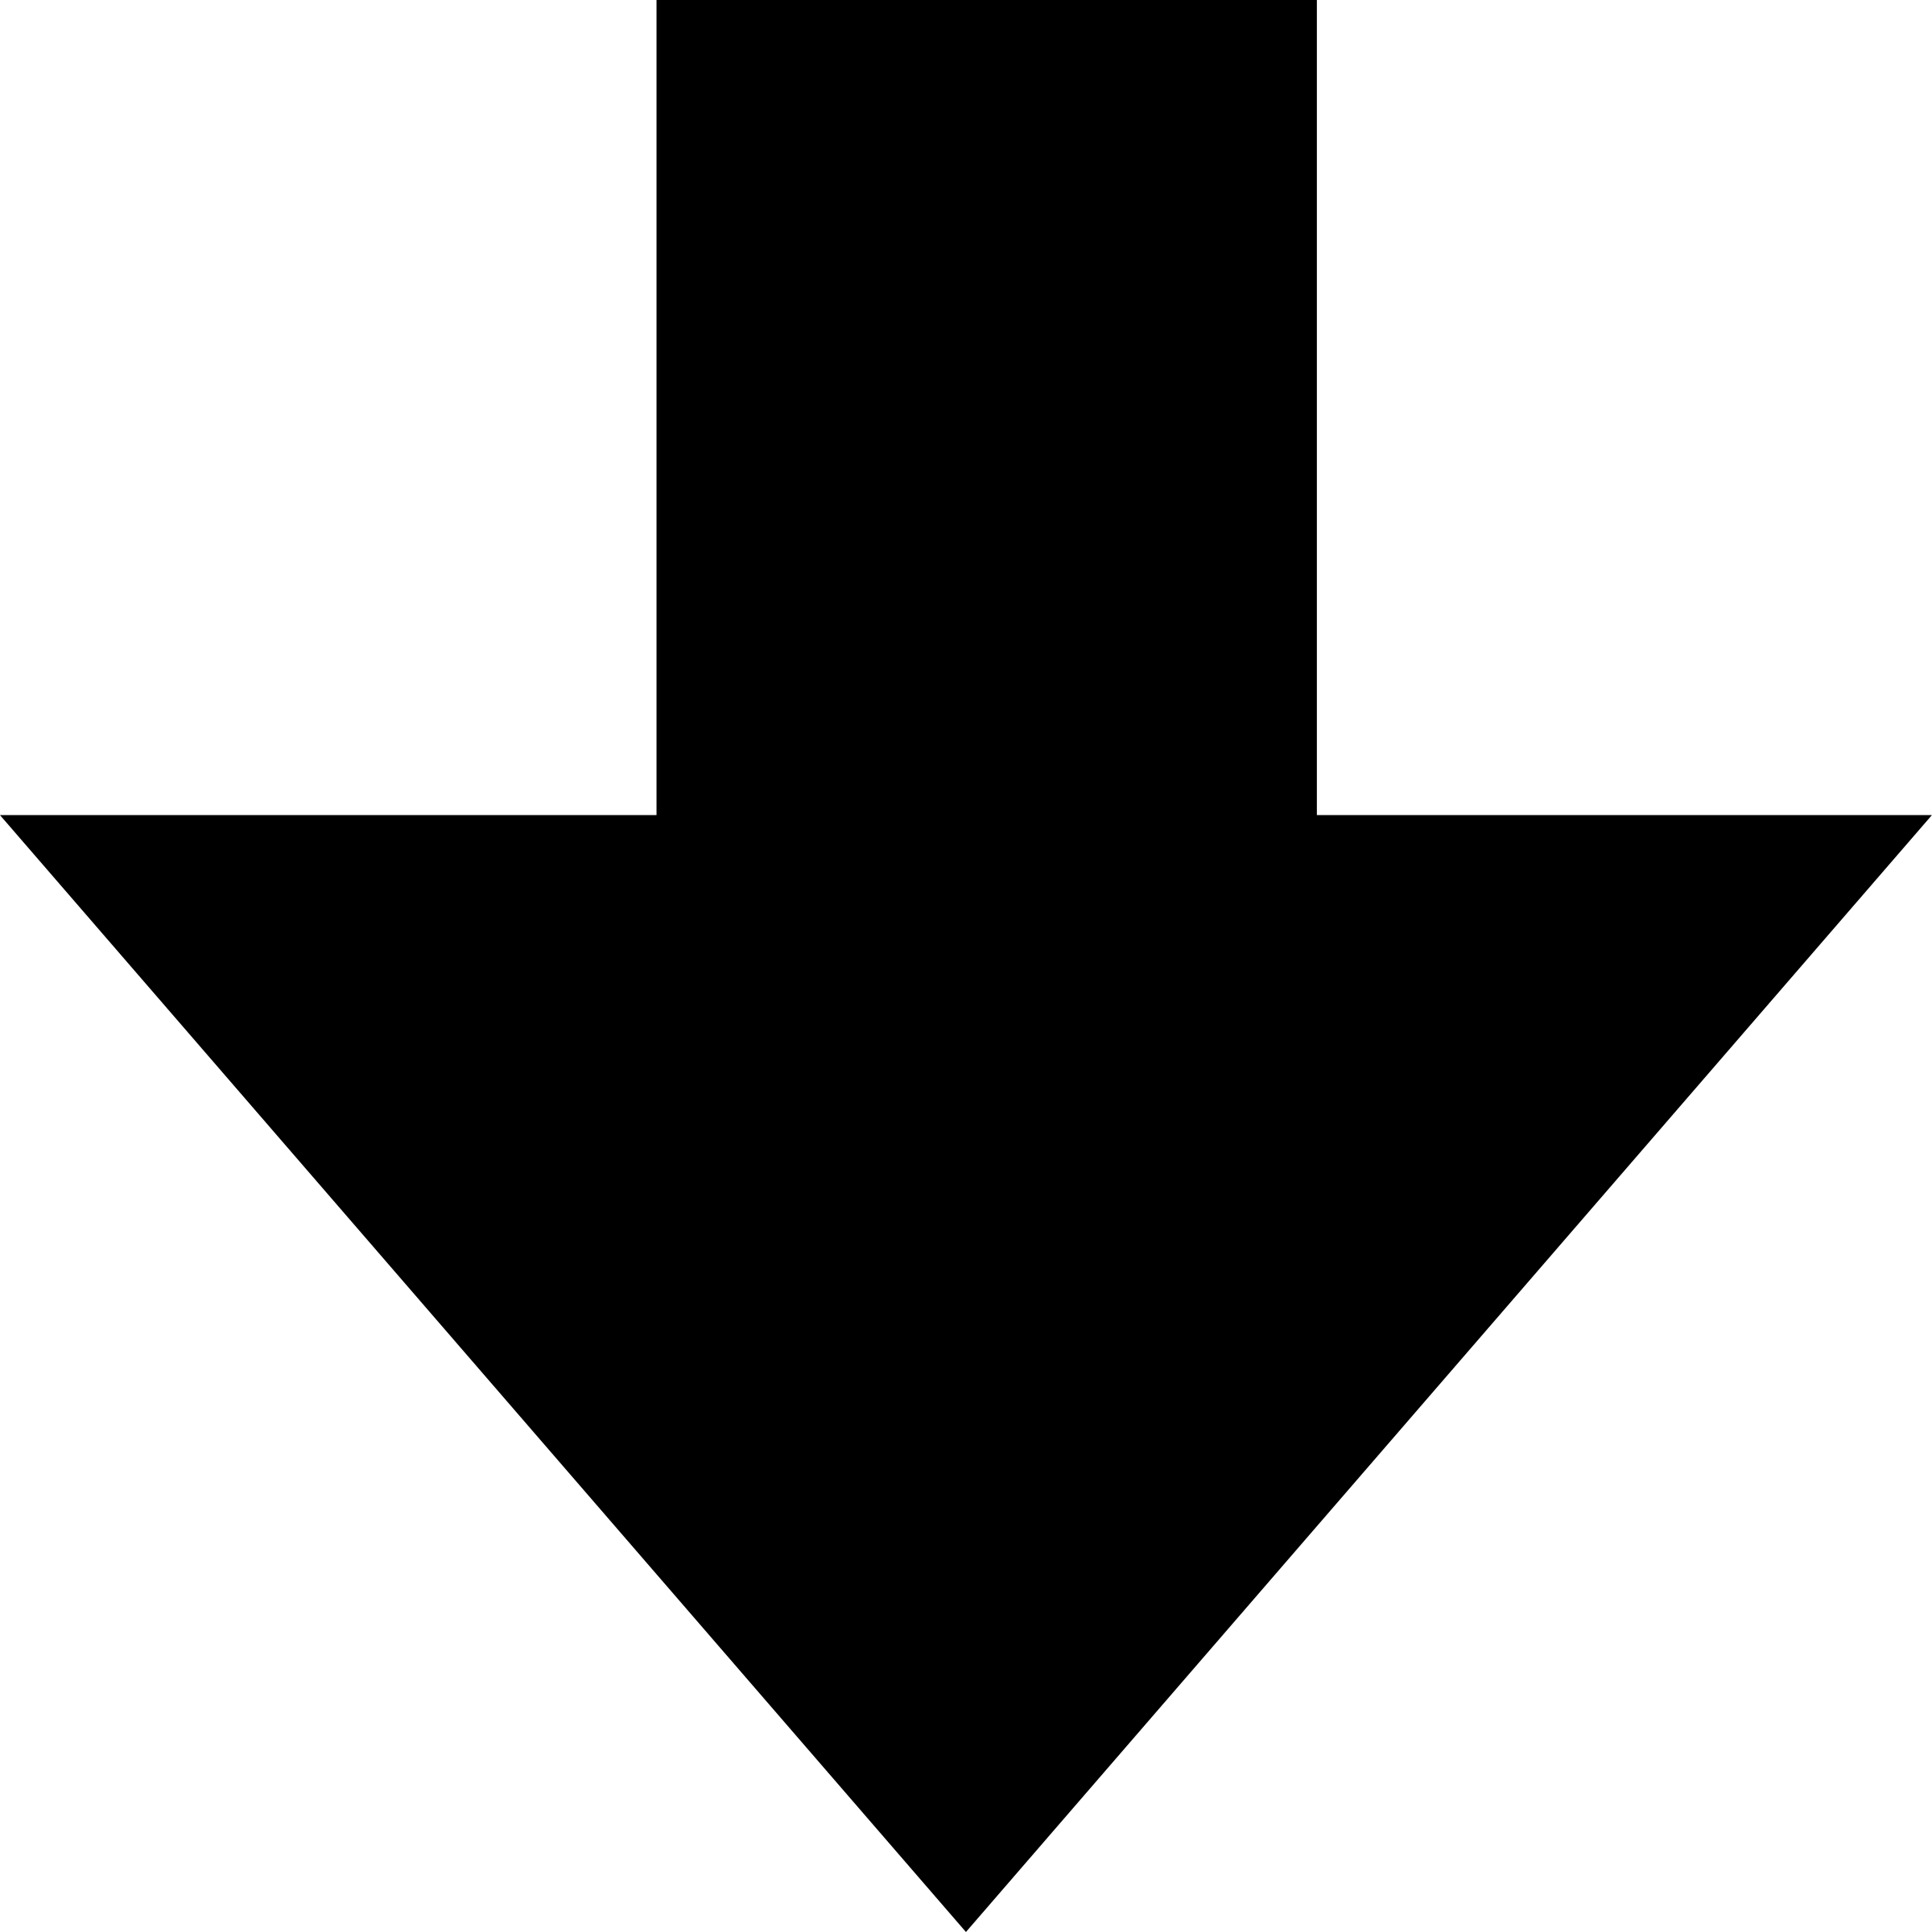
\includegraphics[width=0.2\linewidth]{downarrow.png}} 
% \end{center}
    \end{minipage} 
 \\
 & 
    \begin{minipage}{.3\textwidth}
      \onslide<3->
\includegraphics[width=0.7\linewidth]{dinosaur.png}
    \end{minipage} &  \begin{minipage}{.3\textwidth}
      \uncover<5->{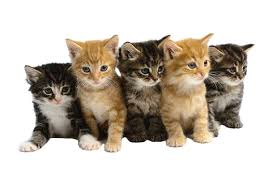
\includegraphics[width=\linewidth]{kittenscute.jpeg}}
    \end{minipage} &  
    \begin{minipage}{.3\textwidth}
      \uncover<7->{
\includegraphics[width=.6\linewidth]{tiger.png}}
    \end{minipage}&
\uncover<9-> {$\dots$ }
& 
    \begin{minipage}{.3\textwidth}
      \uncover<9->{
\includegraphics[width=.6\linewidth]{extinct.png}}
    \end{minipage}
\\
\rule{0pt}{4ex}  
  \onslide<10-> \textbf{Number of Reactants:} & $h_1$ \onslide<11->$=N_1\cdot N_S$  & $h_2$\onslide<12->$=N_2\cdot (N_2-1)/2$ & $h_3$\onslide<13->$=N_2\cdot N_S$    & $\dots$ & $h_M$\onslide<14->$=N_1$  \\
\rule{0pt}{4ex}  
  \onslide<15-> \textbf{Reaction Rates:} & $c_1$  & $c_2$ & $c_3$& $\dots$ & $c_M$
\end{tabular}
}
\end{frame}



\begin{frame}
 \frametitle{Our Options}

\centering
\adjustbox{max height=\dimexpr\textheight-5.5cm\relax,
           max width=\textwidth}{
\begin{tabular}{r|cccc}
& Qantity of interest & Evolution & Size of the Problem & Solution Method\\
\hline
\rule{0pt}{2ex} 
 \onslide<1->
\textbf{Option 1:} & \onslide<2->$\mathbb P\Big(N_1,\dots,N_S;t\Big)$ & 
\hspace{-10ex}\begin{overprint}[7.5cm]
\onslide<3> Master Equation
\onslide<4->
$ \parOp{t} \mathbb P(\boldsymbol{N};t)=\sum_{\small{\boldsymbol{N'}}}W_{{\small \boldsymbol{N}\boldsymbol{N'}}}\mathbb P(\boldsymbol{N'};t)$ 
 \end{overprint} 
% & & \\
% \flushleft
% \begin{overprint}[5.5cm]\onslide<3>Master Equation\onslide<4->
% $ \parOp{t} \mathbb P(\boldsymbol{N},t)=\sum_{\boldsymbol{N'}}W_{\boldsymbol{N}\boldsymbol{N'}}\mathbb P(\boldsymbol{N},t)$ 
% \end{overprint} & &\\
& 
\onslide<5->\uncover<6->{$\mathbb P:\,$}\uncover<5->{$\prod_jN_j$}\uncover<6->{$\to[0,1]$} & \onslide<7->ODE solver\\
 \rule{0pt}{2ex} 
  \onslide<8->
 \textbf{Option 2:} & 
\onslide<9->$\mathbb E\Big[\frac{N_1}{N};t\Big],\dots,\mathbb E\Big[\frac{N_S}{N};t\Big]$ & 
\onslide<10-> Mean Field Equations  & 
\only<11>{$[0,1]^S\;\;$}\only<12->{$\cancel{[0,1]^S}\;\;$} \onslide<13->$\Delta_{S-1}$ & 
\onslide<14->ODE solver
\\ 
\rule{0pt}{2ex} 
 \onslide<15->
\textbf{Option 3:} & $N_1(t),\dots,N_S(t)$ & 
\begin{tabular}{c}
\onslide<16-> Fix $\Delta t$.\\
\onslide<17-> Consider all reactions $R_\mu:\boldsymbol{N}\to\boldsymbol{N'}$\\
\onslide<18-> Approximate $\mathbb P\big(\boldsymbol{N'}; t+\Delta t\big|\boldsymbol{N}; t\big)$ \\
\onslide<19-> by \textit{rate} $\cdot \Delta t$ and update.
\end{tabular}
&
\onslide<20->
\begin{tabular}{c}
Collect enough runs\\
to make the result \\
statistically meaningful
\end{tabular}
&
\onslide<21->
\begin{tabular}{c}
Simply Monte Carlo\\
for $\big[0, \mathbb P\big({\small\! \boldsymbol{N'}\!\big|\!\boldsymbol{N}}\!\big)\big]$\\
consecutively.
\end{tabular}
\\
\rule{0pt}{5ex} 
\onslide<22->
\begin{tabular}{c}
\textbf{Option 4:}\\
\textbf{(Gillespie)}
\end{tabular}
& 
\onslide<23->
$N_1(t),\dots,N_S(t)$ 
&
\onslide<24->
\begin{tabular}{c}
\\
sample the stochastic path\\
by drawing the time of the next event $\tau$\\
and the type of event $\mu$ \\
from the relevant distribution\\
\onslide<25-> $P_t(\tau,\mu)$
\end{tabular}
&
\onslide<25->
\begin{tabular}{c}
Again,\\ collect sufficiently many runs
\end{tabular}
&
\onslide<26->
\begin{tabular}{c}
Monte Carlo \\to sample  $P_t(\tau,\mu)$
\end{tabular}
\end{tabular}
}
\end{frame}

\subsection{Gillespie Algorithm}

\begin{frame}
 \frametitle{$P_t(\tau,\mu)$ - Derivation}
\begin{block}{Question }
\onslide<1->
Suppose we have evolved the dynamics up to time $t$ and the population is currently $\boldsymbol{N}(t)=(N_1,\dots,N_S)$.\\
\onslide<2-> What is the probability that the next reaction will take place after $\tau$ time units \onslide<3->(i.e. at $t+\tau)\;\;$\onslide<4-> and will be of type $\mu$? 
\end{block}
\vspace{3ex}
\onslide<5->
\begin{block}{Answer}
\onslide<6->
$P_t(\tau,\mu)=h_\mu c_\mu\cdot\expo{-\sum_{\nu}h_\nu c_\nu\tau}$
\end{block}



\end{frame}

\begin{frame}
\frametitle{$P_t(\tau,\mu)$ - Derivation}
\centering
\only<1>{{\small Reaction $\nu$ happens during $\Delta t$}}
\only<2>{{\small Reaction $\nu$ doesn't happen during $\Delta t$}}
\only<3>{{\small No reaction happens during $\Delta t$}}
\only<4->{{\small Expanding in $\Delta t$}}


\vspace{3ex}
\begin{center}
\onslide<1->
\uncover<3->{$\prod_{\nu}($} \uncover<2->{$1-$} \uncover<1->{$h_\nu c_\nu \cdot \Delta t$} \uncover<3->{$)$}
\uncover<4->{$=(1-\sum_{\nu} h_\nu c_\nu \cdot \Delta t)$}\uncover<5->{$\quad+\mathcal O\big(\Delta t^2\big)$}
\end{center}
\vspace{3ex}

\only<1-5>{.}
\only<6-7>{{\small No reaction occurs during $\tau=K\cdot \Delta t$}}
\only<8->{{\small Taking the limit $K\to\infty$}}
\vspace{3ex}
\begin{center}
\onslide<6->
\uncover<8->{$\lim_{K\to \infty}$}
\uncover<6->{$(1-\sum_{\nu} h_\nu c_\nu \cdot$} \only<6>{$\Delta t$}\only<7->{$\,\frac{\tau}{K}\,$}\uncover<6->{$)^K$}
\uncover<8->{$=\expo{-\tau\sum_{\nu} h_\nu c_\nu }$}
\end{center}
\vspace{3ex}
\only<1-8>{.}
\only<9>{no reaction during $\tau$, but $\mu$ happens during $[\tau,\tau+\Delta\tau]$}
\only<10->{no reaction during $[t,t+\tau]$, but $\mu$ happens in $[t+\tau,t+\tau+\Delta\tau]$}
\vspace{3ex}
\begin{center}
 \onslide<9->
\uncover<11-12>{$P_t(\tau,\mu)\,$}\uncover<11>{$\Delta \tau$}\uncover<11-12>{$=\;$}\uncover<9->{$(h_\mu\!$}\uncover<10->{$(t)\,$} \uncover<9->{$\!\!\!c_\mu$}\uncover<9-11>{$ \cdot \Delta \tau$}\uncover<9->{$)\cdot\expo{-\tau\sum_{\nu} h_\nu}$}\uncover<10->{${}^{\!(t)}$} \uncover<9->{${}^{\!\!\!c_\nu}$}
\end{center}

\end{frame}


\begin{frame}
\frametitle{Drawing from $P_t(\tau,\mu)$ - The Monte Carlo Step}
\begin{block}{Another Question}
\onslide<1->How can we sample from $P_t(\tau,\mu)$\onslide<2->$=a_\mu\expo{-\boldsymbol{a}\tau}$\\
\onslide<3->Where $a_\mu=h_\mu c_\mu$ and $\boldsymbol{a}=\sum_\nu a_\nu$.
\end{block}
\vspace{3ex}
\onslide<4-> The joint probability distribution can be conveniently written as a product:
$P(\tau,\mu)=P(\mu|\tau)\cdot P(\tau)$\onslide<5->$\;\;=\frac{a_\mu}{\boldsymbol{a}} \; \cdot \; \boldsymbol{a}\expo{-\boldsymbol{a}\tau}$\\
\vspace{3ex}
\onslide<6->
$\Rightarrow$ only 2 one dim'l distributions

\end{frame}

\begin{frame}
\frametitle{Drawing from $P_t(\tau,\mu)$ - The Monte Carlo Step}
\centering
\onslide<1->
$P(\tau)=\boldsymbol{a}\expo{-\boldsymbol{a}\tau}$\\
\vspace{1ex}
\onslide<2->
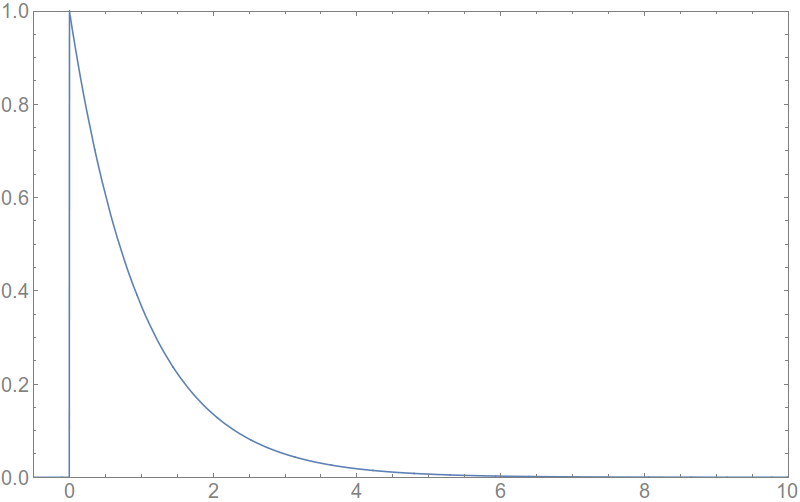
\includegraphics[width=0.4\textwidth]{pdf.png}\\
\vspace{1ex}
\onslide<3->
$F(\tau)=1-\expo{-\boldsymbol{a}\tau}$\\
\vspace{1ex}
\begin{overprint}
 \onslide<4->
\begin{center}
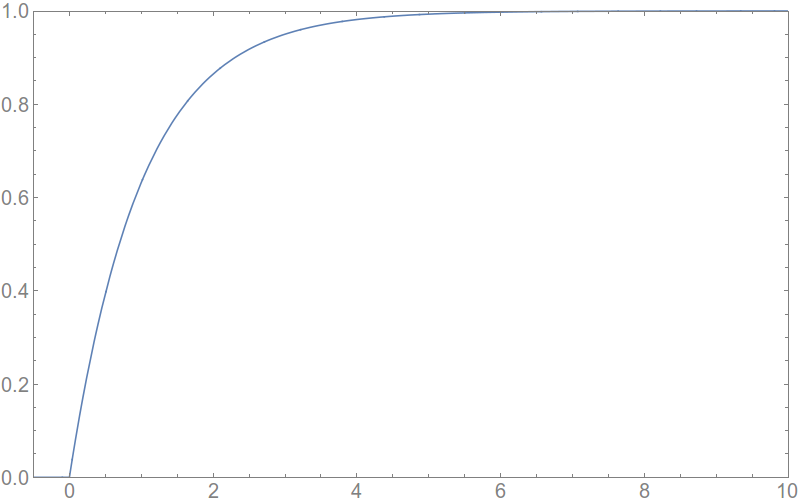
\includegraphics[width=0.40\textwidth]{cdf.png} 
\end{center}
% \\
\onslide<5->
\begin{center}
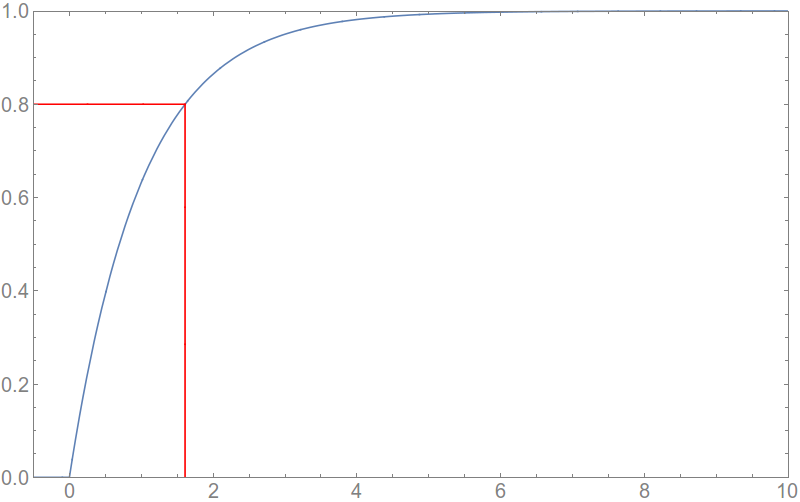
\includegraphics[width=0.40\textwidth]{cumul.png} 
\end{center}
% \\
\end{overprint}


\end{frame}

\begin{frame}
\frametitle{Drawing from $P_t(\tau,\mu)$ - The Monte Carlo Step}
\onslide<1->
 \begin{block}{Answer for $P(\tau)$}
  \onslide<2-> Generate a random number $r=rand()$ \\
\onslide<3-> Solve $r=F(\tau)$\\
\onslide<4-> So $\tau=-\frac{1}{a}\log (1-r)$
 \end{block}

\onslide<5->
\begin{block}{Answer for $P(\mu|\tau)=\frac{a_\mu}{\boldsymbol a}$}
 \onslide<6->
Generate a random number $s=rand()$\\
\onslide<7->
Invert $s=F(\mu|\tau)=\sum_{\nu=1}^\mu\frac{a_\nu}{\boldsymbol a}$\\
\onslide<8->
Find $\mu$ such that \\
\onslide<9->
$\sum_{\nu=1}^{\mu-1}\frac{a_\nu}{\boldsymbol a} < s \leq \sum_{\nu=1}^{\mu}\frac{a_\nu}{\boldsymbol a} $
\end{block}


\end{frame}





\section{Simulating Stochastic Networks}
\begin{frame}
\frametitle{What's the Story for Networks}

\centering
\adjustbox{max height=\dimexpr\textheight-5.5cm\relax,
           max width=\textwidth}{
\onslide<1->
\begin{tabular}{crcc}
&   &     
    \begin{minipage}{.3\textwidth}
\centering
      \uncover<3->{
\includegraphics[width=0.65\linewidth]{Ill.png}}
    \end{minipage} &
 \begin{minipage}{.3\textwidth}
\centering
      \uncover<5->{
\includegraphics[width=.7\linewidth]{infandsusc.png}}
    \end{minipage}
\\
% \multicolumn{1}{r}{
  \begin{minipage}{.5\textwidth}
\begin{tabular}{c}
      \uncover<1->{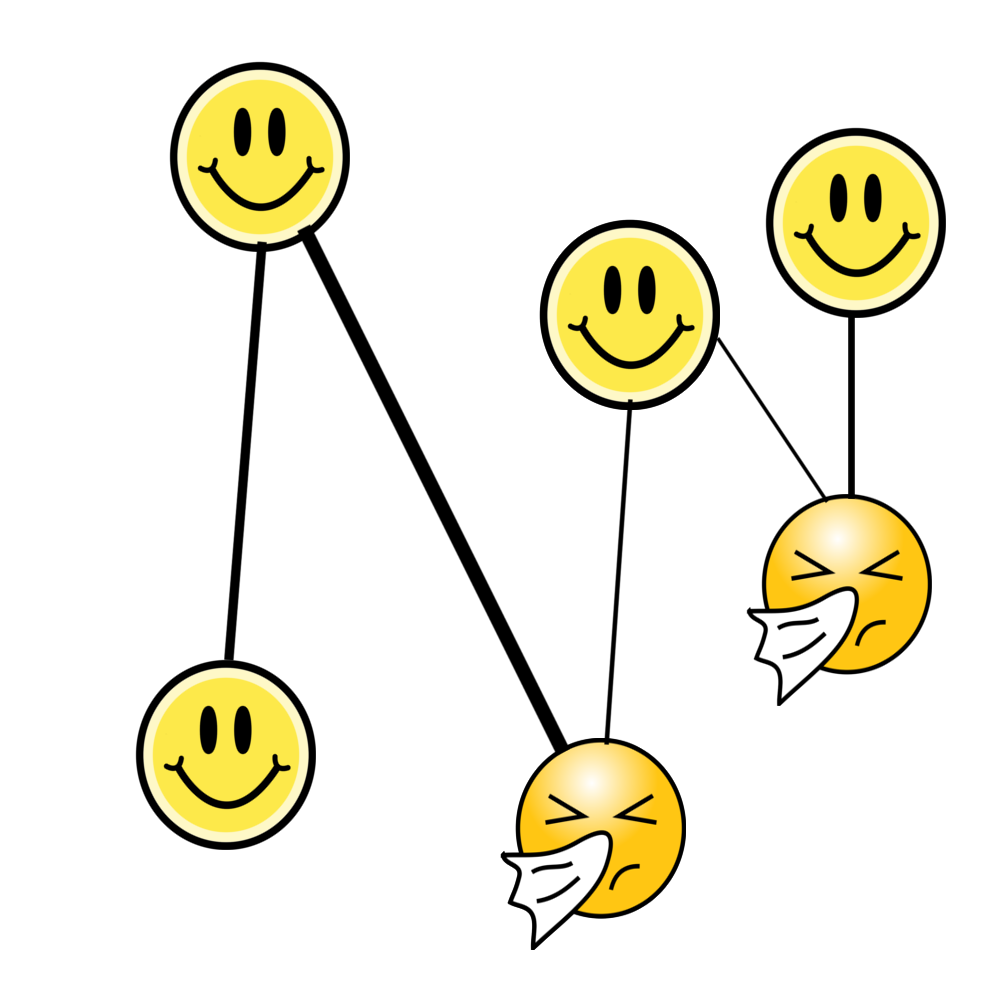
\includegraphics[width=\linewidth]{network.png}}\\
\uncover<1->{$\boldsymbol{x}=(x_i)\,,\,\boldsymbol{A}=(A_{ij})$}
\end{tabular}
    \end{minipage}
&
\uncover<2->{\textbf{Reaction :}}  & 
\begin{minipage}{.3\textwidth}
\centering
\uncover<4->{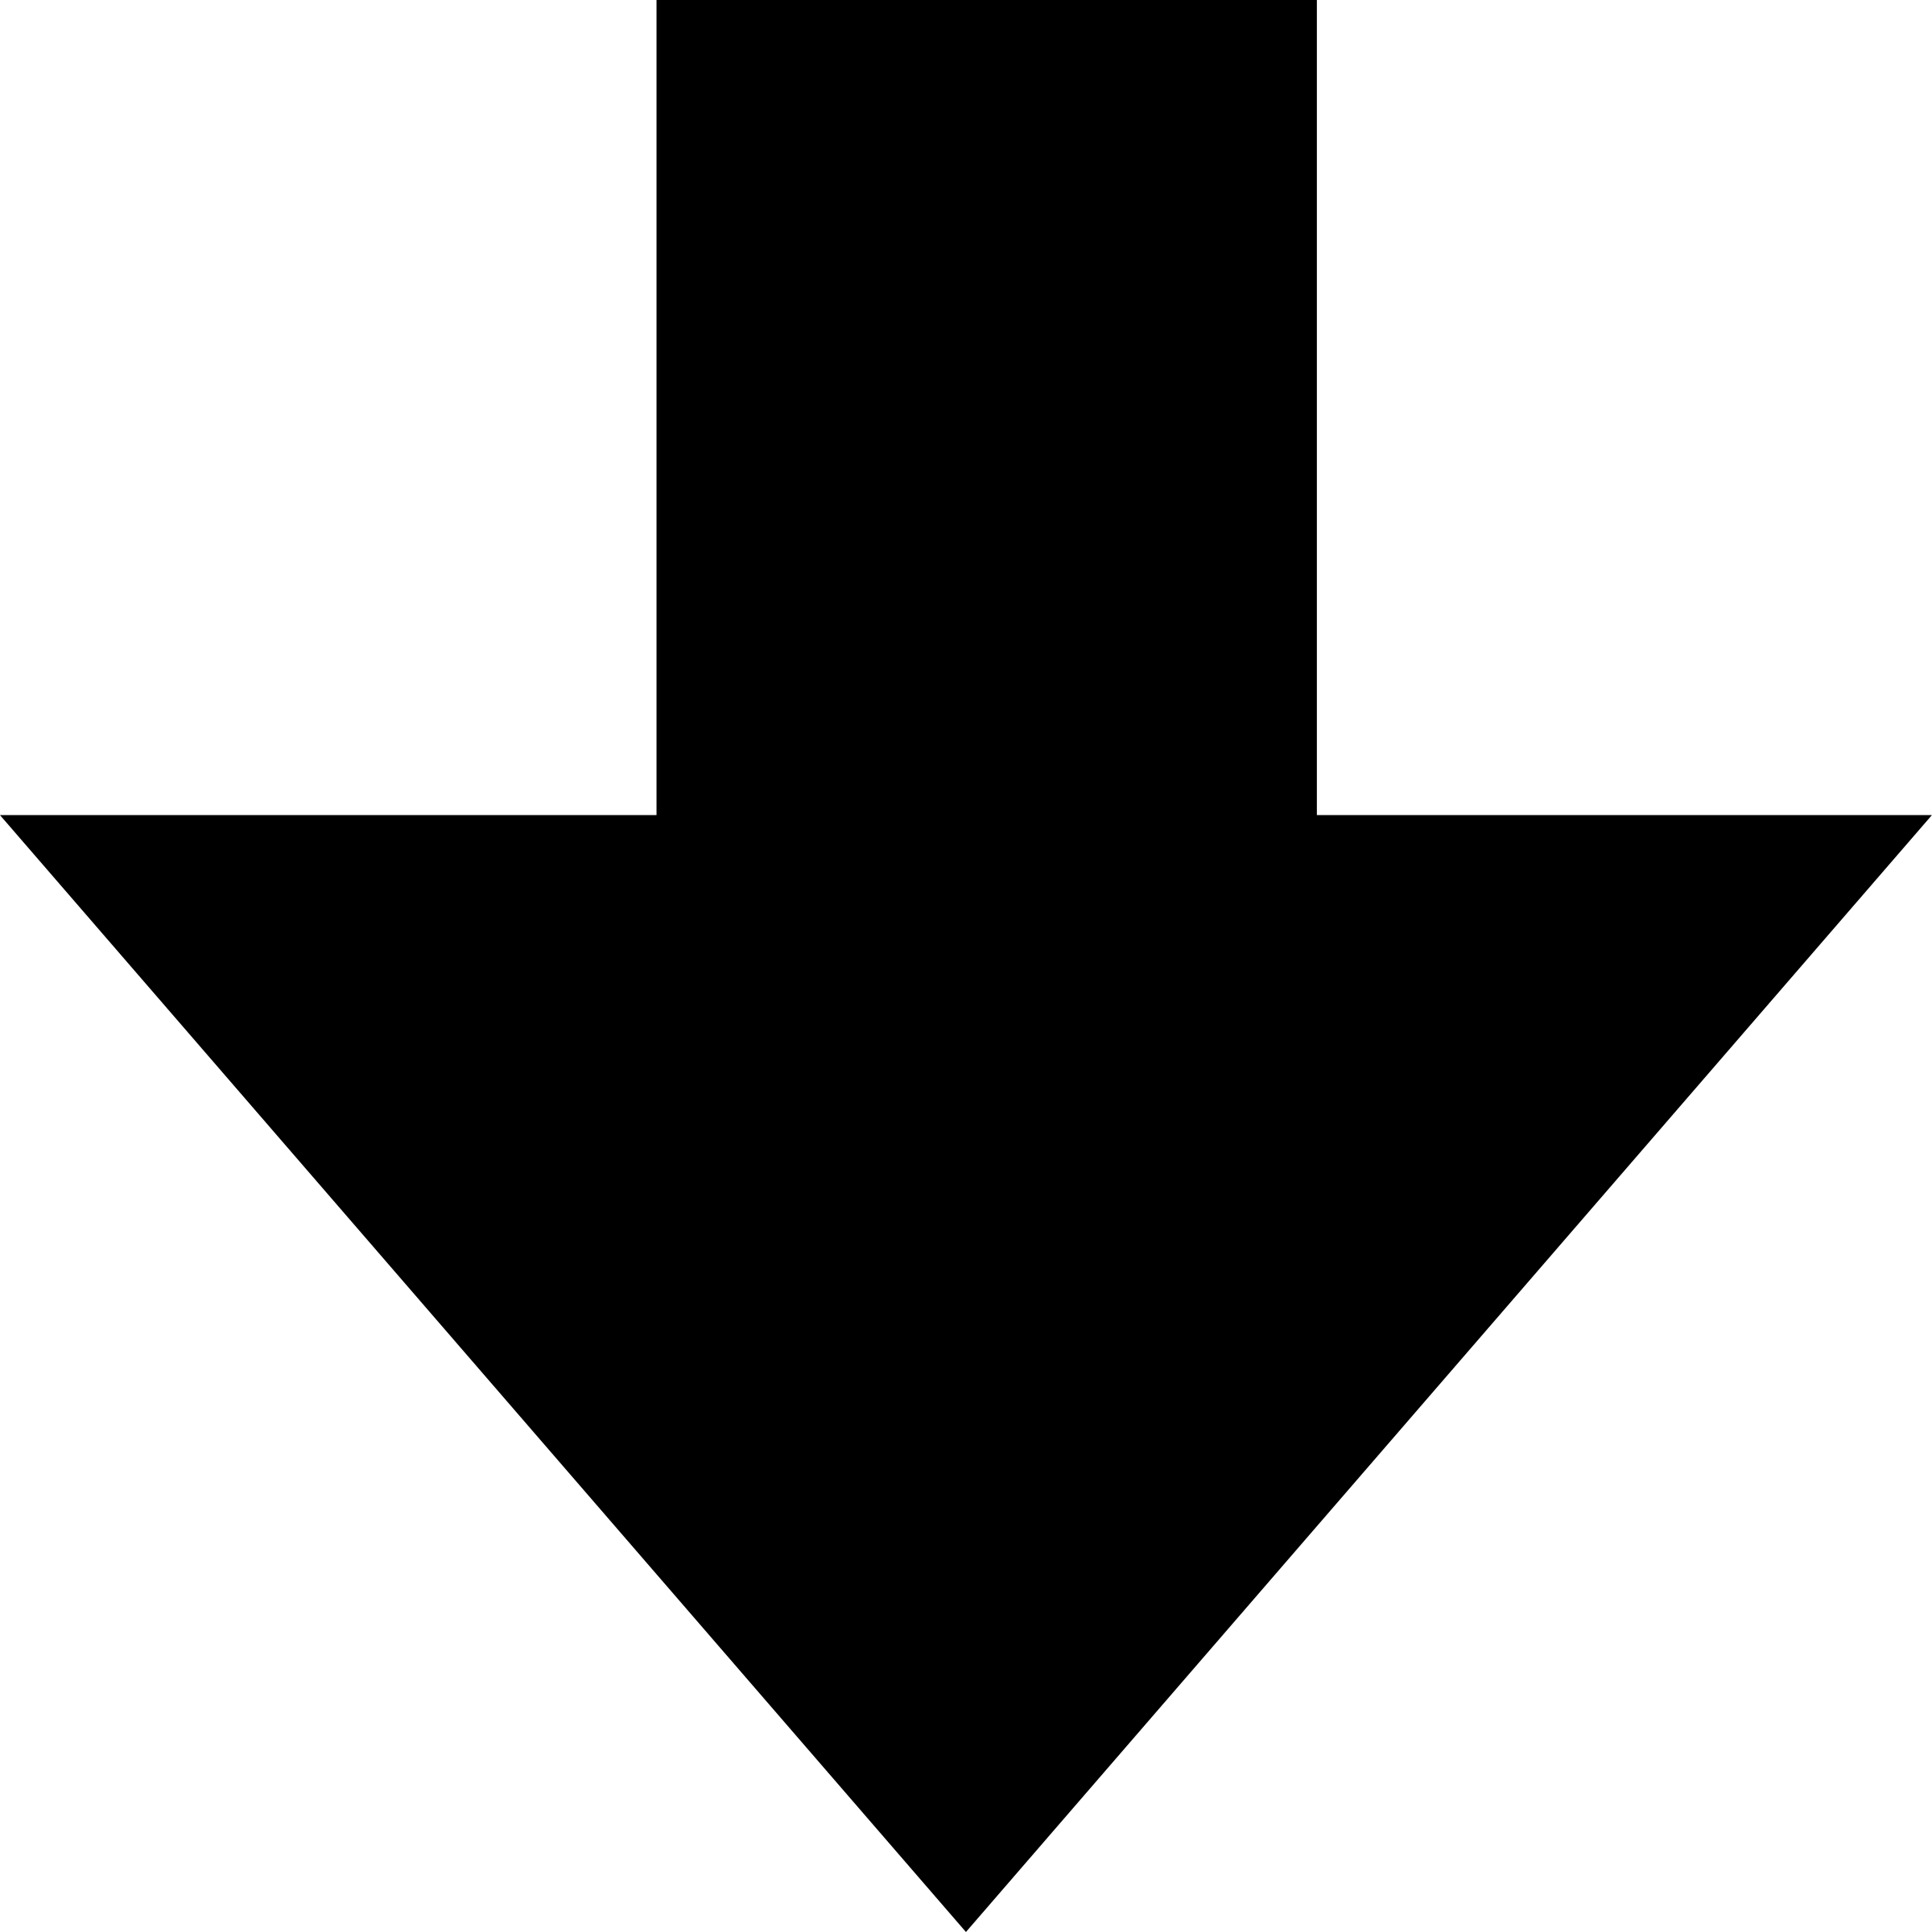
\includegraphics[width=0.2\linewidth]{downarrow.png}}
% \end{center}
    \end{minipage} 
  &     \begin{minipage}{.3\textwidth}
%       \begin{center}
\centering
\uncover<6->{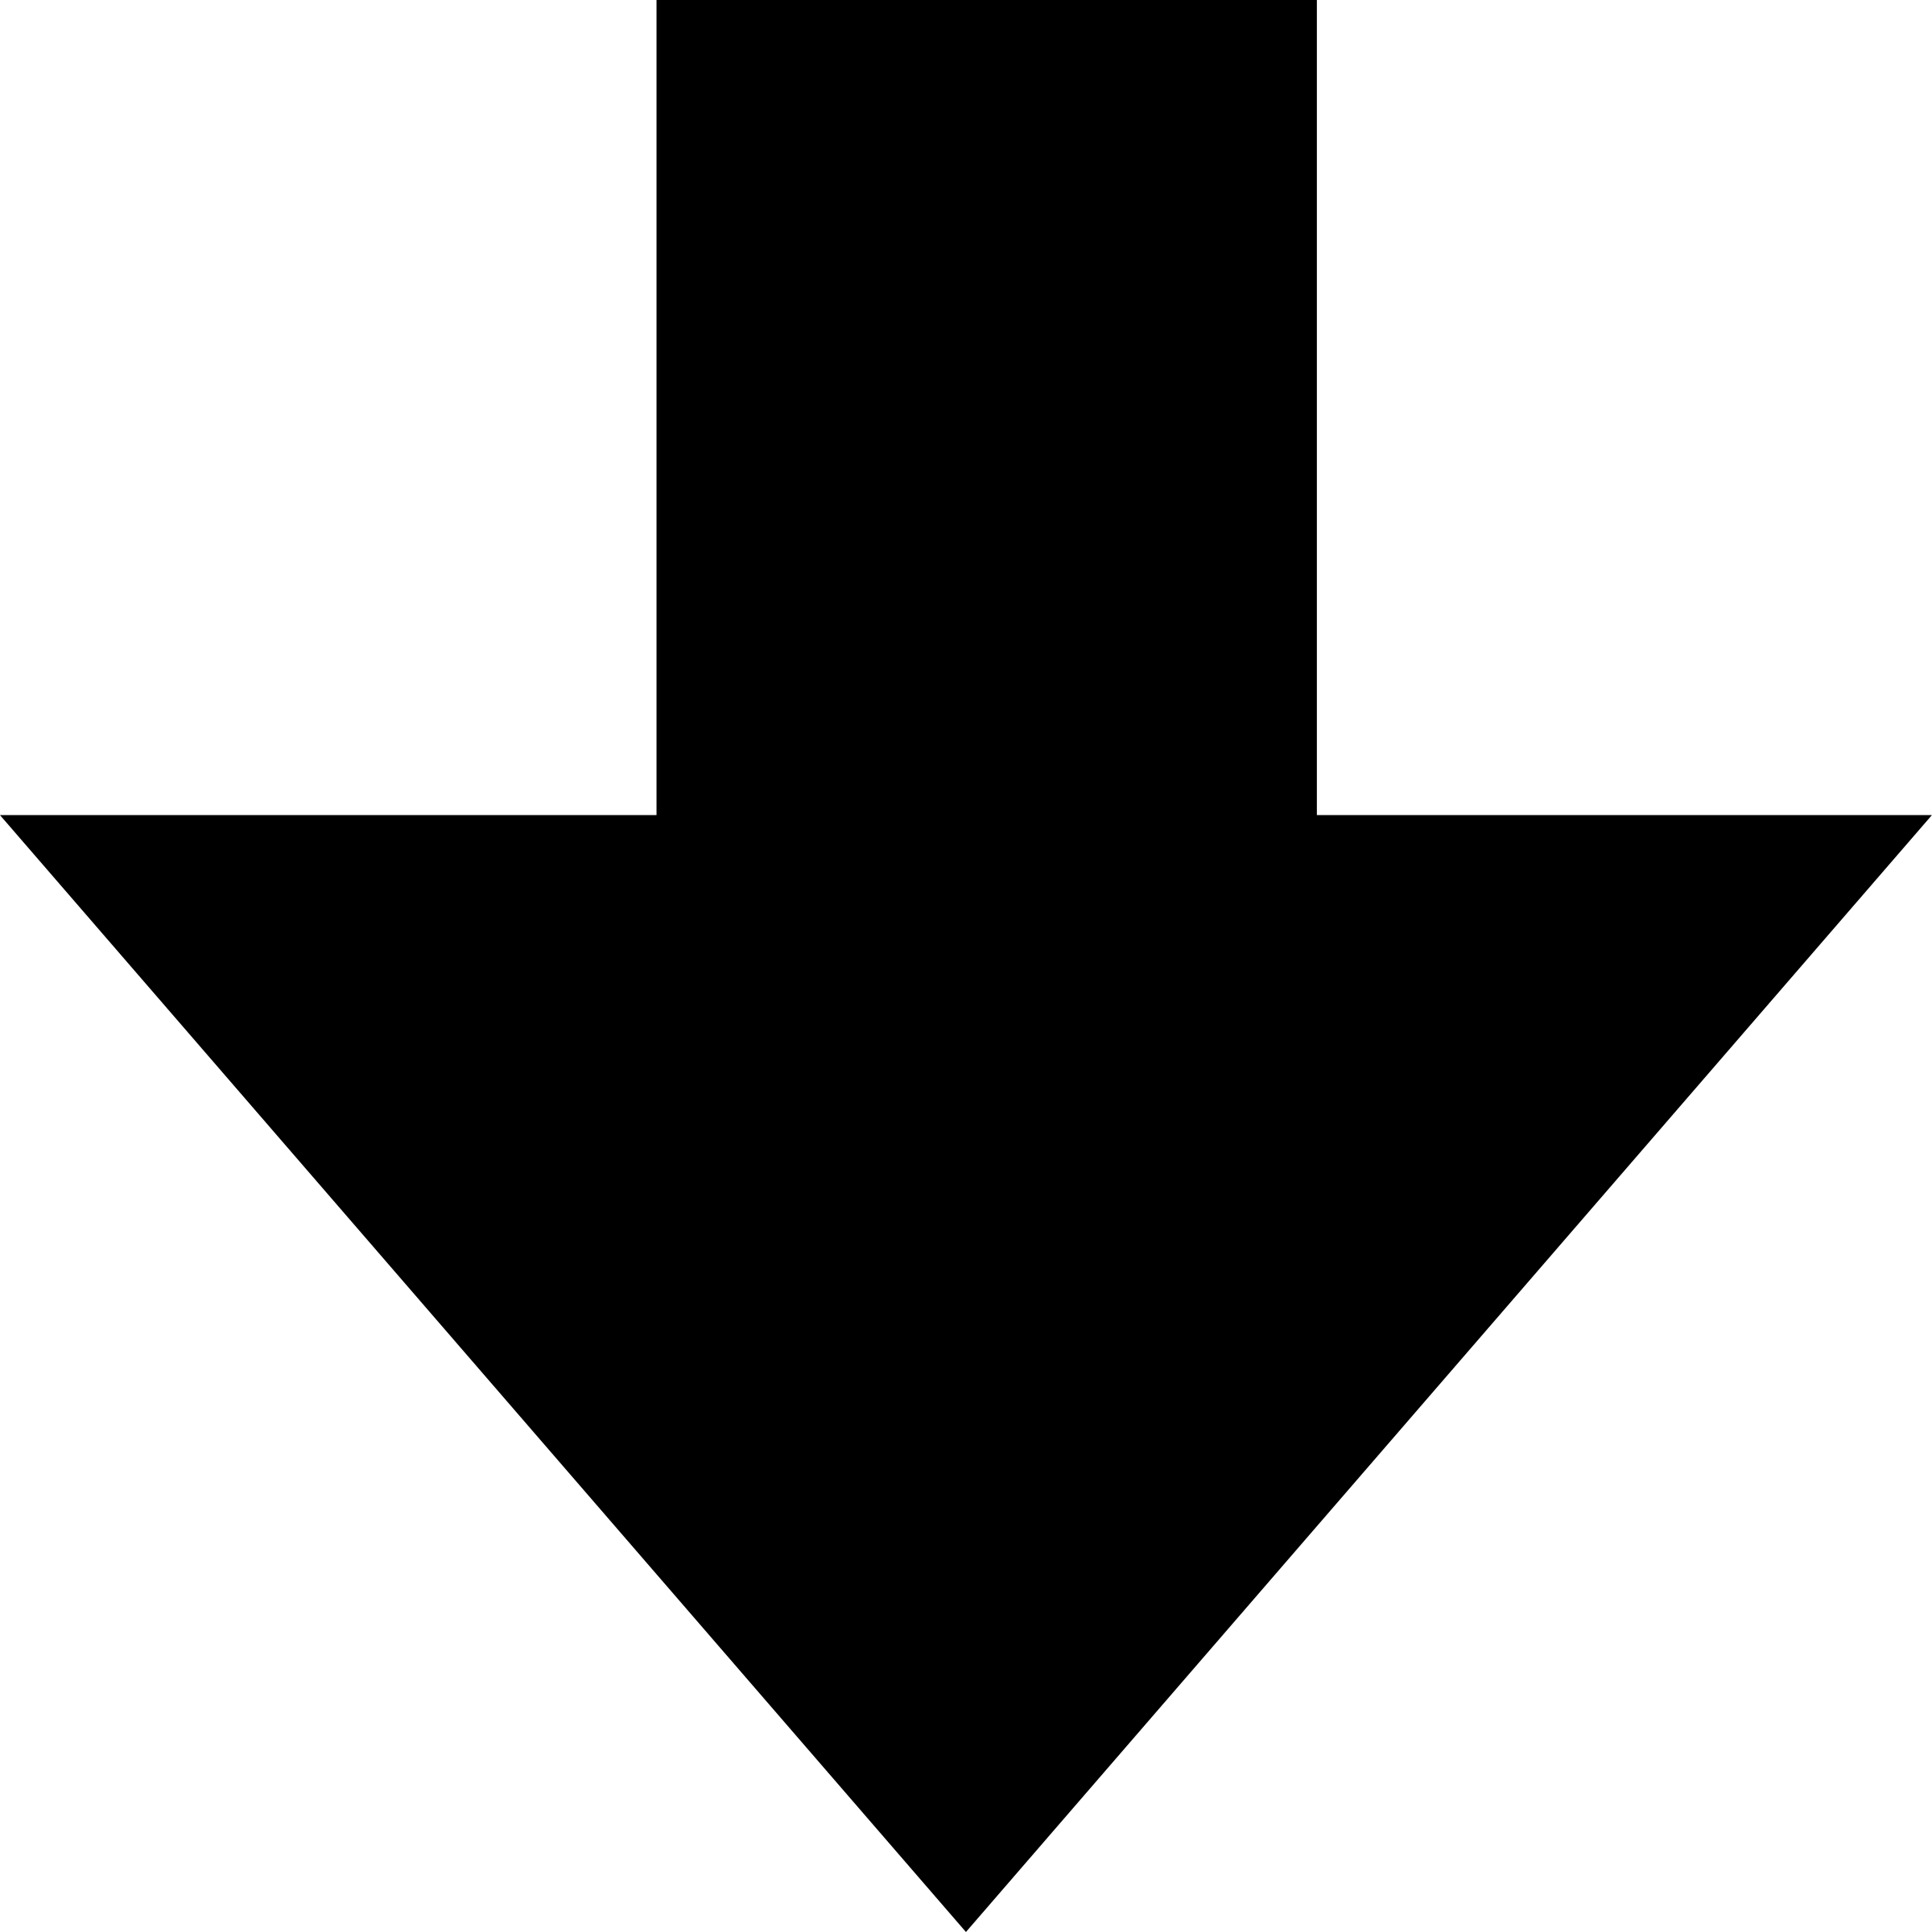
\includegraphics[width=0.2\linewidth]{downarrow.png}}
% \end{center}
    \end{minipage} 
 \\
 & &
    \begin{minipage}{.3\textwidth}
\centering
      \onslide<4->
\includegraphics[width=0.65\linewidth]{Smiley.png}
    \end{minipage} &  \begin{minipage}{.3\textwidth}
\centering
      \uncover<6->{
\includegraphics[width=0.7\linewidth]{bothill.png}}
    \end{minipage} 
\\
\rule{0pt}{4ex}  
 & \onslide<7-> \textbf{Number of Reactants:} & $h_1$ \onslide<8->$=N_I$\uncover<9>{$=\sum_ix_i$}  & \onslide<11->$h_2$\onslide<12->$=N_{SI}$\uncover<13>{$=\sum_{ij}(1-x_i)A_{ij}x_j$}\\
\rule{0pt}{4ex}  
 & \onslide<15-> \textbf{Reaction Rates:} & $r$  & $\lambda \qquad\qquad$%& $c_3$& $\dots$ & $c_M$
\end{tabular}
}

\end{frame}

\begin{frame}
 \frametitle{Implementation - Initialisation}
% \adjustbox{max height=\dimexpr\textheight-5.5cm\relax,
%            max width=\textwidth}{
\onslide<1->
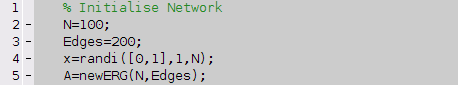
\includegraphics[width=\linewidth]{initial1.png}\\
\onslide<2->
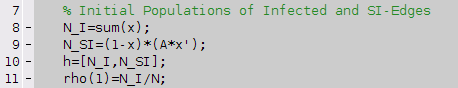
\includegraphics[width=\linewidth]{initial2.png}\\
\onslide<3->
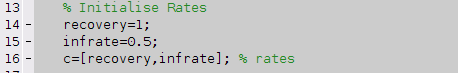
\includegraphics[width=\linewidth]{initial3.png}\\
\onslide<4->
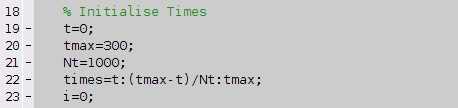
\includegraphics[width=\linewidth]{initial4.png}
\end{frame}

\begin{frame}
 \frametitle{Implementation - Iteration}
% \adjustbox{max height=\dimexpr\textheight-5.5cm\relax,
%            max width=\textwidth}{
\onslide<1->
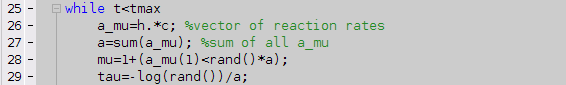
\includegraphics[width=\linewidth]{iter1.png}\\
\onslide<2->
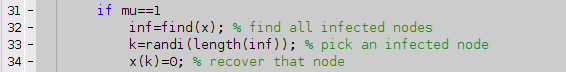
\includegraphics[width=\linewidth]{iter2.png}\\
\onslide<3->
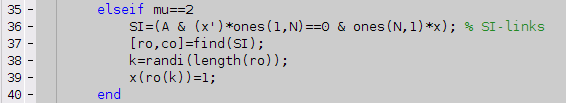
\includegraphics[width=\linewidth]{iter3.png}\\
\onslide<4->
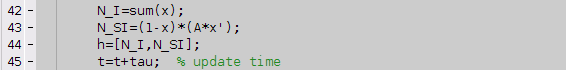
\includegraphics[width=\linewidth]{iter4.png}\\
\vspace{2ex}
\onslide<5->
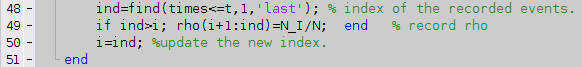
\includegraphics[width=\linewidth]{iter5.png}
\end{frame}

\begin{frame}
 \frametitle{Implementation - Sample Path I}
\onslide<1->
\centering
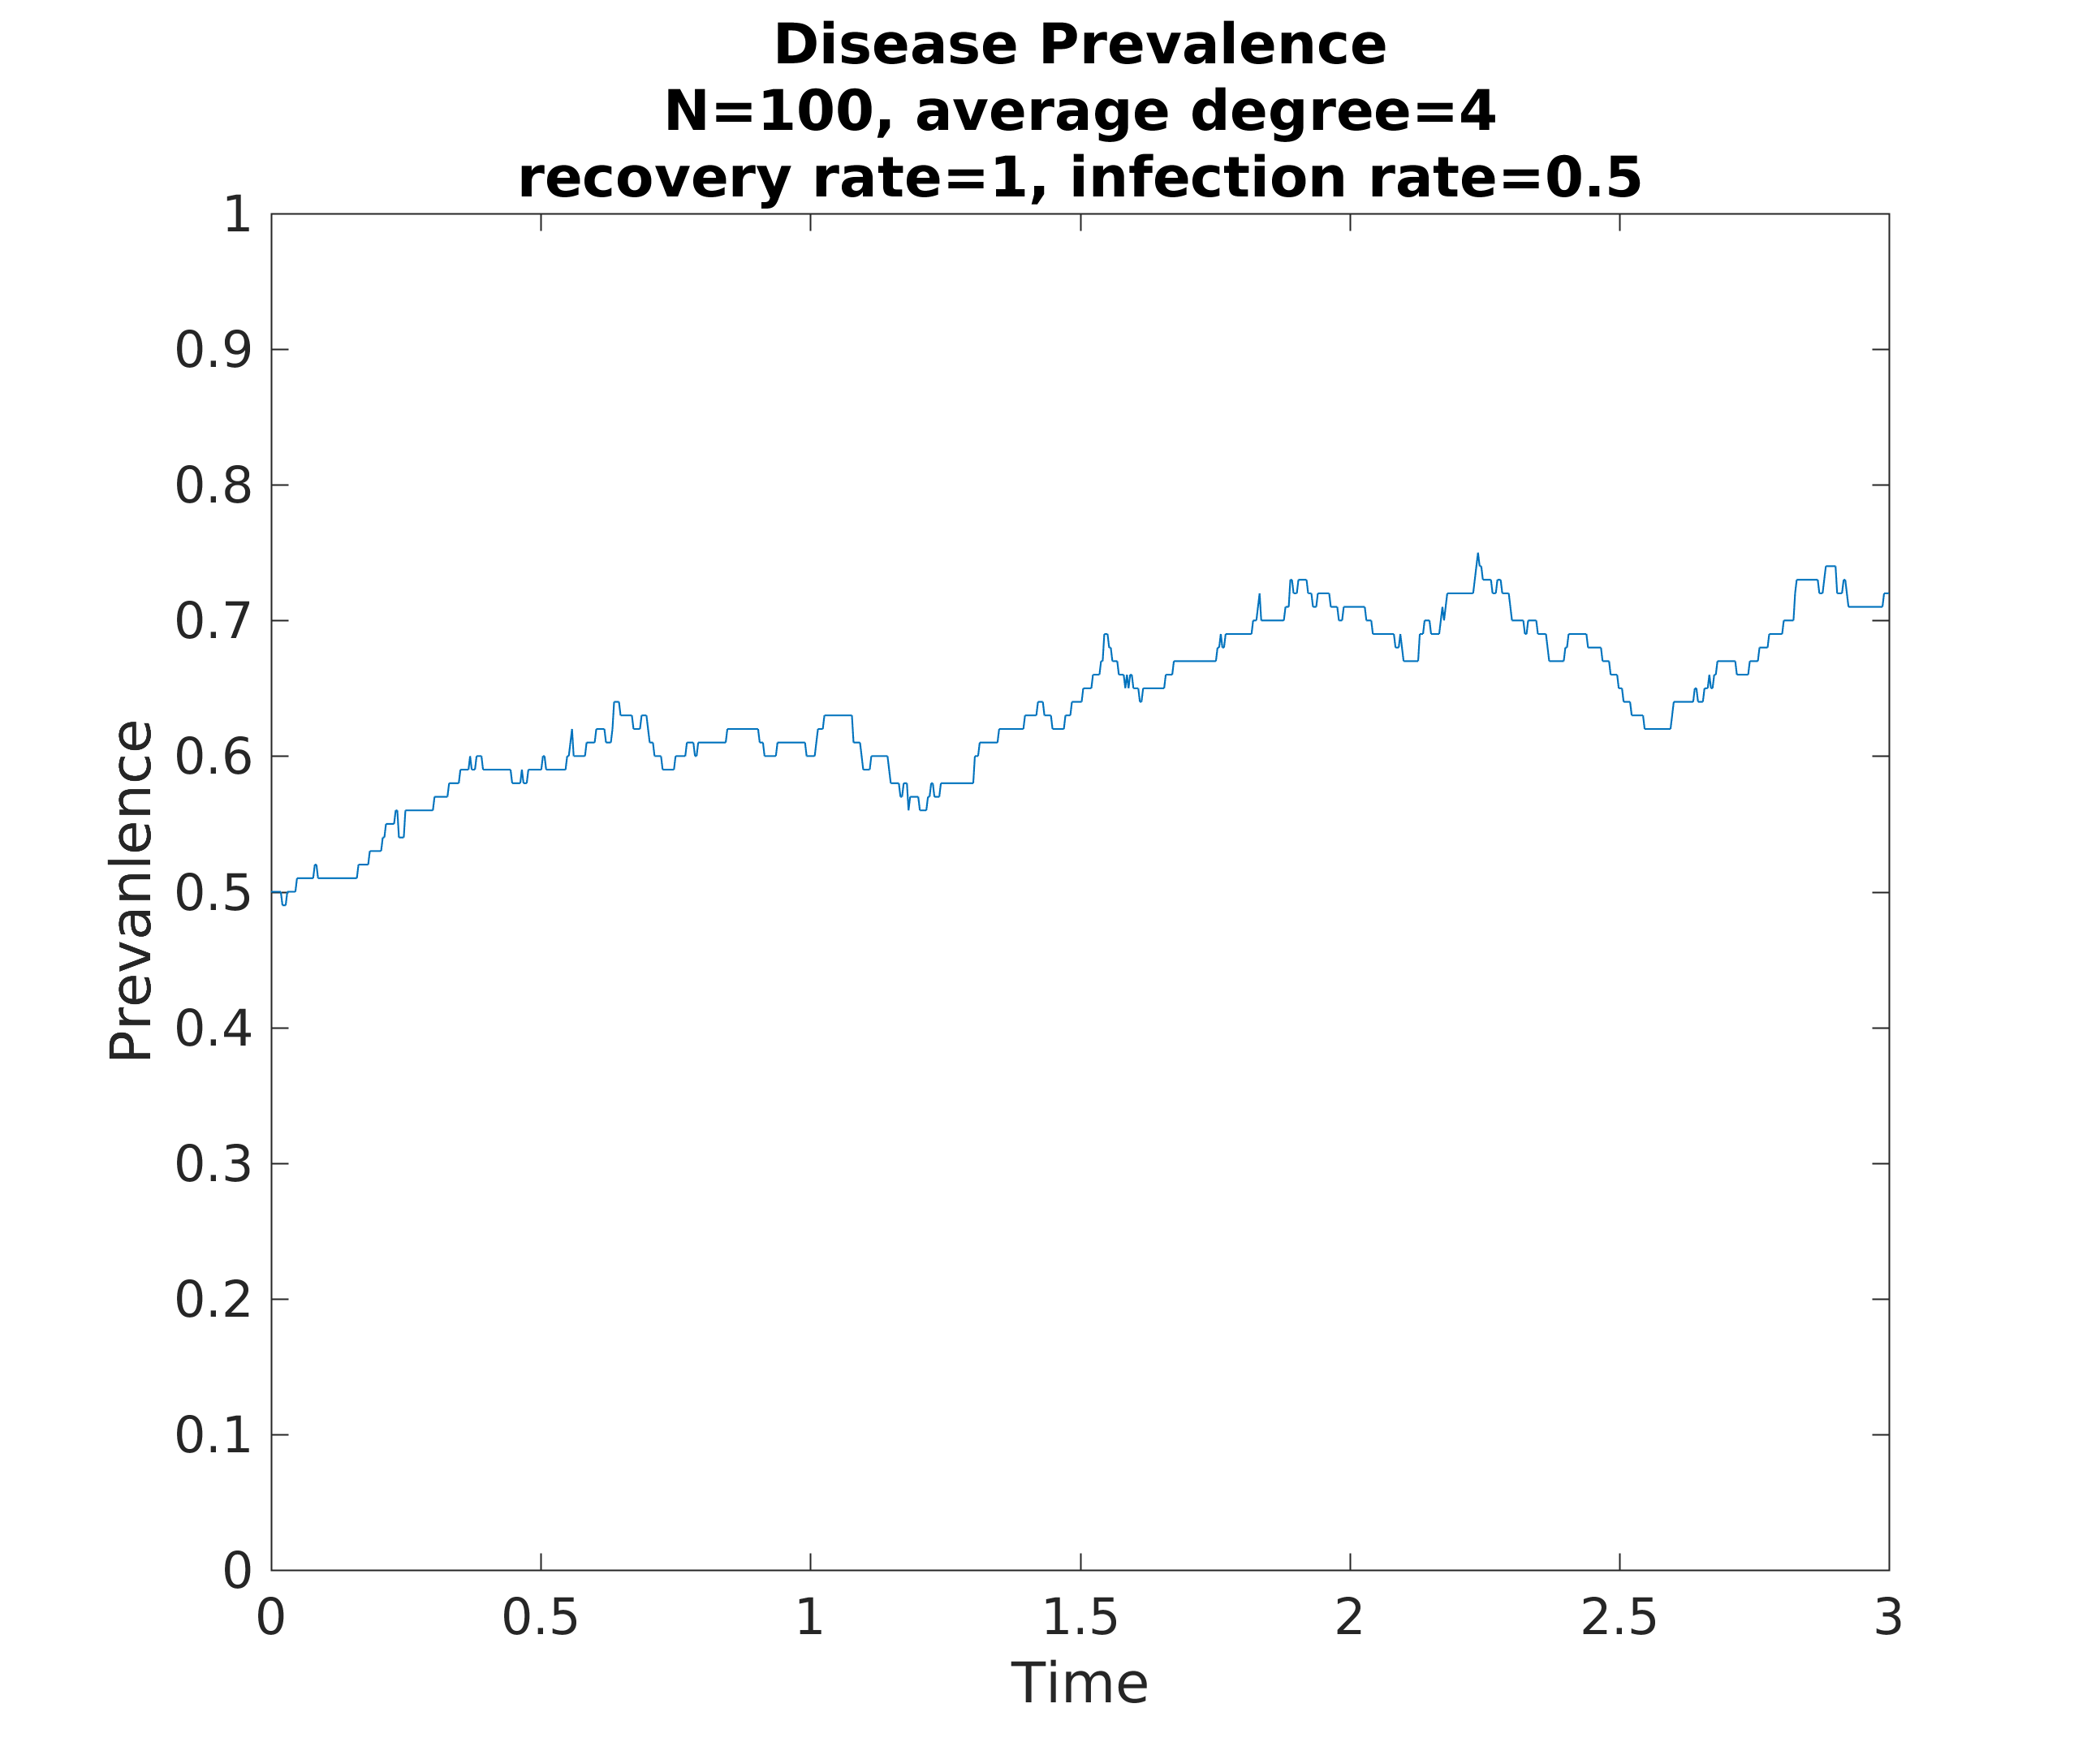
\includegraphics[width=.75\textwidth]{samplepath3secnorew.png}
\end{frame}

\begin{frame}
 \frametitle{Implementation - Sample Path II}
\onslide<1->
\centering
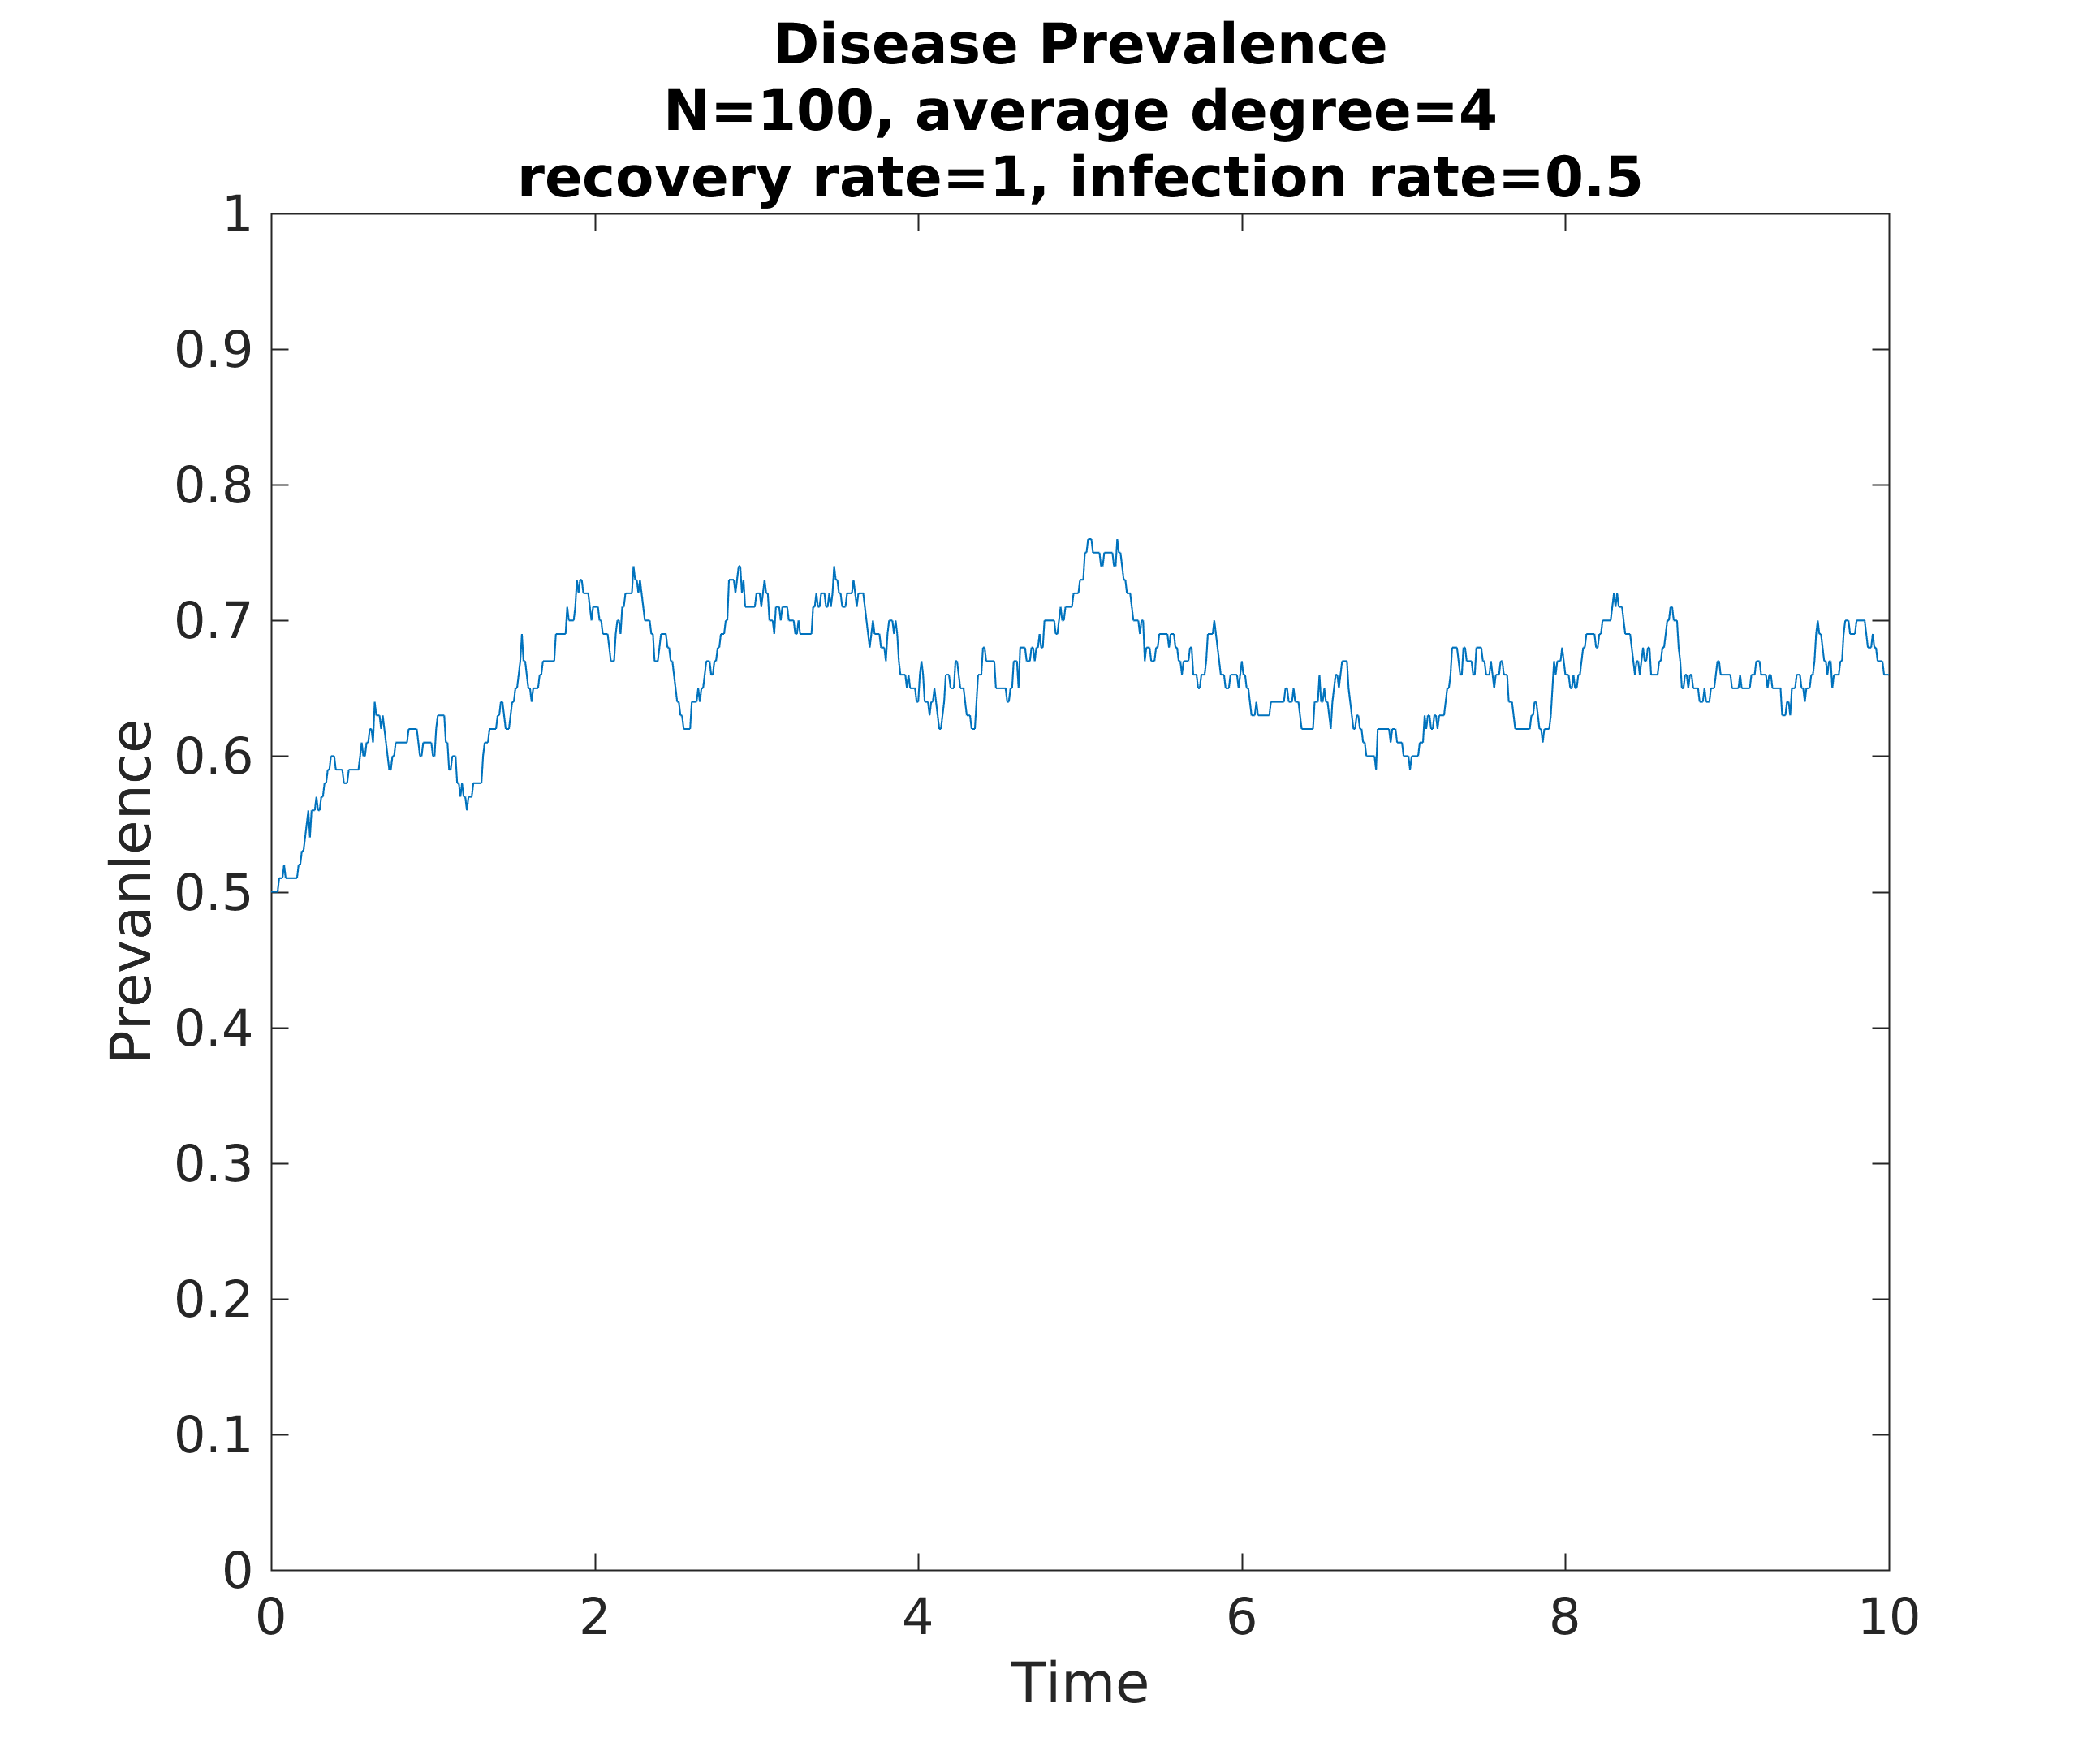
\includegraphics[width=.75\textwidth]{samplepath10secnorew.png}
\end{frame}

\begin{frame}
 \frametitle{But How about Adaptive Networks?}
\centering
\adjustbox{max height=\dimexpr\textheight-5.5cm\relax,
           max width=\textwidth}{
\onslide<1->
\begin{tabular}{rccc}
&    
    \begin{minipage}{.3\textwidth}
\centering
      \uncover<1->{
\includegraphics[width=0.65\linewidth]{Ill.png}}
    \end{minipage} &
 \begin{minipage}{.3\textwidth}
\centering
      \uncover<1->{
\includegraphics[width=.7\linewidth]{infandsusc.png}}
    \end{minipage} &
 \begin{minipage}{.3\textwidth}
\centering
      \uncover<2->{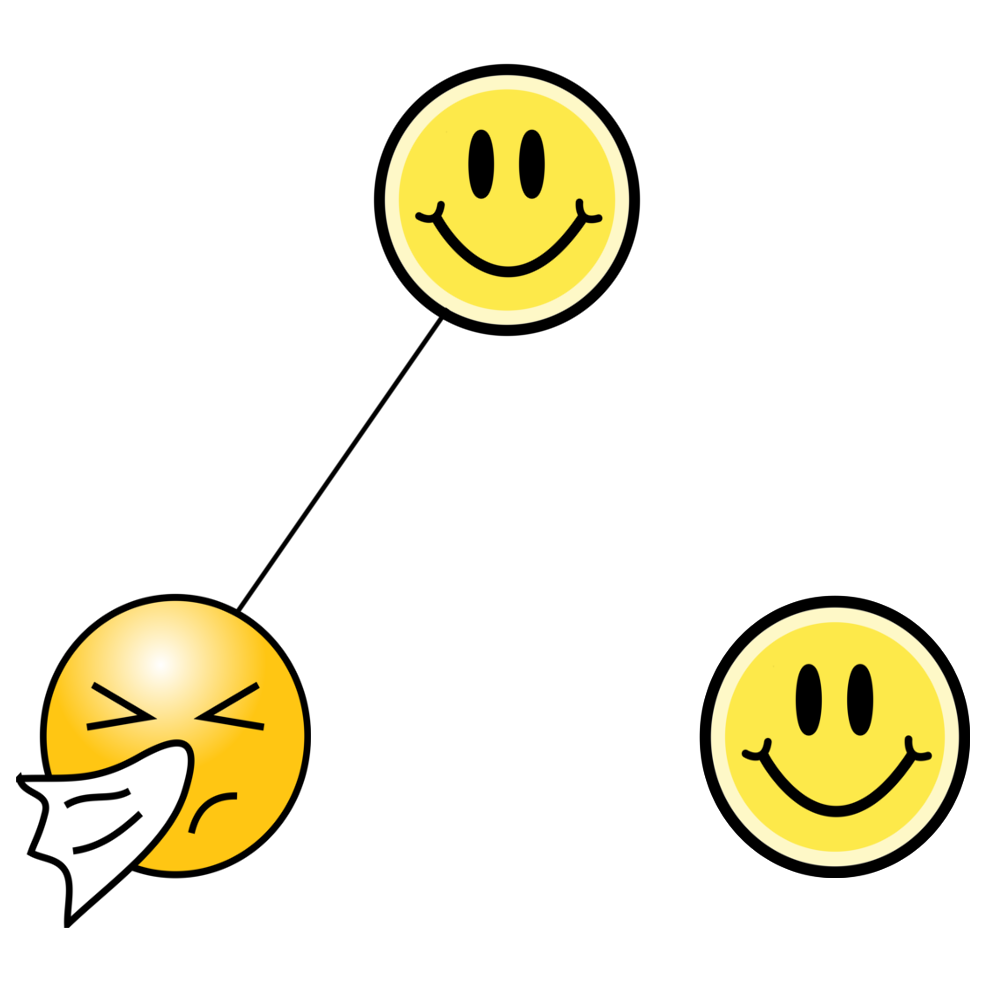
\includegraphics[width=\linewidth]{relinking1.png}}
    \end{minipage}
\\
\uncover<1->{\textbf{Reaction :}}  & 
\begin{minipage}{.3\textwidth}
\centering
\uncover<1->{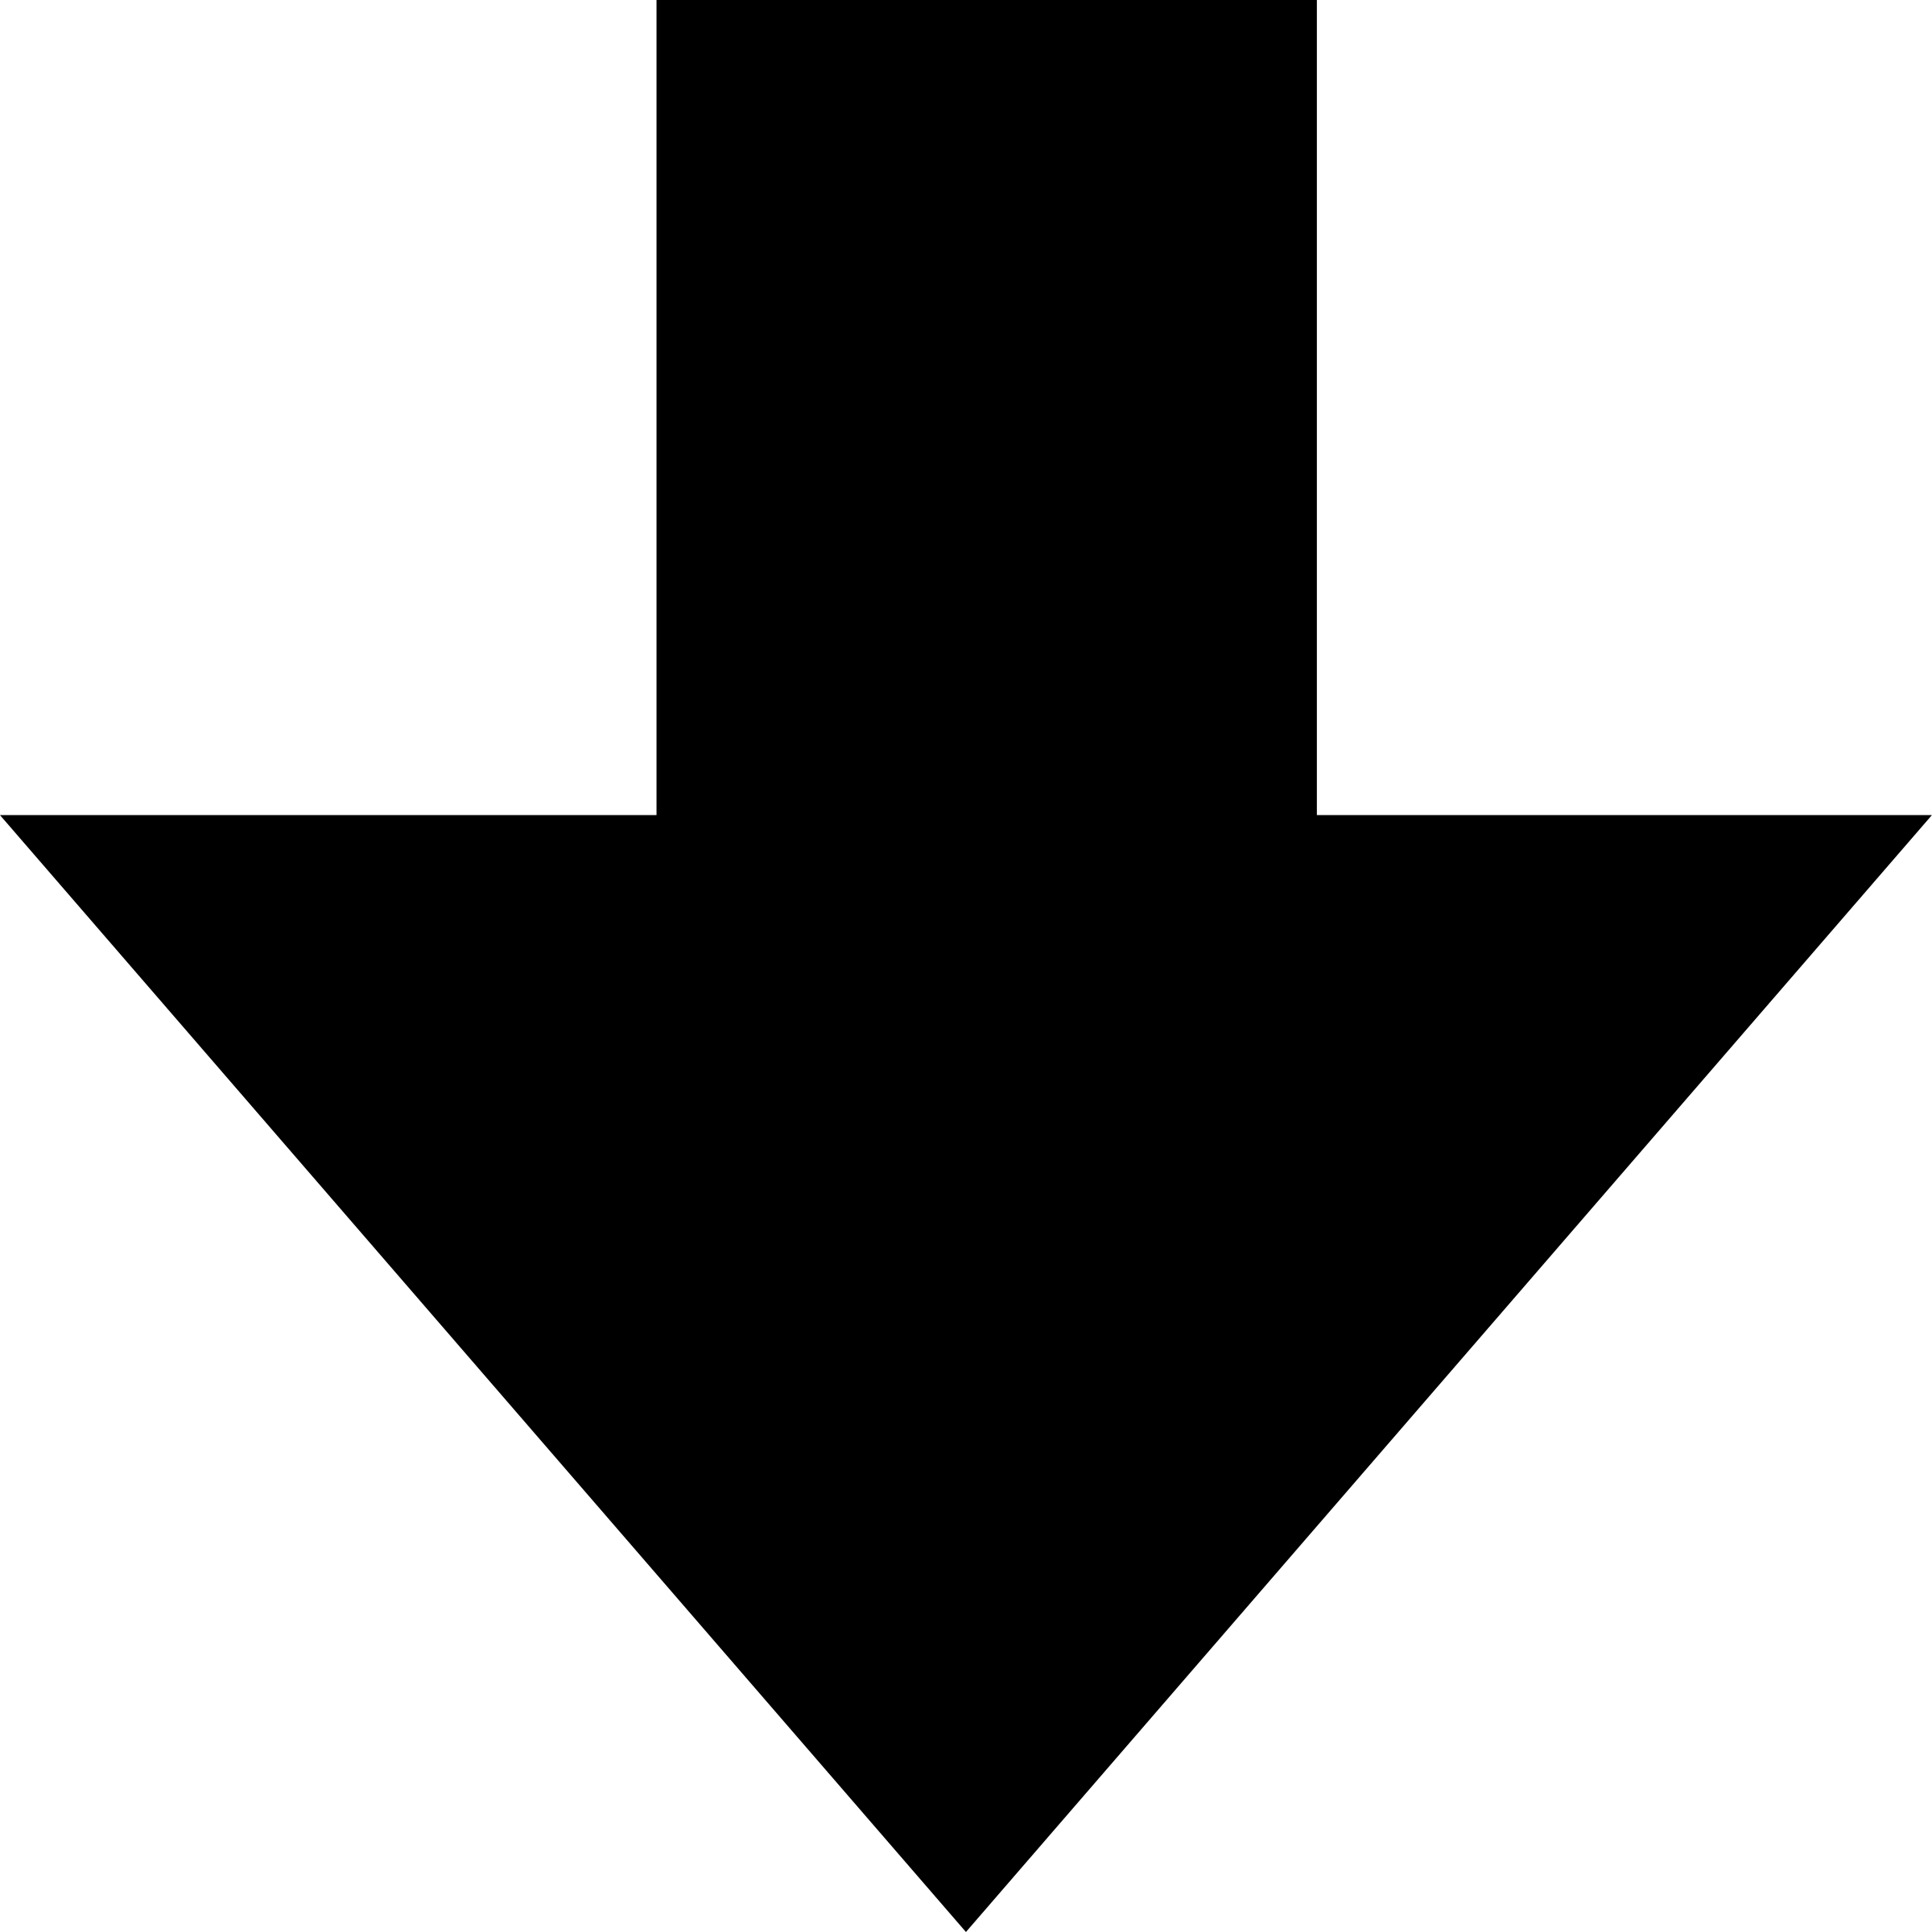
\includegraphics[width=0.2\linewidth]{downarrow.png}}
% \end{center}
    \end{minipage} 
  &     
\begin{minipage}{.3\textwidth}
%       \begin{center}
\centering
\uncover<1->{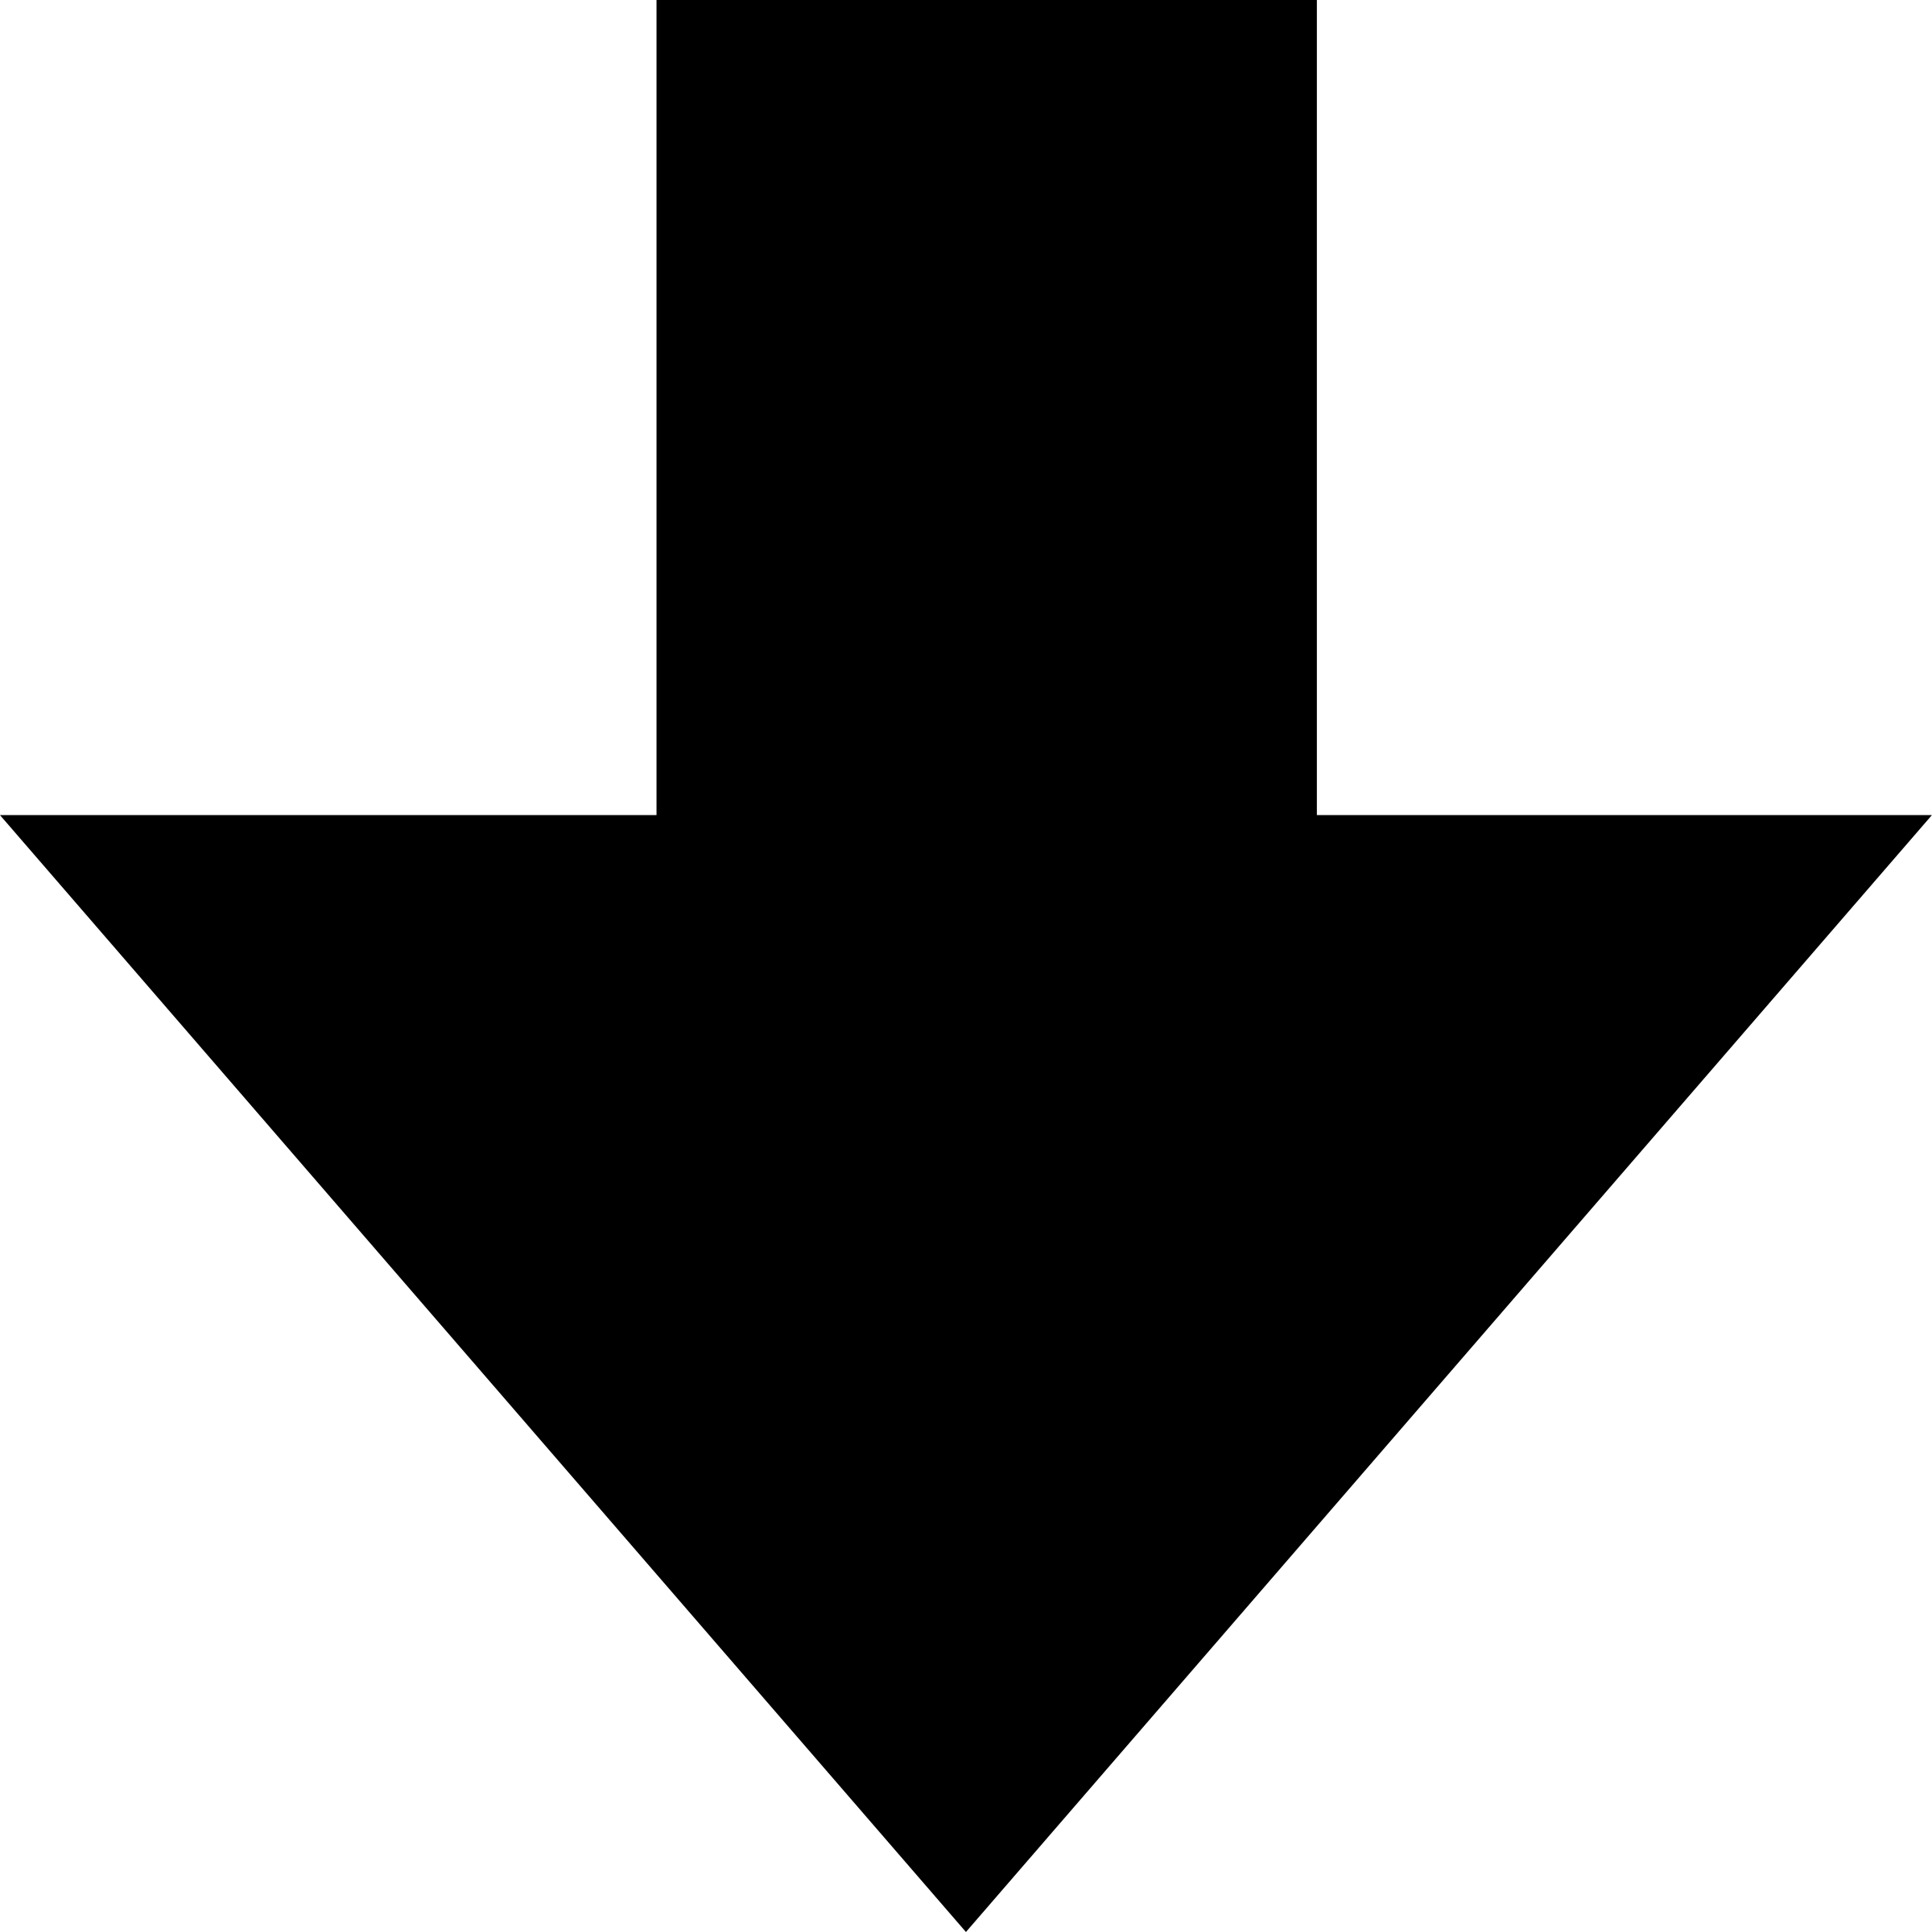
\includegraphics[width=0.2\linewidth]{downarrow.png}}
% \end{center}
    \end{minipage} 
&
\begin{minipage}{.3\textwidth}
%       \begin{center}
\centering
\uncover<3->{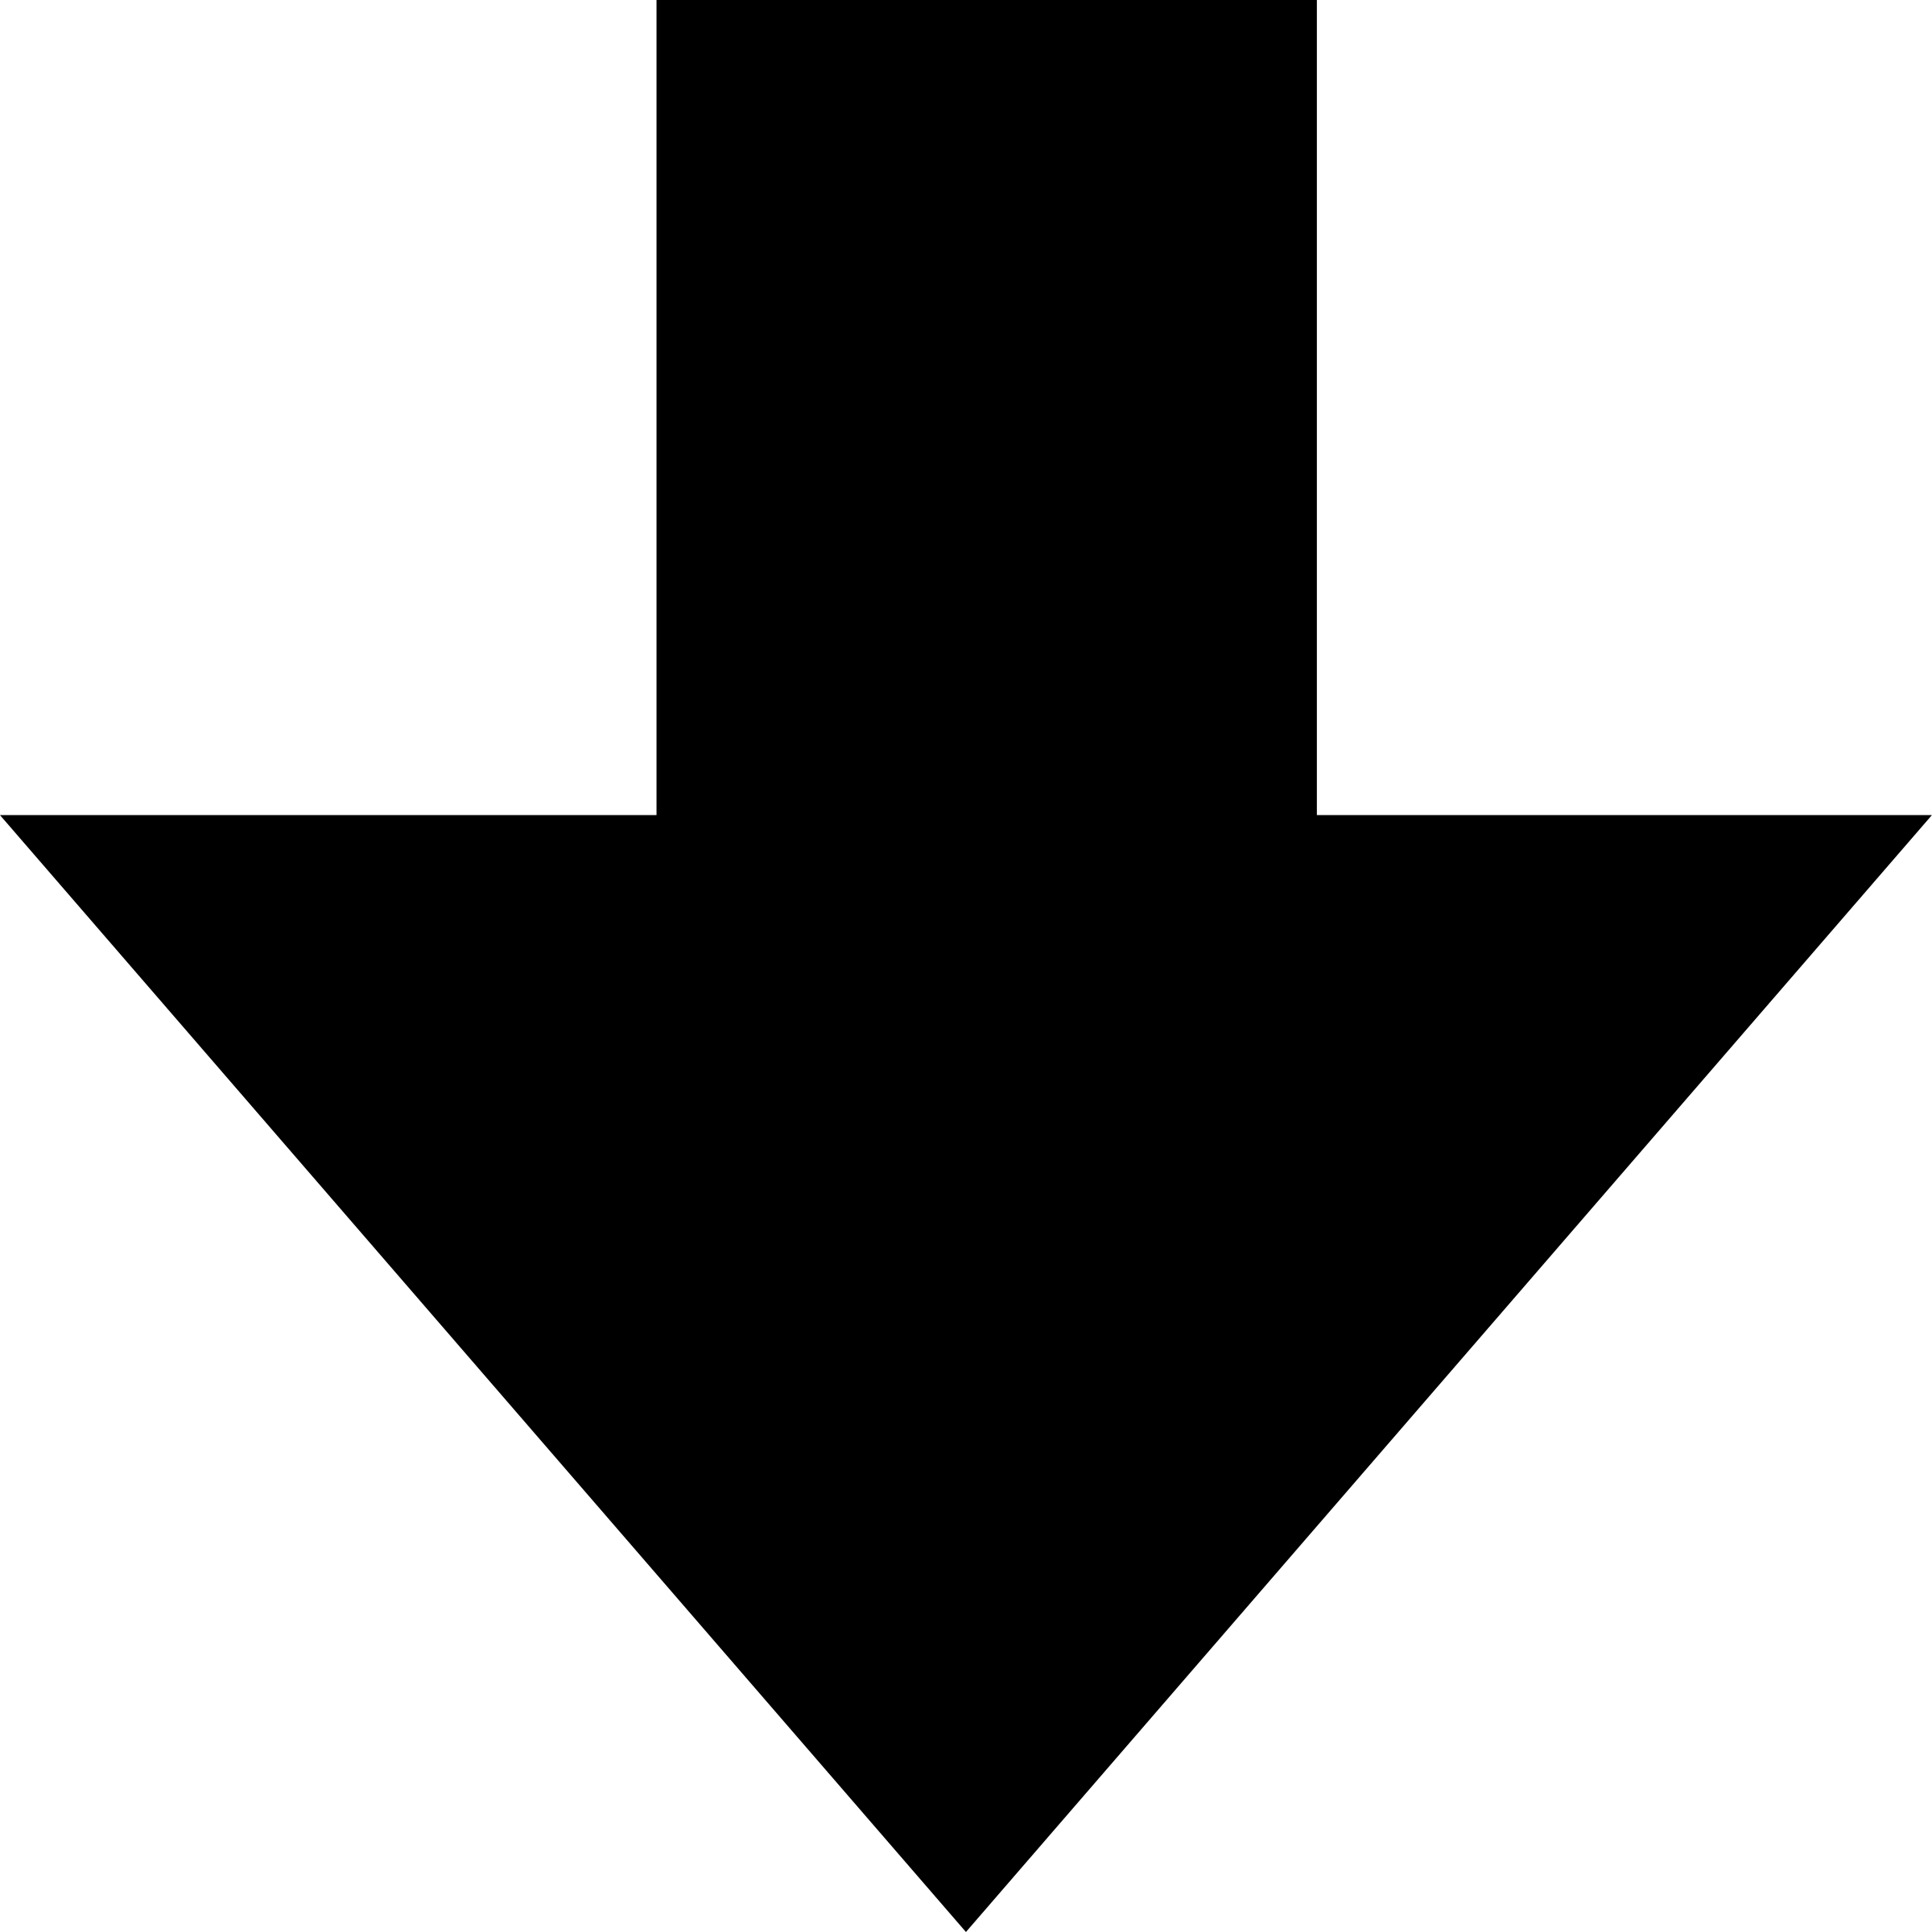
\includegraphics[width=0.2\linewidth]{downarrow.png}}
% \end{center}
    \end{minipage} 
 \\
 &
    \begin{minipage}{.3\textwidth}
\centering
      \onslide<1->
\includegraphics[width=0.65\linewidth]{Smiley.png}
    \end{minipage} &  \begin{minipage}{.3\textwidth}
\centering
      \uncover<1->{
\includegraphics[width=0.7\linewidth]{bothill.png}}
    \end{minipage} &  \begin{minipage}{.3\textwidth}
\centering
      \uncover<3->{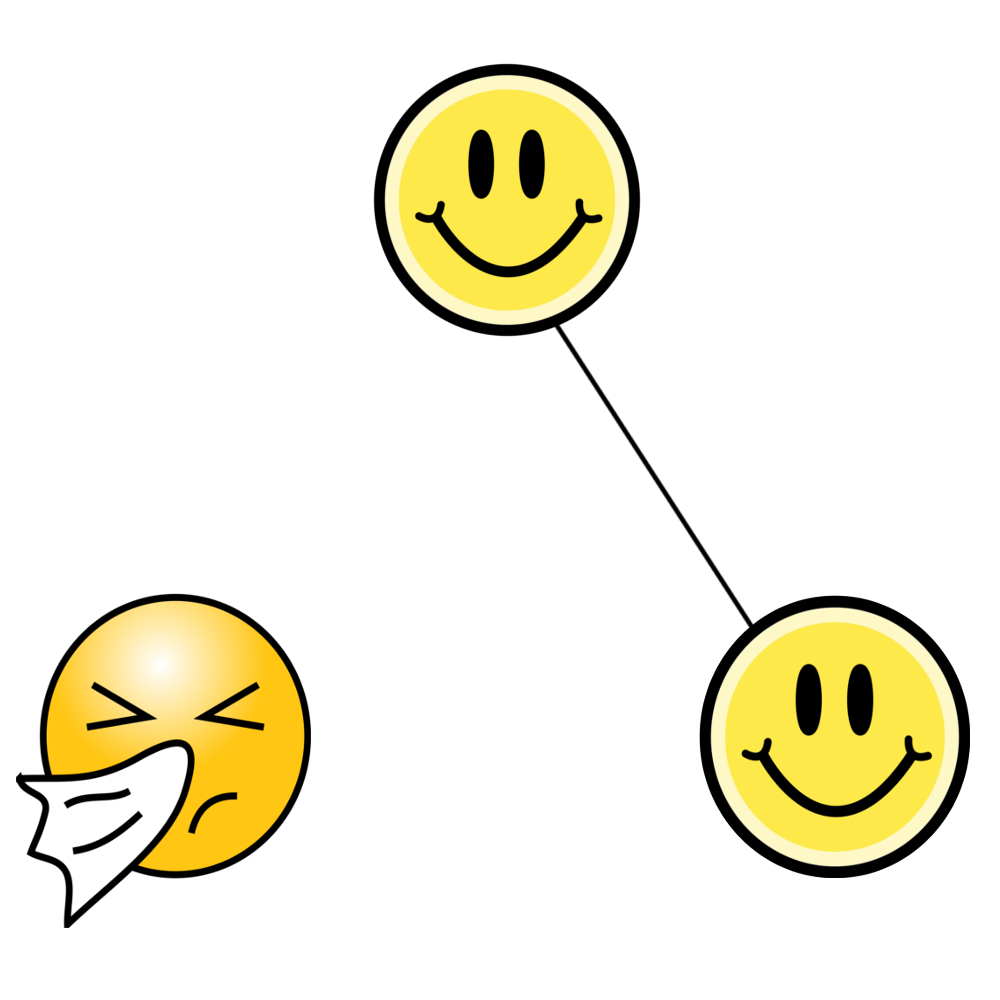
\includegraphics[width=\linewidth]{relinking2.png}}
    \end{minipage} 
\\
% \hrule{2pt}{4ex}  
\onslide<4-> \textbf{Number of Reactants:} & $h_1=N_I$ & $h_2=N_{SI}$& $h_3=N_{SI}$\onslide<5->${}^{\!\!\!\!\!\!*}$\\
\rule{0pt}{4ex}  
\onslide<6-> \textbf{Reaction Rates:} & $r$  & $\lambda$  & \onslide<7-> $w$ %& $c_3$& $\dots$ & $c_M$
\end{tabular}
}
\end{frame}


\begin{frame}
 \frametitle{Implementation - Sample Path II}
\onslide<1->
\centering
\adjustbox{max height=\dimexpr\textheight-5.5cm\relax,
           max width=\textwidth}{
\onslide<1->
\begin{tabular}{rccc}
\begin{minipage}{\linewidth}
\centering
 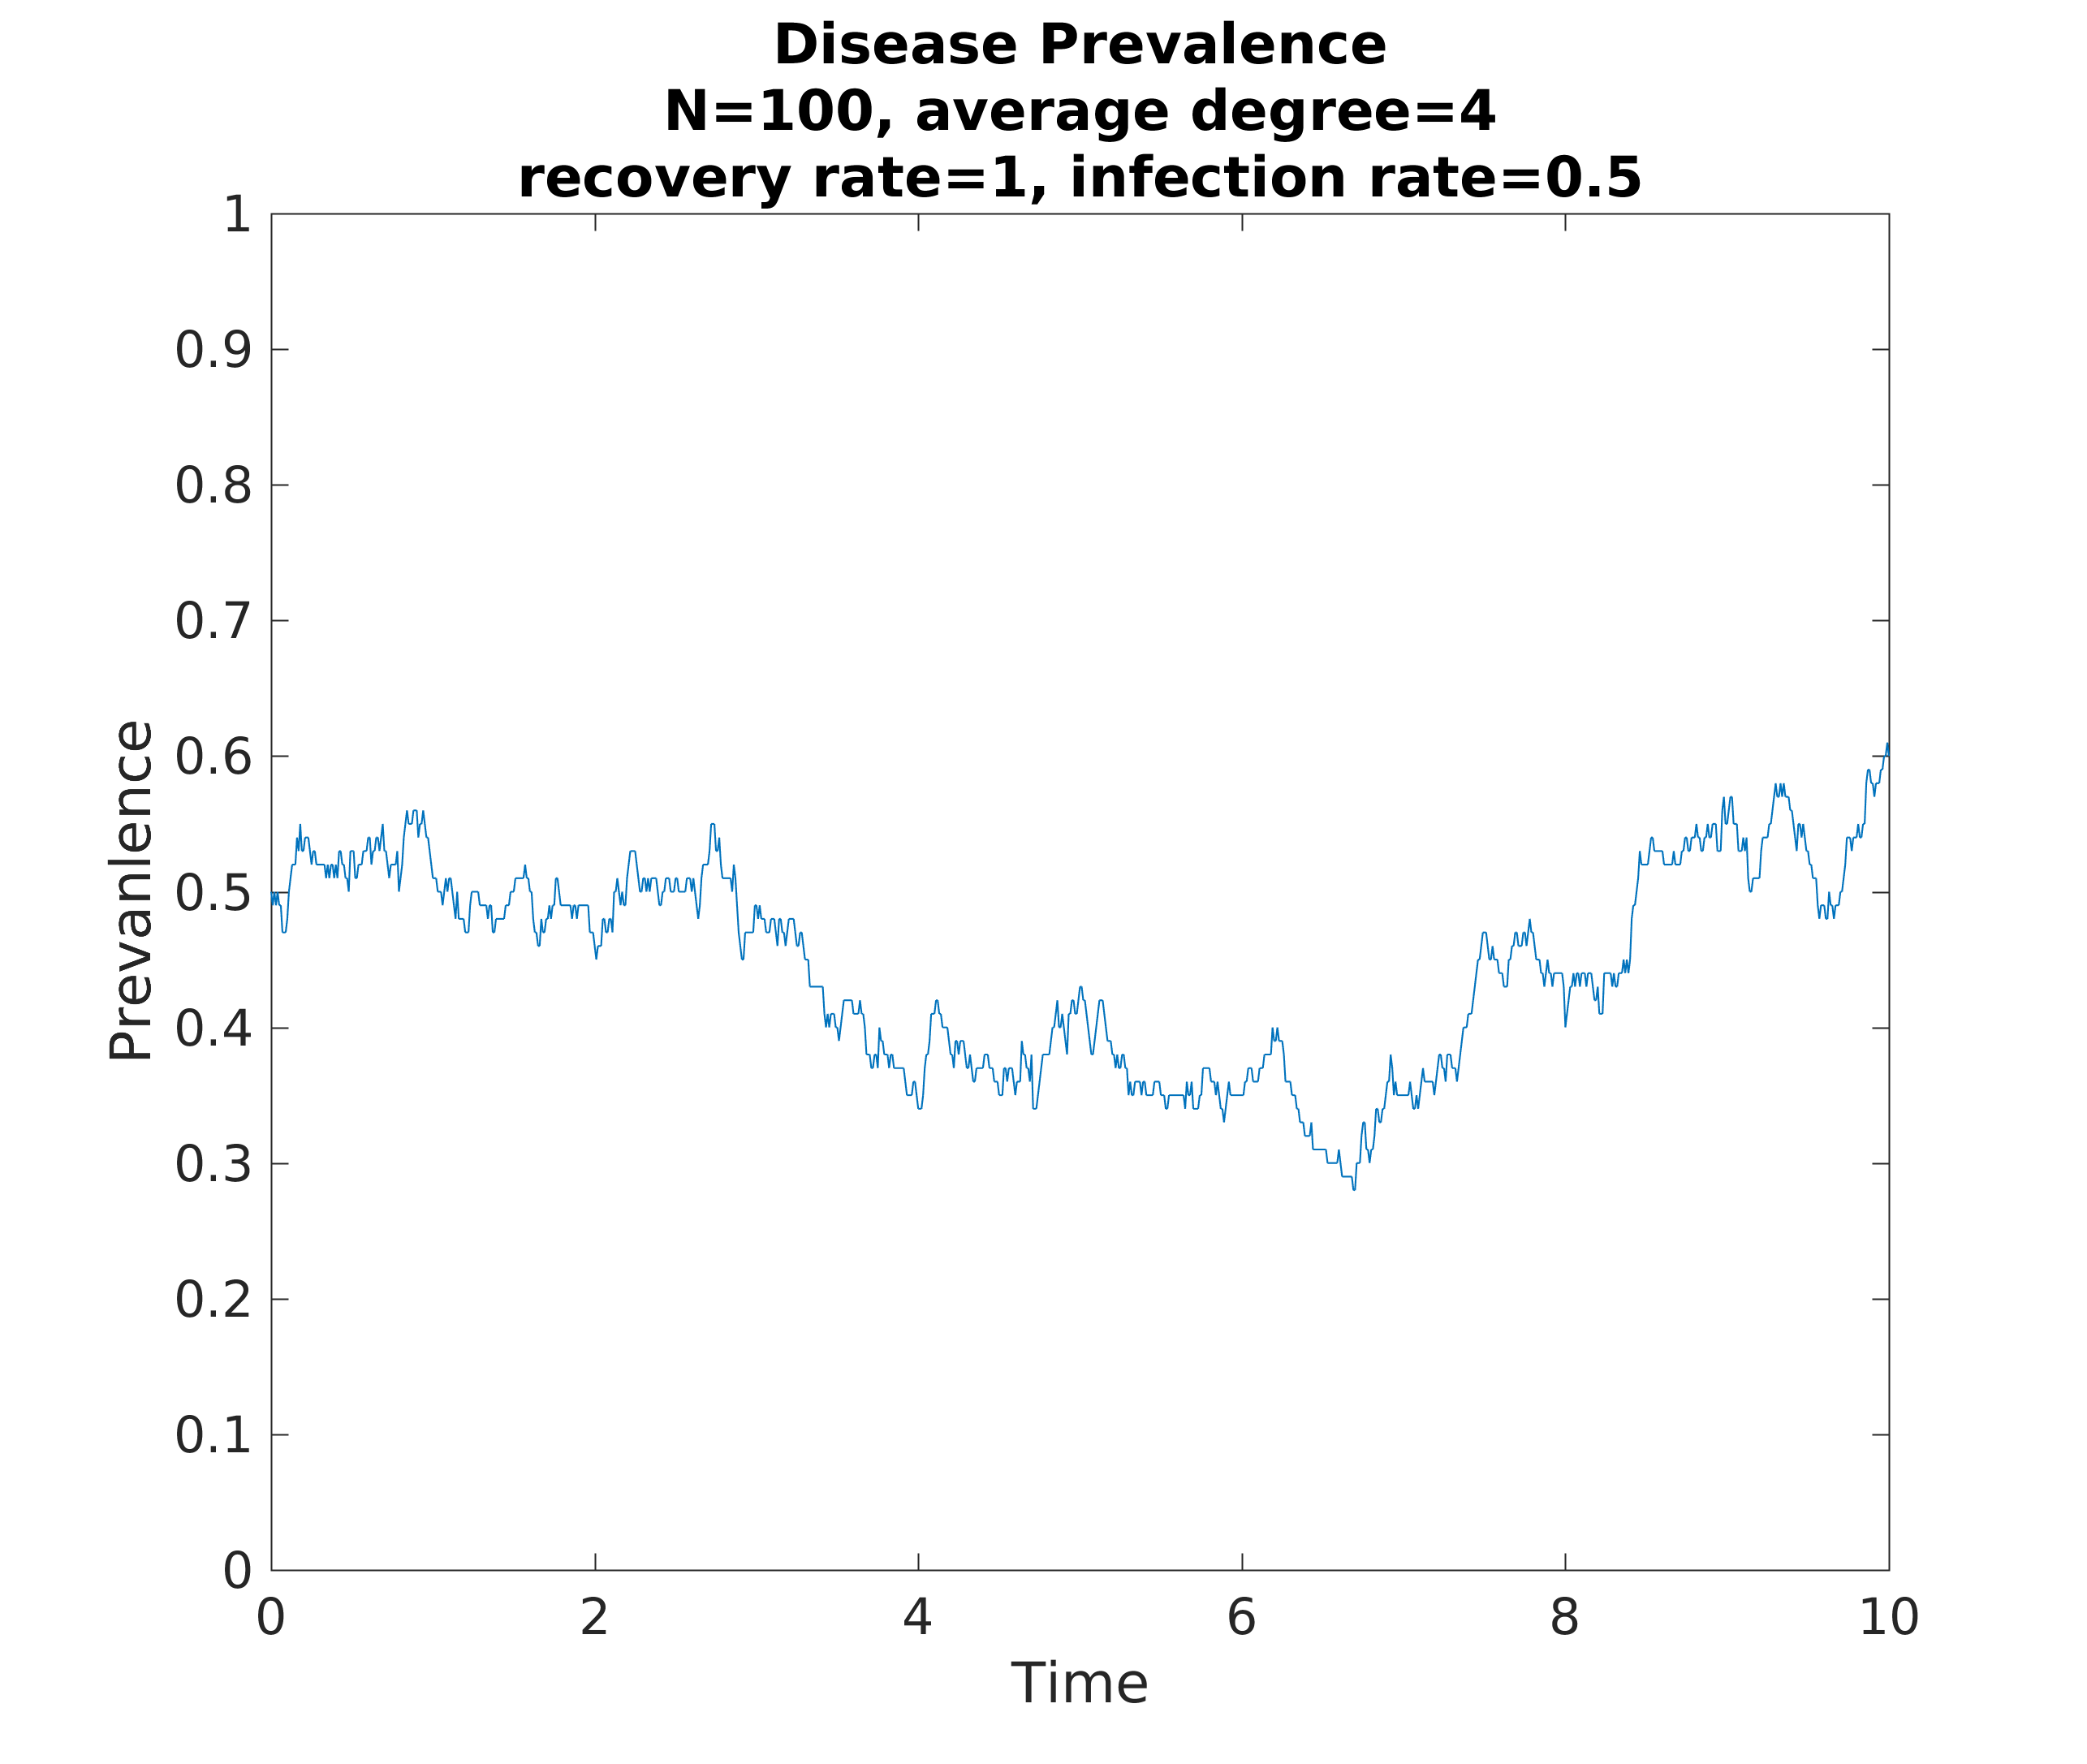
\includegraphics[width=\textwidth]{samplepath10sec.png} 
\end{minipage}
& \begin{tabular}{c}
\\
\\
 $\longleftarrow \,$No rewiring
\\
\\
\\
                                                              \end{tabular}
\\
\begin{minipage}{\linewidth}
\centering
\onslide<2->
\begin{tabular}{c}
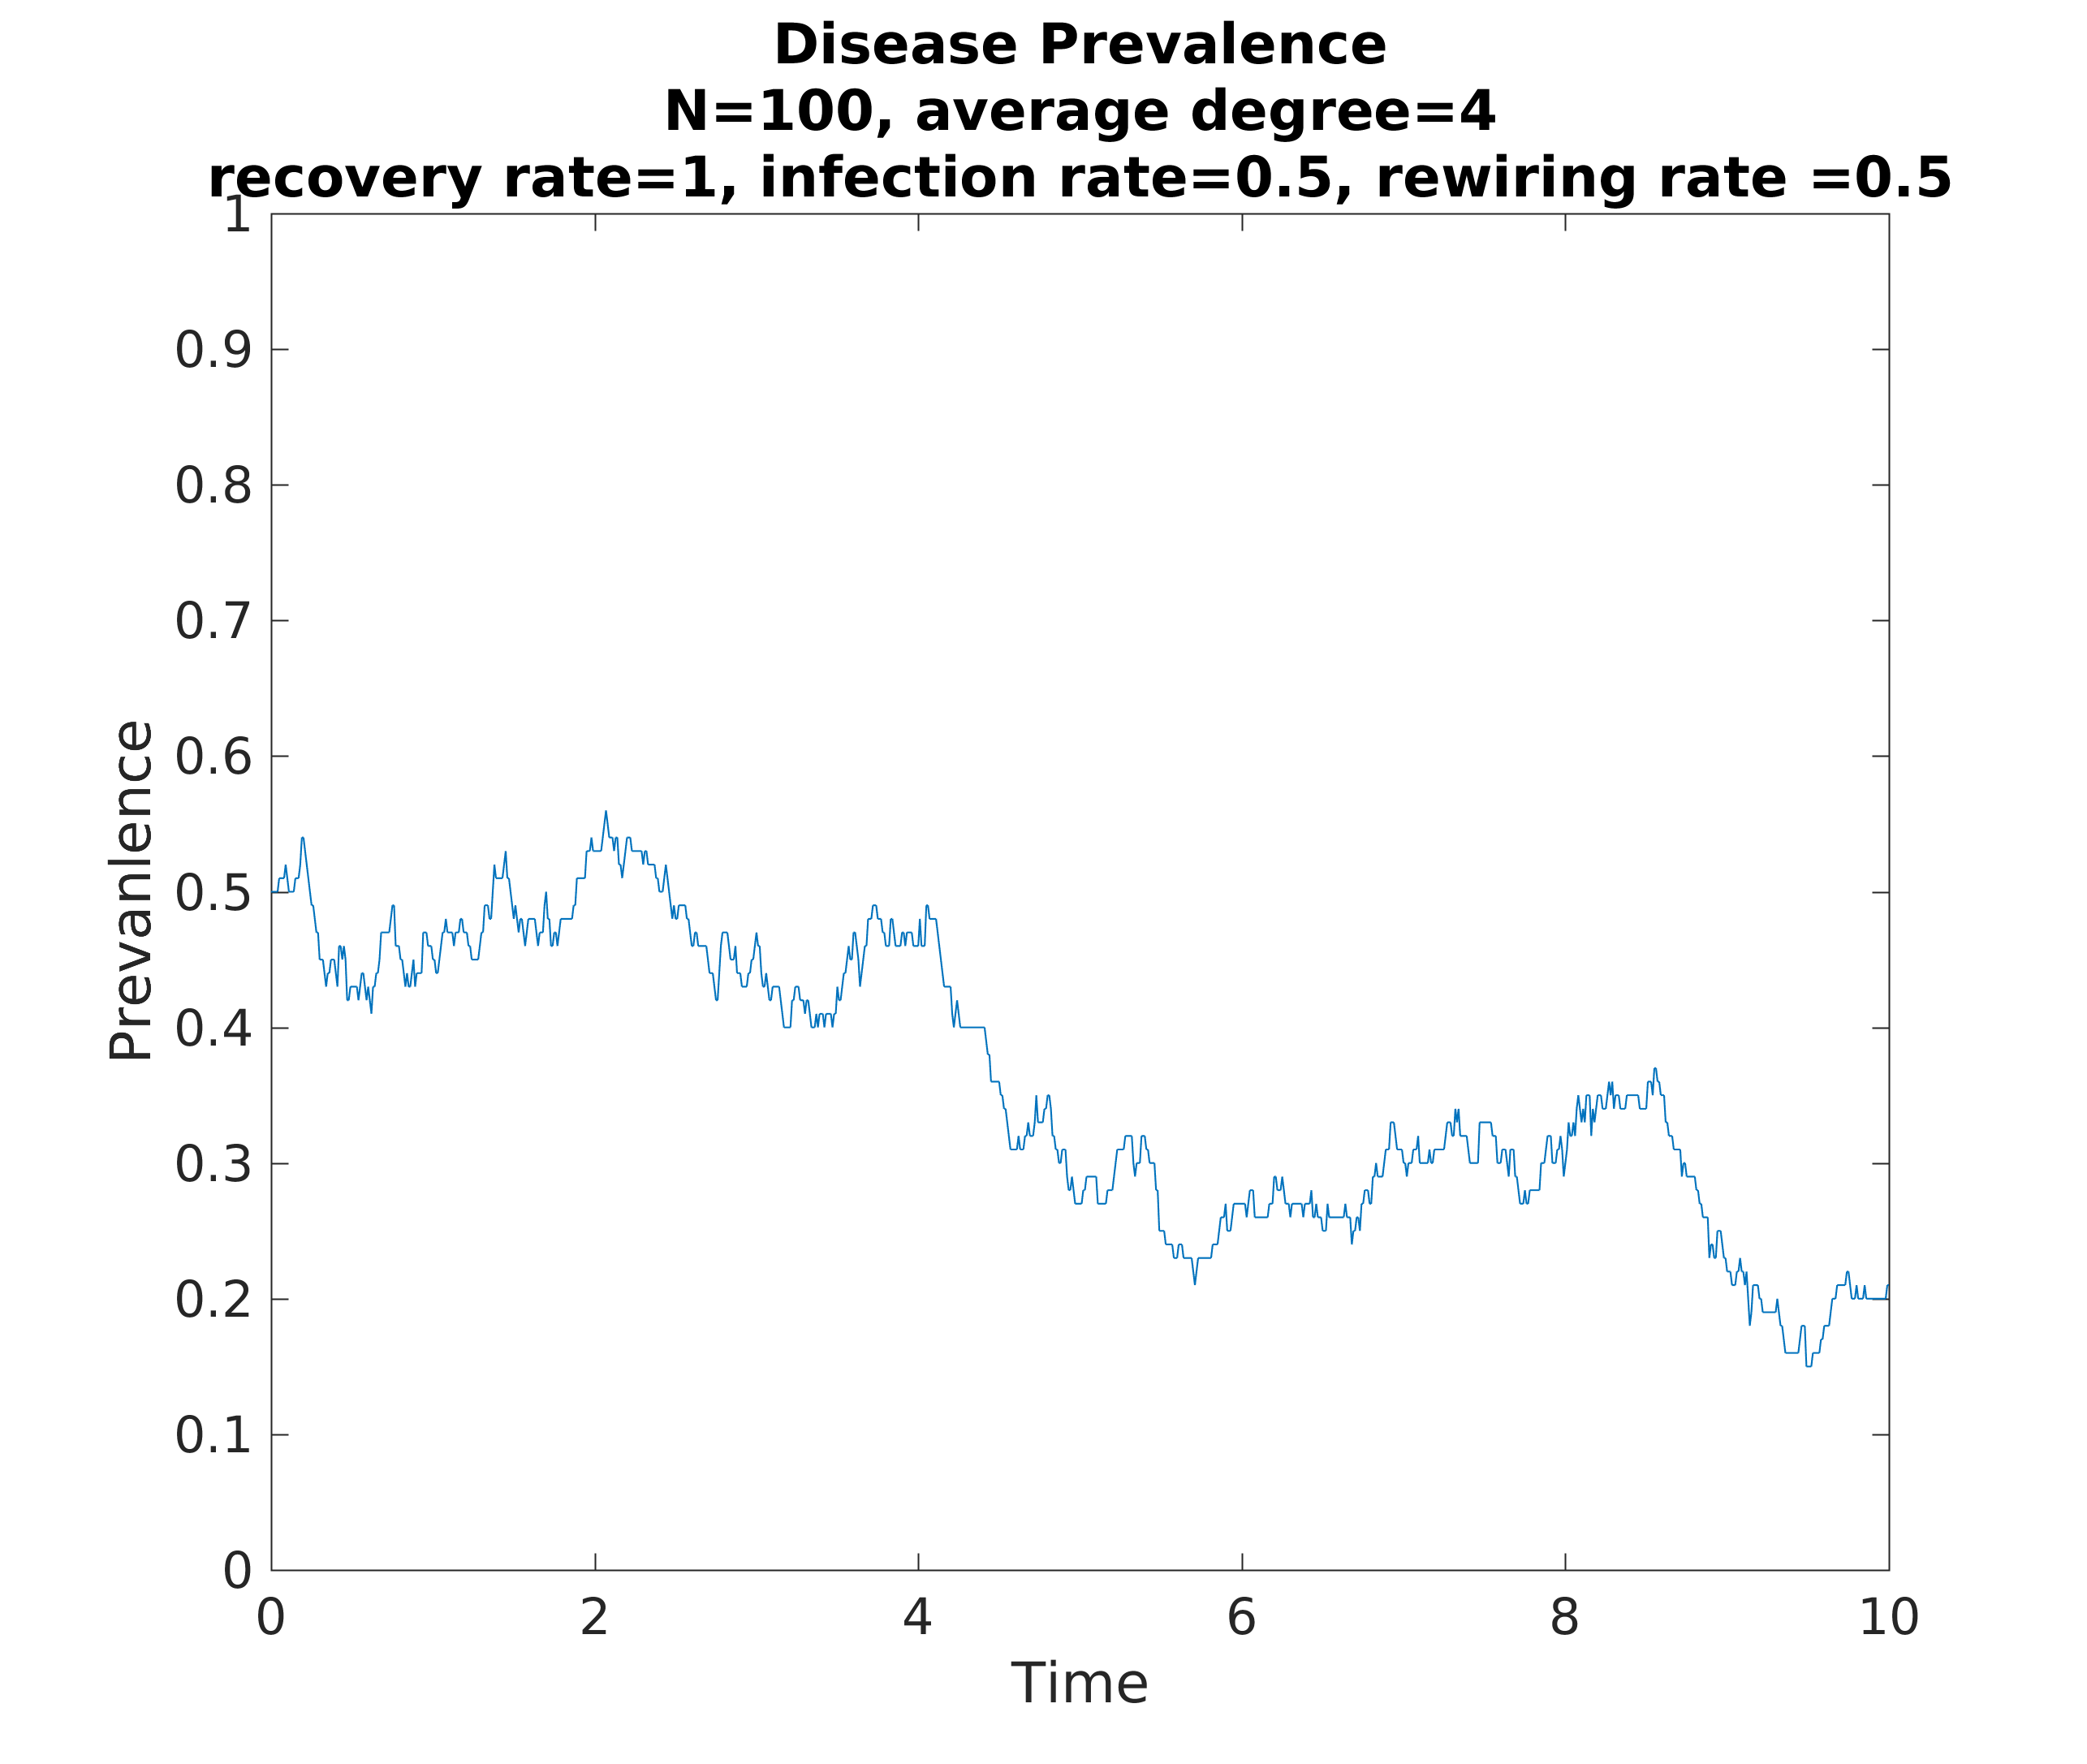
\includegraphics[width=\textwidth]{samplepath10sec05rew.png}\\
rewiring rate $=0.5$.
\end{tabular}
\end{minipage}
&
\begin{minipage}{\linewidth}
\centering
\onslide<3->
\begin{tabular}{c}
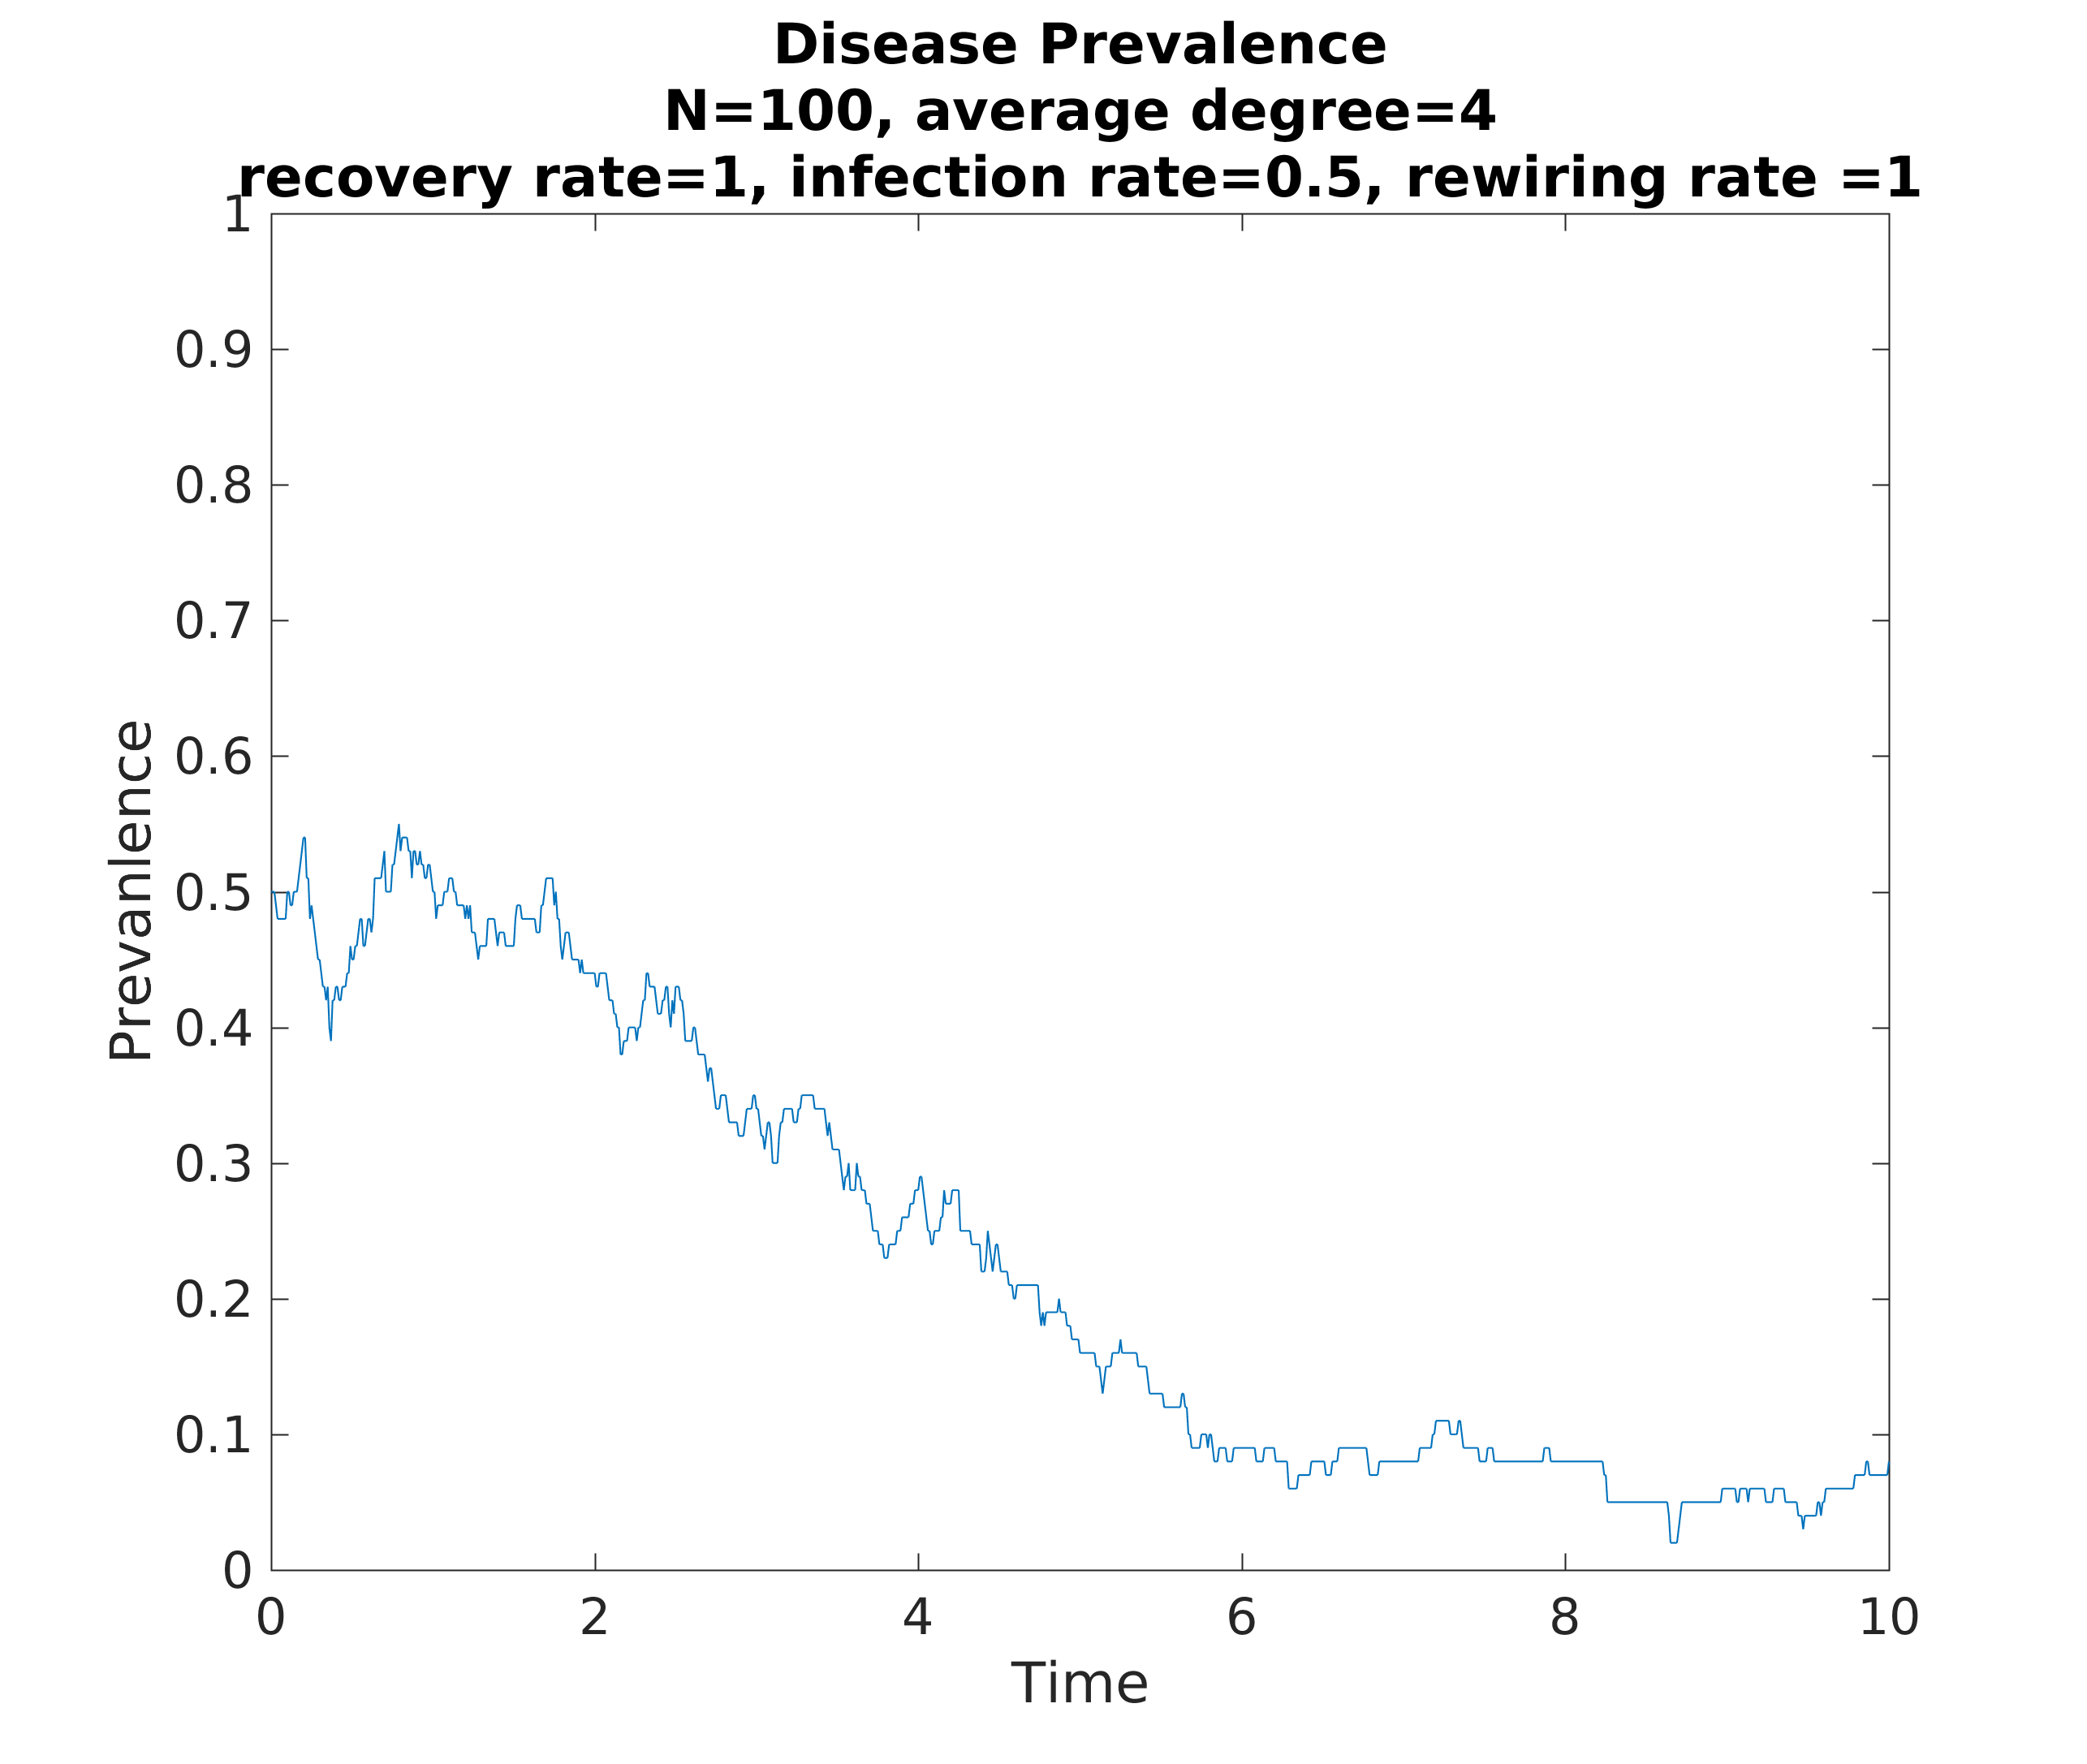
\includegraphics[width=\textwidth]{samplepath10sec1rew.png}\\
rewiring rate $=1$.
\end{tabular}
\end{minipage}
\end{tabular}
}
% \includegraphics[width=.33\textwidth]{samplepath10sec.png}
% \includegraphics[width=.33\textwidth]{samplepath10sec05rew.png}
% \includegraphics[width=.33\textwidth]{samplepath10sec1rew.png}
\end{frame}

\begin{frame}
\frametitle{Thank you}
\centering
Every thing can be found on github.\\
\vspace{3ex}
https://github.com/leomarlo/TalkOnGillespieAlgorithm
\end{frame}


\end{document}
